
\chapter{Introduction}

\section{Connection to Unit 1}
In Unit 1 we reviewed basic concepts of statistics and we introduced
Bayes' Theorem. We  encountered several parameterised probability distributions
and we have seen that if we want to use them to model data processes we
need to be able to estimate parameters from real data. We have seen
that the most widely used method for this is maximum likelihood estimation
MLE. MLE gives a point estimate for the model parameters, which is appropriate
when sufficient data is available. We have also seen that we can adopt a prior
probability distribution over our model parameters, by which we can reflect prior beliefs but also uncertainty
in the model parameters. Bayes' Theorem gives us a way to adapt the prior distribution in the face
of data, and to arrive at a posterior distribution of model parameters, which in general will be more
accurate, but still reflects uncertainty about the model. This uncertainty should be taken into account when
making predictions.

In the notebook examples, we have seen that MLE is prone to overfitting. Bayesian models are
far less subject to overfitting. We have seen that to some extent in the emergence of \emph{regularisation}
when we performed Bayesian linear regression as opposed to ordinary least squares, which is a MLE of
model parameters in linear regression under the assumption of a Gaussian noise model. We have seen that OLE corresponds
to the minimisation of a \emph{loss function}. In Bayesian linear regression, we minimise the same loss function
but a penalty term is introduced that discourages the model parameters from  being large, which is called
a \emph{regularisation} term.

The emergence of regularisation is nice, but does not really explain why Bayesian models are
principally protected from overfitting. Not only are Bayesian models less prone to overfitting, but the evidence
for different models can be compared \emph{a posteriori}. This means that for example a linear or a quadratic fit
can be compared with each other in terms of how well they are supported by the data without the need for
cross validation. This in principle should lead to a more efficient
use of data. Unfortunately, the discussion for the underlying reasons takes up
more space than we have available in the module. A good discussion can be found in sections 3.4
and 3.5 of \cite{bishop2006}. Moreover, a consequent application of Bayesian principles is often very
hard for technical reasons. This sometimes creates a need use to short cuts which then undercut the
advantages of the Bayesian approach.

We will demonstrate this in \emph{logistic regression}. In linear regression, we were able to write
down formulae for the model parameters such that they minimised loss functions. Because we had
analytic expressions for these minima, the loss functions were only an aid in obtaining the desired results and
we had little direct use for them.

In logistic regression we no longer can rely on analytic results because it requires the solution of
non linear equations. Instead we are forced to adopt numerical approximations and find the parameters
that minimise the loss functions by an iterative approach.

Bayesian logistic regression is hard for similar reasons. There is no easy way to find a closed analytic
expression for the posterior distribution. There are three approximation methods, two of which will
be discussed in later units. We will explain the problems  in using Bayesian logistic regression.

Logistic regression can also be seen as the simplest \emph{neural network}. Neural network research
did not emerge from statistical theory or machining at large, but was inspired by ideas about how
the brain might work. For this reason there is still some disparity between statistical and
neural network communities. They sometimes have discovered similar concepts and refer to them by a different
name. We will sketch the development of \emph{Connectionism}, as the discipline of studying neural networks
was called in cognitive science.

\subsection{The Unreasonable Effectiveness of Deep Learning in Artificial Intelligence}
After Unit 1, you might reasonably expect that linear regression is the predominant technique in data science,
since despite its name, it is able to deal with non linear phenomena by the adoption of non linear
functions as basis functions. We have mainly demonstrated regression on univariate models, but in principle
we could for example use two dimensional polynomials as basic functions for two-dimensional
input data, indeed polynomials of any dimension that matches the dimensionality of the input data.
However, modern neural networks deal with
high dimensional data, such as pixels. Even a simple image, like a handwritten numeral has $28 \times 28 = 784$
dimensions. The possible number of polynomials of degree $d$ and number of variables $n$ is given by:

$$
\left(  \begin{array}{c} d+n \\ n \end{array} \right)
$$
To fit a dataset with polynomials of degree 3 in 784 variables, we need to determine the value of 80 million
coefficients! No dataset is rich enough to allow this by linear regression in the way we performed it in Unit 1.

Neural networks in practice have been able to perform reliable classification on images of this size. The reasons
for why this is the case are not fully understood.
The title of this section is taken from a recent paper by one of the pioneers in the field \cite{sejnowski2020}, who
freely admits that he nicked this title from Eugene Wigner's \emph{The Unreasonable Effectiveness of Mathematics in the Natural Sciences}.
It is eminently readable and you should read this on the side.
In this paper some pointers can be found as to why neural networks are efficient. But it mainly emphasises the
inspiration of the brain sciences on their development.

Bishop's view \cite{bishop2006} is that neural networks can be considered as regressors that are able to learn
their own basis functions from the available data and therefore adapt to the particular training set. They do so
with a large number of parameters, but not the astronomical number that would be required for polynomials. Moreover,
modern deep learning uses techniques to keep the number of parameters under control, such as weight sharing. These
methods will be discussed in detail in the \emph{Deep Learning} module.

The large number of parameters involved in the use of multi-layered networks also work against the development
of Bayesian methods. Although Bayesian neural networks have been around for years \cite{bishop1995}, truly Bayesian
neural networks are still in their infancy \cite{jospin2020}. \emph{Variational methods}, which we will discuss
in Unit 5, however have made a considerable impact, in particular \emph{variational autoencoders}.



One of the key results of Connectionism, the branch of cognitive science that uses neural networks,
was the development of an algorithm called \emph{backpropagation by error}.
Although the simple neural networks studied in the eighties of last century have evolved into \emph{deep learning},
it is still useful to study simple examples because the backpropagation algorithm is a mainstay of modern deep
learning and retained its importance for the field. Understanding this algorithm and being able to apply
it in one of the modern neural network frameworks - we have chosen PyTorch - is the most important
learning outcome of this unit.

\subsection{Learning Outcomes}

\chapter{A Brief History of Neural Networks}

The seat of soul has been placed in various parts of the body throughout history. It is only at the end of the 19th century
that a clear hypothesis about the brain as an information processing unit start to emerge. Important influences were
von Helmholtz's measurements of nerve speed, which helps to establish nerve function as an electrical phenomenon and
the emergence of Golgi staining, which made it possible to study neurons for the first time. Without staining brain tissue
is transparent under the microscope leading to a wide variety of theories about its possible constituents. A Spanish neuroscientist,
Ramon-y-Cajal used this staining method to great effect to make beautiful and intricate pictures of groups nerve cells (Fig. \ref{fig-draw}).

\begin{figure}[!ht]
  \begin{center}
    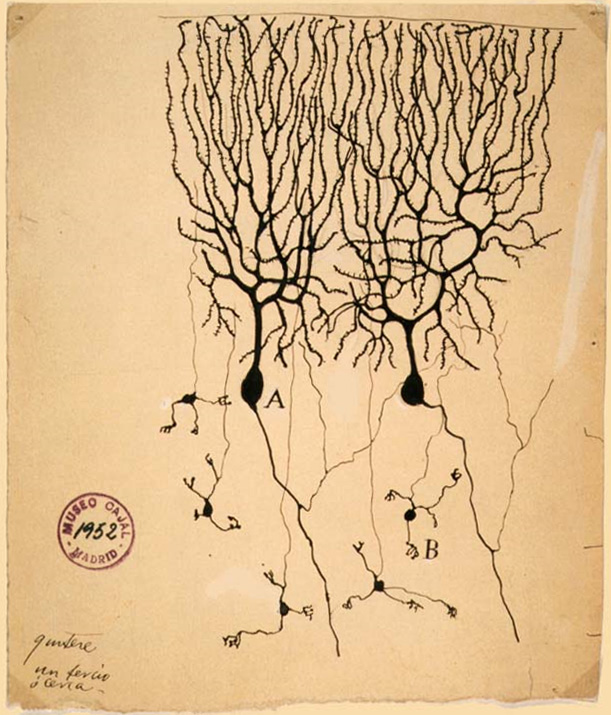
\includegraphics[width=0.7\textwidth]{PurkinjeCell.jpg}
  \end{center}
  \caption{Drawing of a Purkinje cell (a type of neuron by Ramon-y-Cajal.}
  \label{fig-draw}
\end{figure}

His and others' observations led to the \emph{neural doctrine}, which among others states that \url{https://en.wikipedia.org/wiki/Neuron_doctrine}:
\begin{itemize}
\item The brain is made up of individual units that contain specialised features such as dendrites, a cell body, and an axon.

\item These individual units are cells as understood from other tissues in the body.

\item Although the axon can conduct in both directions, in tissue there is a preferred direction for transmission from cell to cell.

\end{itemize}

\begin{figure}[!ht]
  \begin{center}
    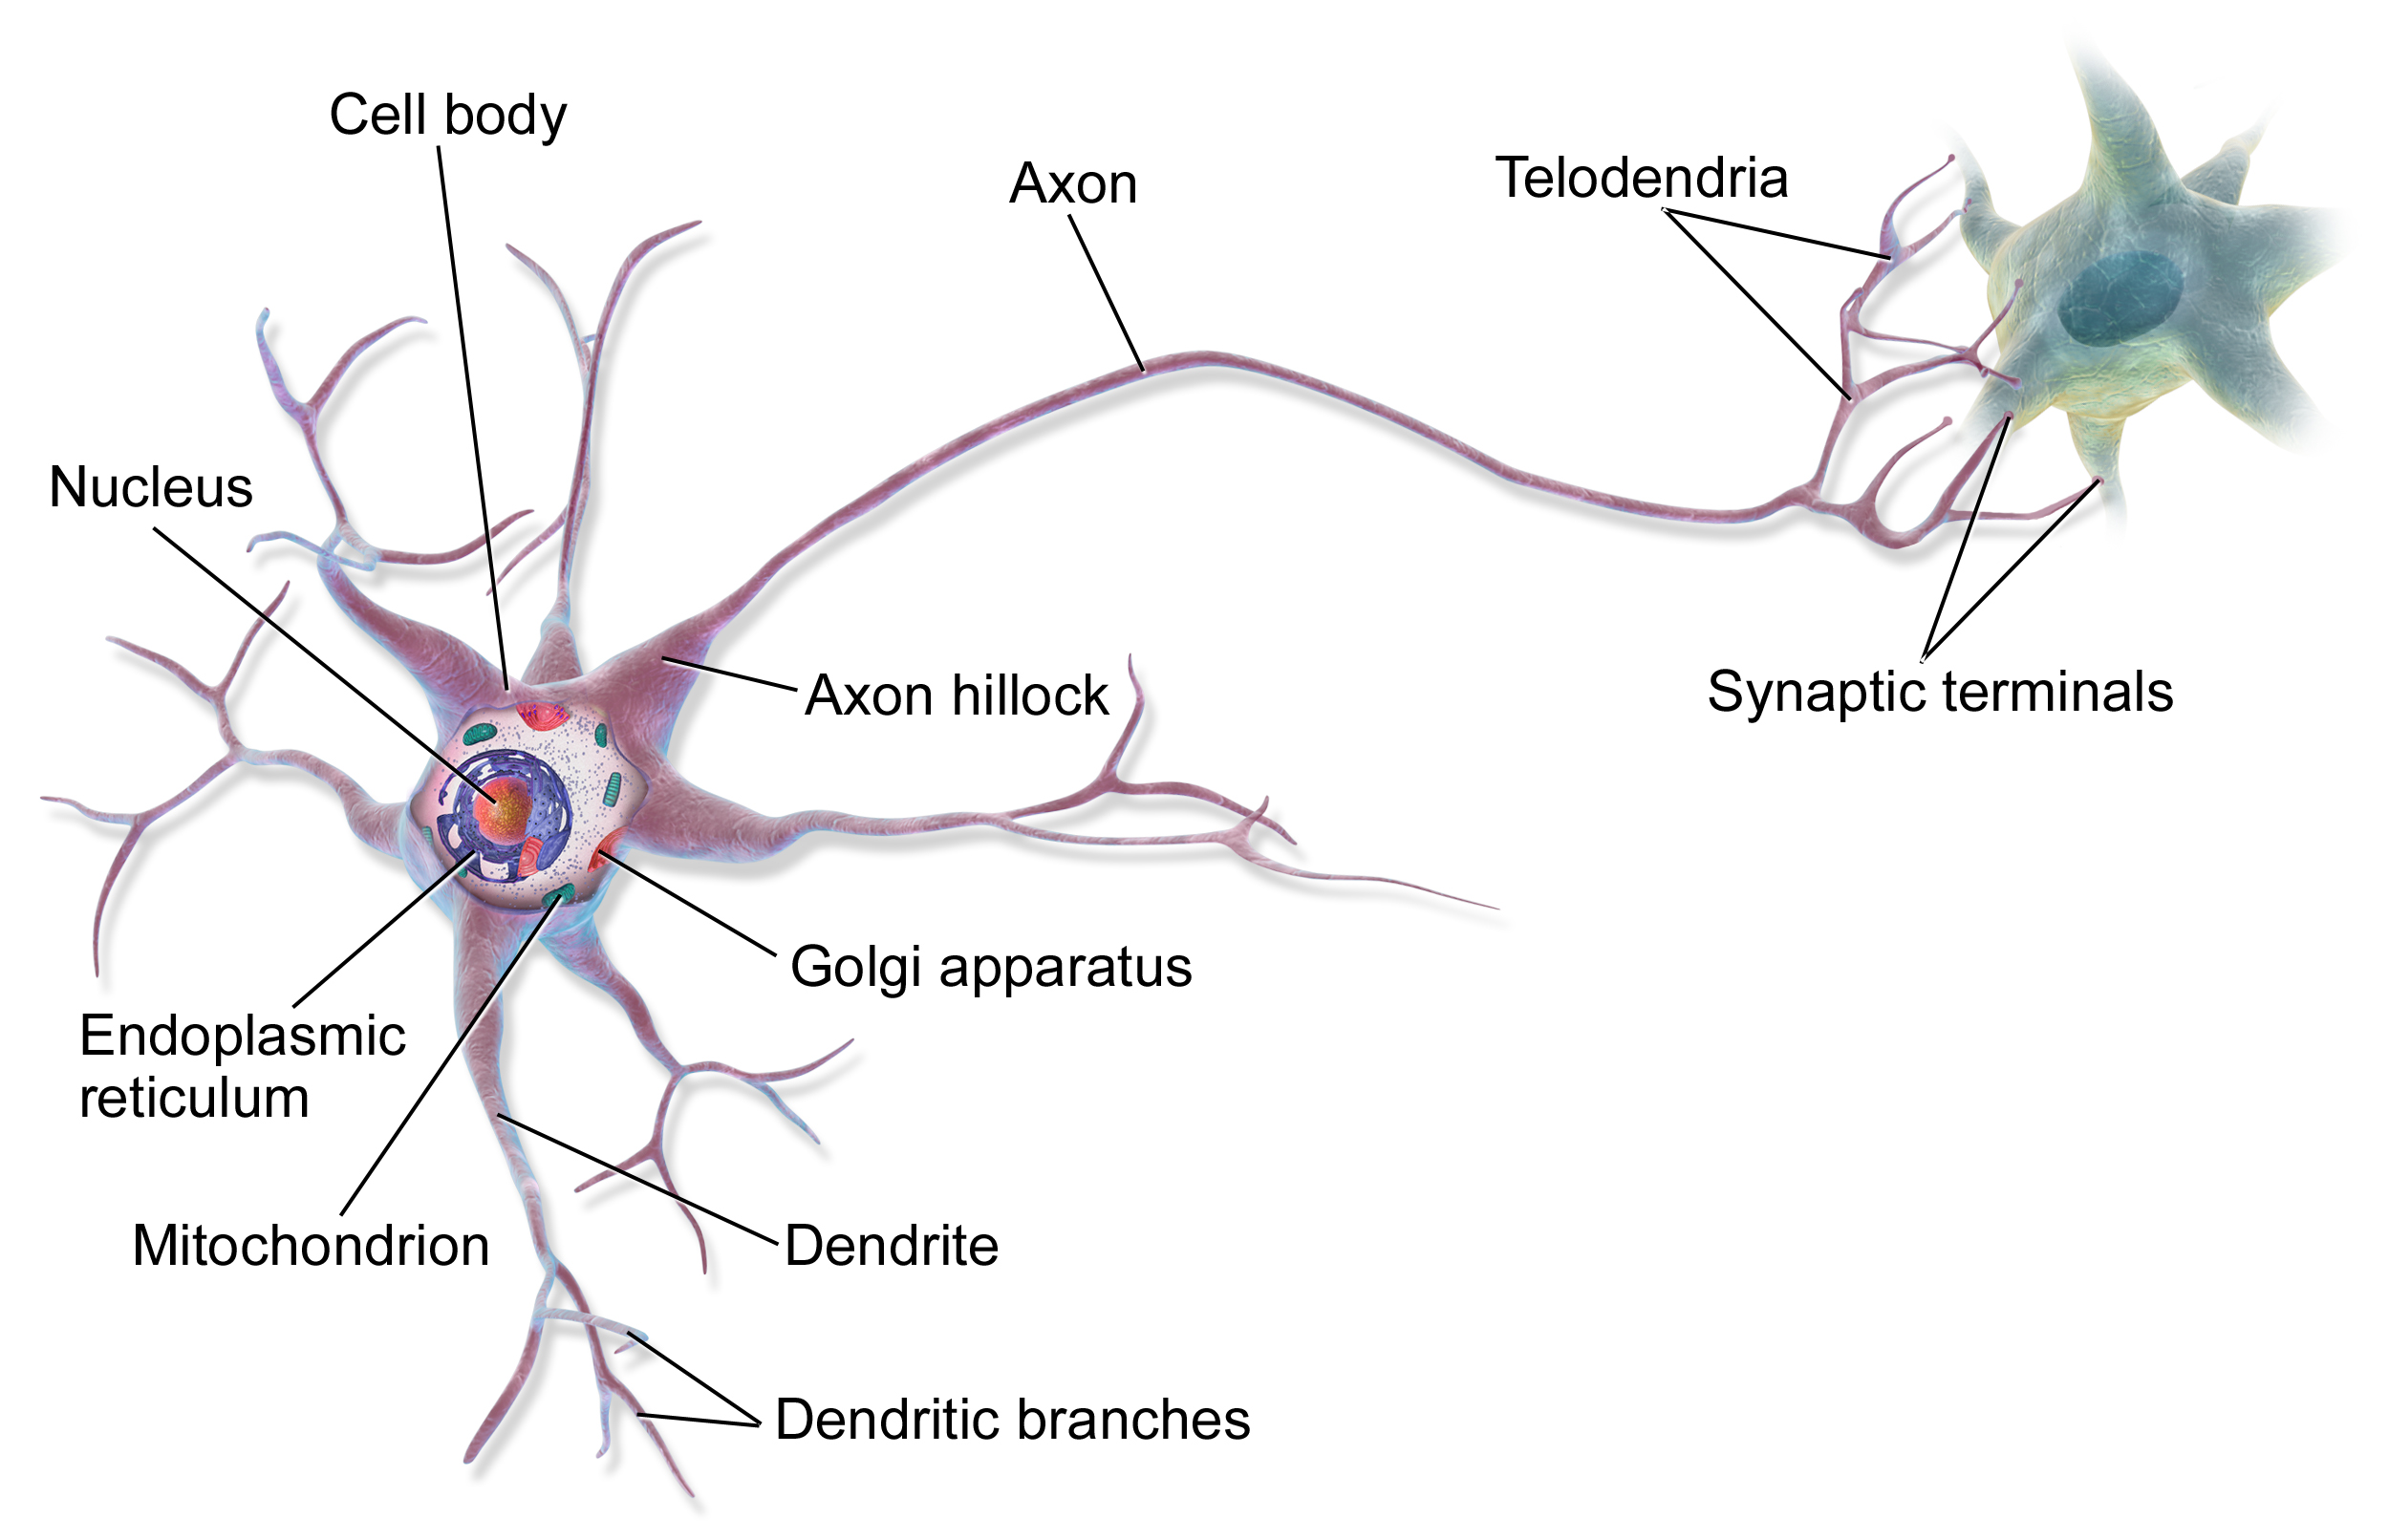
\includegraphics[width=0.7\textwidth]{Blausen_0657_MultipolarNeuron.png}
   \end{center}
  \caption{A schematic representation of a biological neuron.}
  \label{fig-biological}
\end{figure}

The neuron doctrine is an important step forwards because it recognises neurons as the most important functional part of the brain, that neurons are
cells, and that there is a clearly defined flow of information. Further experimental progress was made by many experimentalists, notably by
Hodgkin and Huxley, who deducted the  ion pump mechanisms that allow the neuron to be an electrochemical cell from electrophysiological
measurements, later confirmed experimentally. By that time, the idea
of the neuron as an information processing unit had taken hold. McCullogh and Pitts (1943) demonstrated that complex Boolean functions
can be implemented by networks of artificial neurons, which are an important precursor to the artificial neurons that are used today.

There are many mechanisms by which neurons communicate with each other, but a predominant one is the following:
neurons have a dendritic tree. Other neurons connect to the dendritic tree via \emph{synapses}. They can release so-called
\emph{neurotransmitters}, which can alter the properties of ion channels of the receiving neurons. The effects can be \emph{excitatory}
or \emph{inhibitory}. Ordinarily, a neuron maintains a negative potential difference between the inside and outside of the cell membrane.
Upon the reception of an excitatory event neurons locally \emph{depolarise}, i.e. become a little bit less negative. If nothing else
happens, this \emph{equilibrium potential} is restored within approximately 10 ms. If several such events heap up, the neuron depolarises so much that
a spontaneous chain of depolarisation takes place, that will travel along the cell body and then further along the cable-like \emph{axon}. This process
resembles a fuse more than electric pulse conduction.
This potential change is rapid and large, and for that reason is called a \emph{spike}. It spreads spatially.  This spike, when it has travelled down the axon causes the
opening of so-called synaptic vesicles, which contain neurotransmitter. They can travel through the fluid surrounding the neurons and transverse
the synaptic cleft to influence other neurons in turn.

If neurons receive only a small number of excitatory events, the depolarisation returns to equilibrium. Inhibitory events prevent depolarisation
from building up. Only if a sufficient number of spikes arrive at the dendritic tree the local depolarisations can be so strong that a spike event will
be caused. To some extent, one can think of this as a threshold. Unless depolarisations build up to a so-called threshold potential, neurons do not
communicate with other neurons. Only spike events are communicated between neurons, not the sub-threshold dynamics leading up to them.
This is a highly simplified picture for sure: in the famous Hodgkin-Huxley \cite{hodgkin1952} model, a system of differential equations that describes the
ion movements across the neuron membrane and the resulting potential differences, you will not find a threshold, but the picture is
useful and has stuck:

\emph{Key idea: A neuron integrates its input, and only responds if the net input crosses a certain threshold.}

So, real neurons are a complex electrochemical system. In the Petri dish, we understand this system reasonably well. There is a whole area
of science dedicated to predicting the behaviour of individual neurons in response to electrical and chemical manipulations: \emph{computational
  neuroscience}. If the brain is a massive pile of neurons, some of which are stimulated by sensory input, driving other neurons, most only communicating
with other neurons and some driving muscles, thereby implementing actuations, then where are our thoughts, feelings and memories? Somehow, they must be
carried by the distributed activities of the neurons. And in this highly dynamic environment, how do we consolidate memories over our entire lifetime?
The last question has an answer to some extent. It is agreed that an important component driving memory formation is formed by changes in the
efficacy by which neurons influence each other. Such changes can be driven by the activation of the neurons themselves, so-called spike time
dependent plasticity. An important example of this is the observation that neurons that are connected and fire within a given time window in the future
are more likely to fire together if one of them receives stimulation, a principle that is called 'fire together - wire together'. It is the dominant view
of the neurosciences as well as cognitive science that responses of the nervous system to outside stimuli are ultimately implemented in the form of
synaptic efficacies. The learning of new behaviour and the formation of new memories entails changing these efficacies. There is substantial
experimental evidence that behavioural changes indeed are associated changing synaptic efficacies, or the formation of new synapses, or the development
of white matter tracts, which are an insulating sheet around the axons, and therefore indicate the formation of new connections. A recent paper
\cite{abraham2019} contains references to material supporting this view, but also points out that this general idea is very hard to proof conclusively, and that
other mechanisms than synaptic plasticity may also underlie \emph{learning}.

Nonetheless, the field of artificial neural networks has absorbed this idea:

\emph{Key idea: learning in an artificial neural networks is enacted by changing the efficacy by which neurons can influence each other.}

In artificial neural networks synaptic efficacies are represented by real numbers and we will see examples of how artificial neural networks
and their connections are represented in the sections below.


\chapter{Perceptron and Linear Discriminants}
\subsection{The Perceptron}

\begin{figure}[!ht]
  \begin{center}
    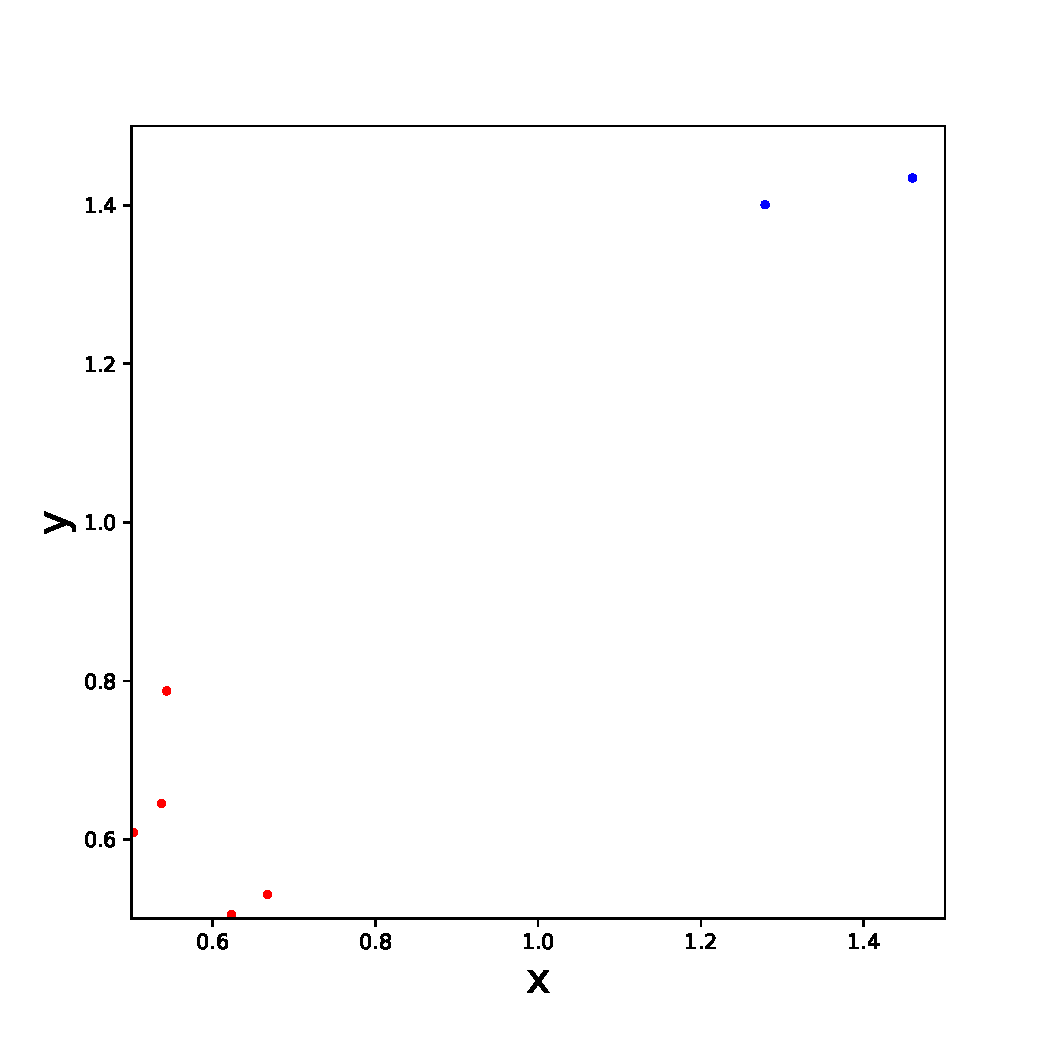
\includegraphics[width=0.7\textwidth]{linsep.pdf}
  \end{center}
  \caption{A dataset, consisting of measurement values which have been classified as belonging two one of two classes.}
  \label{fig-linsep}
  \end{figure}
    
A key idea in the development of neural networks is  Rosenblatt's perceptron. It is no longer used as a serous machine learning technique, but it is an excellent
device to demonstrate some of the key principles that underpin neural networks. Consider Fig. \ref{fig-linsep}. Here, two quantities $x$ and $y$ have been measured,
and the measurement values have been \emph{classified}. For example, $x$ and $y$ are two chemical concentrations, and the classification can be hazardous
or non-hazardous. Based on the data sample that has been classified thus far, it seems that the two classes are well separated in terms of concentration space $(x,y)$.
If future measurements behave similar, it will not be difficult to design a \emph{classifier}. One way of doing that is to draw a straight line between the two sets of points,
and if a new data point arrives it can be classified according to which side of the line it falls. This is the idea behind a \emph{linear classifier} (or discriminant).

Mathematically, we can implement this by representing the line between the two classes, the so-called \emph{decision boundary} in terms of its parameters. The most general
representation of a straight line in two dimensions is:
$$
ax + by = c
$$
and we can implement a decision by using a so-called \emph{squashing} function, which here we take to be the Heaviside or step function:
\begin{equation}
  o = \mathcal{H}(ax + by -c),
  \label{eq-decision}
\end{equation}
with
$$
\mathcal{H}(x) = \left\{ \begin{array}{cc} 0 :  x &  < 0 \\ 1: x & \ge 0 \end{array} \right.
$$

Note that we need all three parameters: without $c$, we would only be able to represent lines through the origin, which would not do for the dataset of Fig. \ref{fig-linsep}.
The more commonly used representation of a straight line $y = ax + b$ is unsuitable because vertical lines can not be represented, and near vertical lines would
require large parameters, something which is generally undesirable, consider for example, the discussion on regularisation in Unit 1.

Inspired by neuroscience, we can introduce an artificial neuron with two inputs, and a weight associated with each input. In general, we write:
\begin{equation}
  o = f(w_1 x_1 + w_2 x_2 -\theta)
  \label{eq-perc}
\end{equation}
This is nothing but a rewrite of Eq. \ref{eq-decision} of course. Our parameters $w_1, w_2$ are now called weights, and $\theta$ is called a \emph{threshold} or
\emph{bias} (we will treat these words as synonyms).
$x_1$ and $x_2$ are just our former variable $x$ and $y$.

The device represented by Eq. \ref{eq-perc} is called an \emph{artificial neuron}. Calculating the \emph{output state}, the value of variable $o$ is called \emph{updating}
the neuron (we often drop the adjective artificial is this is clear from the context). Often, the output state is retained until a new update is made, for example in
response to changed inputs.

Note that conceptually there are similarities to the real neuron: one could consider the quantity $w_1 x_1 + w_2x_2$, the so-called \emph{local field} as a representation
of the fact that the weighted input contributions exceed the threshold $\theta$, or not. If the threshold is not crossed, the response will be '0'. Like the real neuron, the
artificial one is not affected by sub threshold activities, but if the threshold is exceeded, a non linear response follows: a sudden jump to '1'.  Later, it will turn out that these non linearities are very important.




To illustrate both the process and also provide an illustration of McCullogh and Pitts point that networks of artificial neurons can implement complex Boolean functions, let
us look at the logical {\bf AND} gate as a classification problem.

\begin{table}[!ht]
  \begin{center}
  \begin{tabular}{||c|c||c||} \hline \hline
    $x_1$ & $x_2$ & $o$ \\ \hline
    0   &  0  & 0 \\
    0   &  1  & 0 \\
    1   &  0  & 0 \\
    1   &  1  & 1 \\ \hline
  \end{tabular}
  \end{center}
  \caption{The {\bf AND} gate as a classification problem. It can be considered such because $x_1$, $x_2$ can be considered its inputs and the required
    logical value is the desired output classification.}
  \label{tab-and}
\end{table}


The 4 input values can be represented as  points in $x_1, x_2$ space and can be plotted with a marker to indicate whether the desired classification is '0' or '1'.
The resulting figure, Fig. \ref{fig-and}, is similar to  Fig. \ref{fig-linsep} in that it is clear that a straight line can be found that separates the class '1' point
from the class '0' points.

The equation of the line in the figure can easily be seen to be
$$
y = -x + 1.5
$$
We only have to do a simple rearrangement to bring this into perceptron form:
$$
x + y - 1.5 = 0
$$

\begin{figure}[!ht]
  \begin{center}
    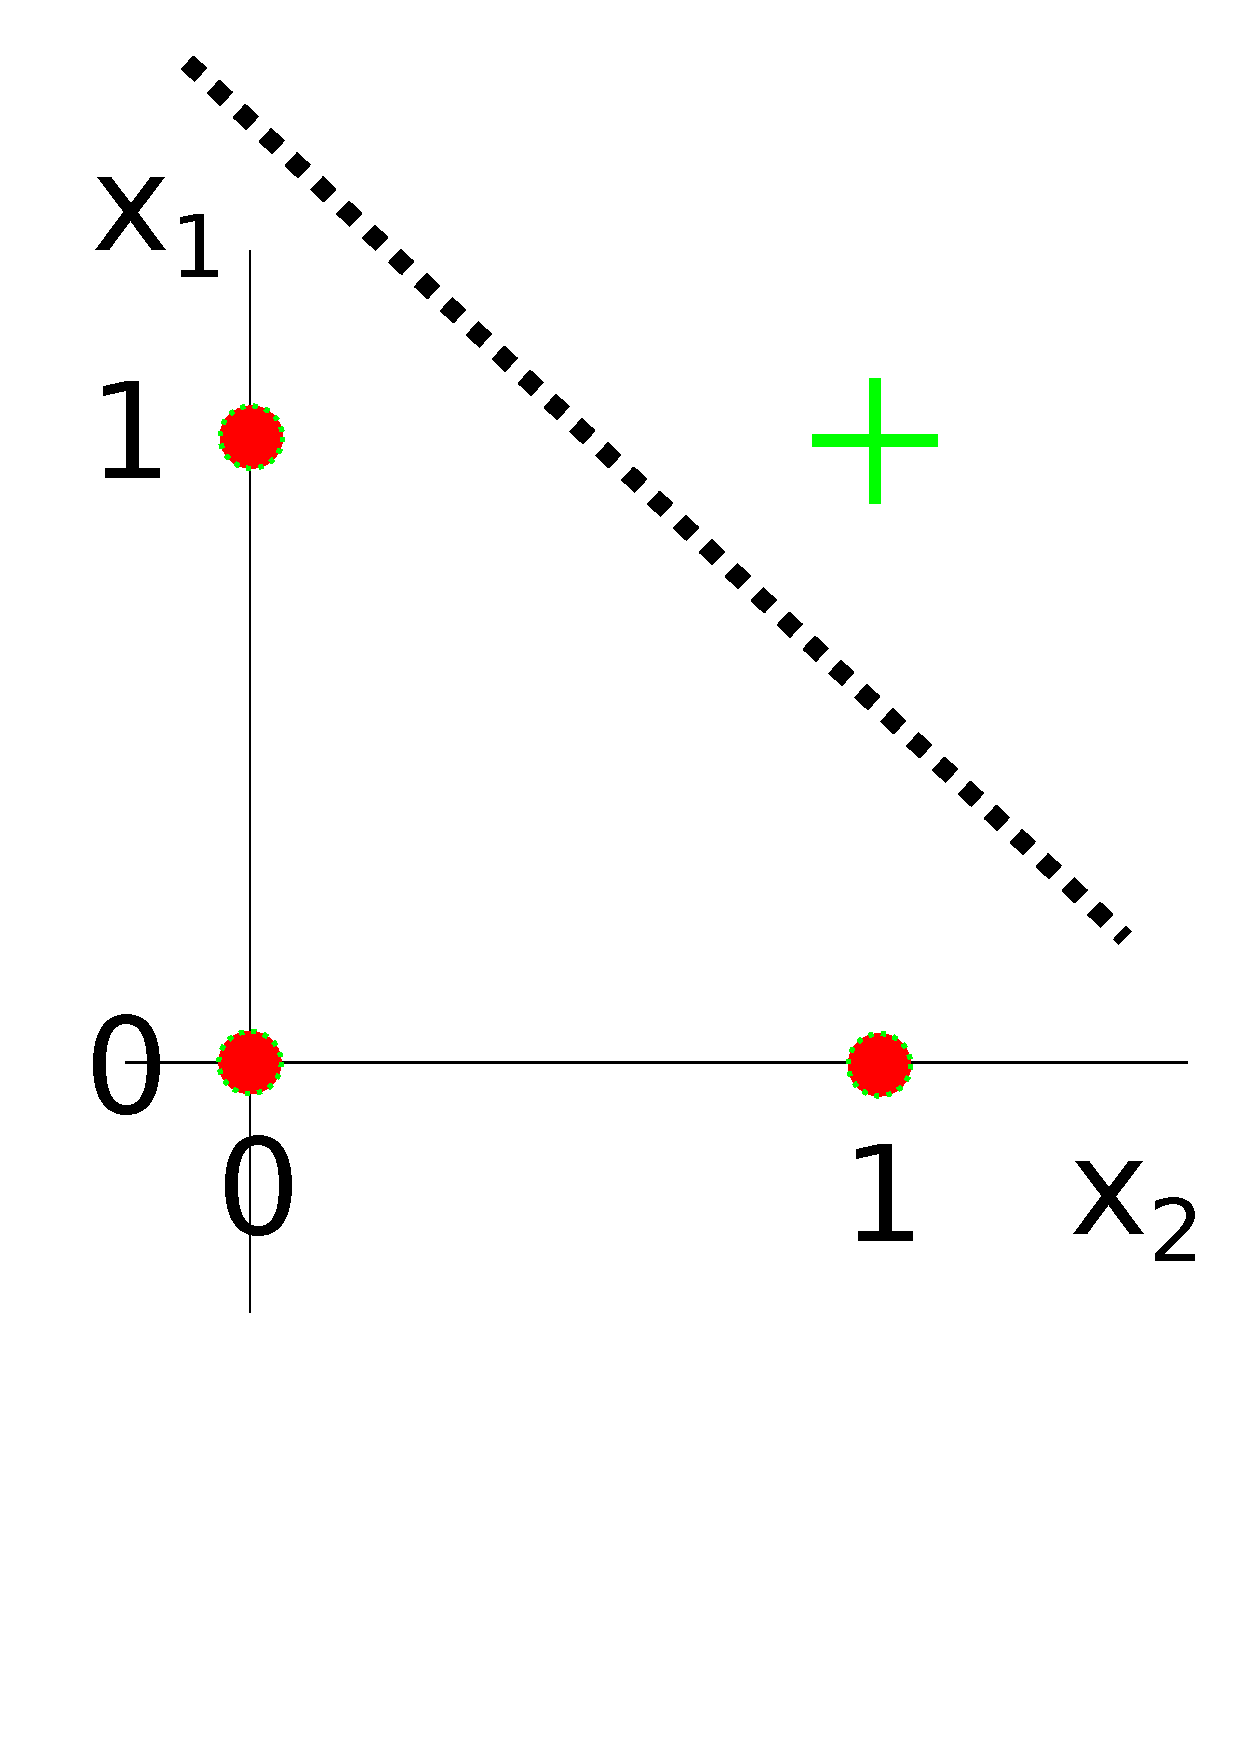
\includegraphics[width=0.7\textwidth]{and.pdf}
  \end{center}
  \caption{The AND gate as a classification problem is linearly separable.}
 \label{fig-and}
\end{figure}



We now have to decide which points should have outcome '0', and we chose:
\begin{equation}
  o = \mathcal{H}(x_1 + x_2 - 1.5)
  \label{eq-percthresh}
\end{equation}
From this, we can read off weights and threshold: $w_1 = w_2 =1$, $\theta = 1.5$. Note that the value of the threshold itself is a positive value, the minus sign in
Eq. \ref{eq-perc} ensures it works as a threshold.

So far, we have only determined the position of the decision line, but the decision could go the wrong way and we need to check that we have not accidentally chosen
the inverse classification!
We try the point $(0,0)$. This gives:
$$
1 \cdot 0 + 1 \cdot 0 = 0 < 1.5
$$
The weighted sum is less than the threshold, so the output classification is '0', as it should be. The fact that the other points to be classified as '0'
are on the same side the line and the one that is to be classified as '1' ensures that our classifier is correct. Repeating the calculation for the other values
in the table we see that the only input able to overcome the threshold is: $x_1 = x_2 =1$. This shows why the classifier works.


Now consider the following questions:
\begin{enumerate}
\item Does multiplying all weights and threshold by the same constant change anything in the classifiers output?
\item Does it matter whether this constant is positive or negative?
\end{enumerate}

From the figure it is clear that our perceptron has a nice property: it is fairly \emph{robust}. If the input values are slightly distorted due to noise, the classification
works correct, at least for this line.

It is also clear that the threshold plays an essential role: without it, we would only be able to form decision lines through the origin, and the {\bf AND} problem can not
be solved that way. Later, when we start to develop algorithms to adapt weights to the classification problem at hand, it will become inconvenient to distinguish
between weights and threshold. Like the weights, the threshold may have to be adapted and it will be awkward to have to treat the weights and threshold separately.


A simple solution consists in creating a third input whose input is always equal to 1. The weight of the third input $w_3$ can then be chosen to be
$-\theta$. This means that we have to create a three input perceptron \emph{without threshold} that is capable of learning the following dataset.


\begin{table}[!ht]
  \begin{center}
  \begin{tabular}{||c|c|c||c||} \hline \hline
    $x_1$ & $x_2$ & $x_3$ &$o$ \\ \hline
    0     &  0    &  1    & 0  \\
    0     &  1    &  1    & 0  \\
    1     &  0    &  1    & 0  \\
    1     &  1    &  1    & 1  \\ \hline
  \end{tabular}
  \end{center}
  \caption{The dataset of the {\bf AND} classification problem for a perceptron with three inputs without threshold.}
  \label{tab-andthreshold}
\end{table}

It is clear that the perceptron that is defined by:
$$
o = \mathcal{H}( w_1 x_1 + w_2 x_2 + w_3 x_3)
$$
for $w_1 = w_2 = 1, w_3 = -1.5$ classifies all points correctly and essentially performs the same computation as the perceptron from Eq \ref{eq-percthresh}.

This trick also works in higher dimensions. In general, for any arbitrary hyperplane in an $N$-dimensional space, we can find a corresponding one
that goes through the origin of an $N+1$ dimensional space. 


This is highly convenient, because computationally the calculation of a perceptron output requires the evaluation of the scalar product:
$$
\boldsymbol{w}^T\boldsymbol{x}
$$
Remember from Unit 1 that this is a condensed way of writing:
$$
\sum^N_{i=1} w_i x_i
$$

So, to summarise: we need a threshold or bias to obtain a working classifier but can easily implement this by concatenating the input vector with an extra unit whose
value is always one, and therefore do not need to consider thresholds as anything else but an extra weight in actual calculations.

\section{The Perceptron Algorithm}
It is clear that if a dataset is linearly separable that a perceptron can be found to classify it correctly. This is true in higher dimensional spaces as well.
In $N$ dimensions, we need $N$ weights and one threshold $\theta$. So, we can use a perceptron with $N$ inputs to implement any plane
$$
w_1 x_1 + w_2 x_2 + \cdots w_N x_N = \theta
$$
as a decision boundary, or alternatively, we can use a perceptron with $N+1$ inputs as long as we guarantee that one of the inputs is clamped to the value 1.

If a hyperplane can be found that separates data points into two classes, again, we call this dataset linearly separable and  by definition, a perceptron
can be found that will classify a linearly separable dataset correctly. In higher dimensional spaces the dataset becomes more difficult to visualise, so the graphical
method that we used to determine the decision boundary for the {\bf AND} problem is no longer suitable. Ideally, we would want an algorithm that is capable of
automatically finding the weights given the dataset. For linearly separable datasets a simple algorithm exists that  iterates through the dataset
and finds a correct set of weights in a finite number of steps.

The algorithm is of great historical significance and bears an interesting relationship to \emph{logistic regression}, which we will discuss later in this Unit. Nowadays,
it is longer the method of choice due to a few drawbacks that we will discuss below. But because it is easy to implement and can serve as a model for more complex algorithms,
we will present it here.

Assume that we have $D$ data points in an $N$ dimensional space,
and that each point has received a classification into one of two mutually exclusive classes. (This is just a way of saying
that every data point belongs to either class '0' or '1', but not to both). 

The algorithm is as follows. Start with a perceptron with $N+1$ inputs, one of which is clamped to value +1,  and $N+1$ weights so that a threshold is unnecessary.
\begin{enumerate}
\item {\bf Start}: Choose a random set of  weights: $\boldsymbol{w}_0$. For later reference, denote the current set of weights by $\boldsymbol{w}_i$, so a the start
  $\boldsymbol{w}_i = \boldsymbol{w}_0$.
  
\item {\bf Continue: } Pick a random data point $(\boldsymbol{x}_j, d_j), j = 1, \cdots, D$, where $\boldsymbol{x}_j$ is a point for which
  classification $d_j \in \left\{ 0, 1 \right\}$  is given.

\item Evaluate $\boldsymbol{w}^T_i \boldsymbol{x}_j$.  If $\left\{ \begin{array}{lcl} \boldsymbol{w}^T \boldsymbol{x_j} <0 & \mbox{\bf AND}& d_j = 0: \mbox{goto {\bf Continue}}\\
  \boldsymbol{w}^T \boldsymbol{x_j} <0 & \mbox{\bf AND}& d_j = 1: \mbox{goto {\bf Add}}  \\
  \boldsymbol{w}^T \boldsymbol{x_j} \ge 0 & \mbox{\bf AND}& d_j = 1: \mbox{goto {\bf Continue}} \\
  \boldsymbol{w}^T \boldsymbol{x_j} \ge 0 & \mbox{\bf AND}& d_j = 0: \mbox{goto {\bf Subtract}} \end{array} \right.$

\item {\bf Add: } $\boldsymbol{w}_{i+1} = \boldsymbol{w}_i + \boldsymbol{x}$; Goto {\bf Continue}

\item {\bf Subtract:}    $\boldsymbol{w}_{i+1} = \boldsymbol{w}_i - \boldsymbol{x}$; Goto {\bf Continue}
\end{enumerate}

This is the perceptron algorithm as presented by Minsky \& Papert \cite{minsky}. This book is of great historical interest, not least because it has been
accused of setting neural network research by decade! The presentation is clumsy (goto's!), but they key idea is present and simple: if the classification
is correct, leave the weights alone, otherwise add or subtract the input pattern so that the weights may do better on the same pattern next time around.
You might at this point object by saying that improving the classifier to perform better on one particular pattern may make it worse for other patterns, and that
this intuition may be misguided. It is therefore important that this algorithm can be shown to converge for a linearly separable dataset.


The \emph{perceptron theorem} states that for a linearly separable dataset, the algorithm visits {\bf ADD } and {\bf SUBTRACT} a finite number of times (and then
has converged, even if according to the algorithm presented above it is stuck in a endless loop (Minsky and Papert's presentation is really clumsy).

We will present the perceptron theorem for completeness. You will not be assessed on it, but it is useful to study the reasoning behind it, and also
because it shows what is being optimised during the performance of the algorithm.

In \emph{Activity: Perceptron Algorithm} you will experiment with the perceptron algorithm.





\section{The Perceptron Theorem}
 The \emph{Perceptron Theorem} essentially states that the perceptron algorithm will always converge on linearly separable data.
Multiple solutions are usually possible and the Perceptron Theorem states nothing about which solution ultimately will be found. Due to the Perceptron Theorem
the perceptron algorithm is actually one of the very few provable results on neural networks. The proof is instructive: it contains a number of ideas that may help
you about neural networks at a higher level and that also show up in \emph{support vector machines}. For these reasons and its great historical importance, we present it here.

We assume that we have a data space of dimension $N$. We assume that we have a number of data points that can belong to two classes: $\mathcal{C}_1$ and $\mathcal{C}_2$.
Each data point belongs to one and only one class. We assume that this data is linearly separable, that is, there exist $N$ weights and a bias that separates the
points of the two classes. Again, we will use vector notation. There is exist a vector $\boldsymbol{w}$ of dimension $N$ and a bias $\theta$ such that for all
$\boldsymbol{x}_i \in \mathcal{C}_1$, we have $\boldsymbol{w} \cdot \boldsymbol{x}_i - \theta \ge 0$ and for all $\boldsymbol{x}_j \in \mathcal{C}_2$, we have
$\boldsymbol{w} \cdot \boldsymbol{x}_j - \theta < 0$.

We will simply this: first, we want to get rid of the bias in the way we described earlier. That is, we take every data point $\boldsymbol{x}_i$ and extend it
by adding the value '1' to the sequence of numbers that is represented by the vector $\boldsymbol{x}_i$, which yields an $N+1$-dimensional vector. Similarly,
we 'add' another entry to our weight vector $\boldsymbol{w}$, making it an $N+1$ dimensional vector.

The advantage of this is that linear separability becomes even easier to formulate. It is now a hyperplane \emph{through the origin}, separating the points of the two
classes in an $N+1$ dimensional space. So, there exist an $N+1$ dimensional vector $\boldsymbol{w}^{*}$ such that ${\boldsymbol{w}^*}^T\boldsymbol{x_i} \ge 0$ for all
$\boldsymbol{x}_i \in \mathcal{C}_1$ and ${\boldsymbol{w}^*}^T\boldsymbol{x}_j <0$ for all $\boldsymbol{x}_j \in \mathcal{C}_2$.

This now allows a further simplification: take a pattern $\boldsymbol{x}_j$ from class $\mathcal{C}_2$. Remove it from class $\mathcal{C}_2$ and add
the pattern $-\boldsymbol{x}_j$ to class $\mathcal{C}_1$. Repeat this for all patterns in $\mathcal{C}_2$, so that this class becomes empty and class $\mathcal{C}_1$
is extended by negative versions of patterns that were previously in $\mathcal{C}_2$.

That this is allowed should be obvious: if ${\boldsymbol{w}^*}^T\boldsymbol \ge 0$ then $-{\boldsymbol{w}^*}^T\boldsymbol < 0$. The conclusion therefore is
that we can replace any two class dataset that is linearly separable by a one class dataset that consists of patterns that are all on one side of a hyperplane
through the origin.  This hyperplane is as yet unknown, but linear separability implies it exists.

Lastly, we normalise all input patterns $\mathcal{x}_i$, so that they have length 1. This does not affect the classification, as multiplication
by a constant positive factor leaves the classification of $\boldsymbol{x}_i$ unchanged.


We can now work with a simplified version of the algorithm.

\begin{enumerate}
\item {\bf Start}: Choose a random set of  weights: $\boldsymbol{w}_0$. For later reference, denote the current set of weights by $\boldsymbol{w}_i$, so a the start
  $\boldsymbol{w}_i = \boldsymbol{w}_0$.
  
\item {\bf Continue: } Pick a random data point $(\boldsymbol{x}_j, d_j), j = 1, \cdots, D$, where $\boldsymbol{x}_j$ is a point for which
  classification $d_j \in \left\{ 0, 1 \right\}$  is given.

\item Evaluate $\boldsymbol{w}^T_i \boldsymbol{x}_j$.  If $\left\{ \begin{array}{lcl} \boldsymbol{w}^T \boldsymbol{x_j} \ge 0 &  \mbox{goto {\bf Continue}}\\
  \boldsymbol{w}^T \boldsymbol{x_j} <0 & \mbox{goto {\bf Add}}  \end{array} \right.$

\item {\bf Add: } $\boldsymbol{w}_{i+1} = \boldsymbol{w}_i + \boldsymbol{x}$; Goto {\bf Continue}

\end{enumerate}
In this setting, we can formulate precisely what we mean by linear separability: \\
\noindent{\bf Definition}: there exists an as yet unknown weight vector $\boldsymbol{w}^*$ such that for each $\boldsymbol{x}_i \in \mathcal{C}_1$,
${\boldsymbol{w}^*}^T \boldsymbol{x}_i \ge \delta$ for some $\delta >0$. Without loss of generality, we will assume that this vector is normalised, i.e.,
$$
\mid \boldsymbol{w}^* \mid = 1
$$.
We can multiply $\boldsymbol{w}$ by any positive factor; this does not affect classification.

\noindent{\bf Perceptron Theorem:} Imagine now that we apply the algorithm and find a sequence of weights. We start with a set of weights $\boldsymbol{w}_0$, which according to the algorithm
are random numbers. We then cycle through set $\mathcal{C}_i$ trying out randomly selected patterns. Whenever the algorithm goes through {\bf ADD}, a new set
of weights will be produced, moving from $\boldsymbol{w}_i$ to $\boldsymbol{w}_{i+1}$. In this way we produce a sequence of updated weights. The perceptron
theorem states that for linearly separable data this sequence is finite, i.e. at some point the algorithm will have found a set of weights that classifies
all input patterns correctly.

In order to prove this, we will consider the following quantity:
$$
\cos \angle(\boldsymbol{w}^*, \boldsymbol{w}_i) \equiv \frac{ {\boldsymbol{w}^*}^T  \boldsymbol{w}_i}{\mid \boldsymbol{w}_i \mid}
$$
By the definition of the scalar product, this is indeed a cosine, so we know that $0 \le \cos \angle(\boldsymbol{w}^*, \boldsymbol{w}_i) \le 1$. Because we do not
know $\boldsymbol{w}^*$, we cannot calculate this quantity directly, but we can say something about the way it changes, when we move from $\boldsymbol{w}_i$
to $\boldsymbol{w}_{i+1}$.

We will treat the numerator and denominator separately.
What happens to the numerator when we move from $\boldsymbol{w}_{i} \rightarrow \boldsymbol{w}_{i+1}$? We know that this must happen in the {\bf ADD} branch so, we must
have hit a pattern $\boldsymbol{x}$ that is wrongly classified.
$$
{\boldsymbol{w}^*}^T \boldsymbol{w}_{i+1} = {\boldsymbol{w}^*}^T (\boldsymbol{w}_i + \boldsymbol{x})  = {\boldsymbol{w}^*}^T \boldsymbol{w}_i + {\boldsymbol{w}^*}^T \boldsymbol{x}
$$
Although we do not know $\boldsymbol{w}^*$, we can say something about ${\boldsymbol{w}^*}^T \boldsymbol{x}$. This quantity is positive since the pattern
$\boldsymbol{x} \in \mathcal{C}_1$ and by definition ${\boldsymbol{w}^*}^T \boldsymbol{x} \ge \delta$ for some $\delta > 0$.
So,
$$
{\boldsymbol{w}^*}^T \boldsymbol{w}_{i+1} >= {\boldsymbol{w}^*}^T \boldsymbol{w}_i + \delta
$$
Now, $\delta$ is a property of the dataset, which is fixed, finite and positive. The numerator increases by \emph{at least} a fixed positive amount, each time the algorithm
goes through {\bf ADD}.

What about the denominator? The square of the denominator is given by
$$
\boldsymbol{w}^T_{i+1} \boldsymbol{w}^T_{i+1} = (\boldsymbol{w}_i^T + \boldsymbol{x}^T)(\boldsymbol{w}_i + \boldsymbol{x}) = \boldsymbol{w}^T_{i}\boldsymbol{w}_i +2 \boldsymbol{w}^T_i \boldsymbol{x} + 1  
$$
Here we used that the vectors in our training set are normalised. Since a weight update took place, it must have been the case that $\boldsymbol{w}^T_i \boldsymbol{x} <0$,
otherwise, no update would have taken place. We are therefore certain that:
$$
\boldsymbol{w}^T_{i+1} \boldsymbol{w}_{i+1} <  \boldsymbol{w}^T_{i}\boldsymbol{w}_i  + 1  
$$
This implies that the quantity
$$
\frac{ {\boldsymbol{w}^*}^T  \boldsymbol{w}_i}{\mid \boldsymbol{w}_i \mid}
$$
has increased by at least $\sqrt{M}\delta$ after $M$ updates. Since this quantity, being equal to a cosine,
must remain smaller than one, only a finite number of updates, at most $M =\frac{1}{\delta^2}$ can be made, otherwise we get a contradiction. This proofs the perceptron theorem.


\section{Loss Function for the Perceptron}
\label{sec-percloss}
Given a linearly separable dataset, a hyperplane exists that separates the two classes, but so far we have introduced an iterative algorithm. Would it be possible,
like for the linear regression problem to write an explicit solution for the weights? The answer is no. Just like for the regression problem, we can
write down a loss function, and consider the weights as parameters. Optimising the parameters such that the loss function is minimised would then produce
weights for a perceptron that can classify a linearly separable dataset. Let us pursue this approach. Let us write a perceptron as:
\begin{equation}
  o = f(\boldsymbol{w}^T \boldsymbol{x}).
\end{equation}
Earlier, we used $f(x) = \mathcal{H}(x)$, but later we will consider other functions. Traditionally, the following function was introduced as  a loss function
in the neural network literature:
\begin{equation}
  \mathcal{E} = \frac{1}{2}\sum^D_{i=1}(o_i - d_i)^2,
  \label{eq-mse}
\end{equation}
where the sum runs over all data points in our set $\mathcal{D} = \left\{ (\boldsymbol{x}^T_i, d_i \right\}$, and where
$ o_i = f( \boldsymbol{w}^T \boldsymbol{x}_i)$, the classification by the perceptron of \emph{input pattern} $\boldsymbol{x}_i$. The neural
network literature traditional calls $o_i$ the \emph{observed output} and $d_i$, the \emph{desired output}.

For a linearly classifiable dataset, the perceptron theorem guarantees that a set of weights exist such that $\mathcal{E} = 0$, but the problem of
minimising $\mathcal{E}$ is relatively complex.
\begin{figure}[!ht]
  \begin{center}
    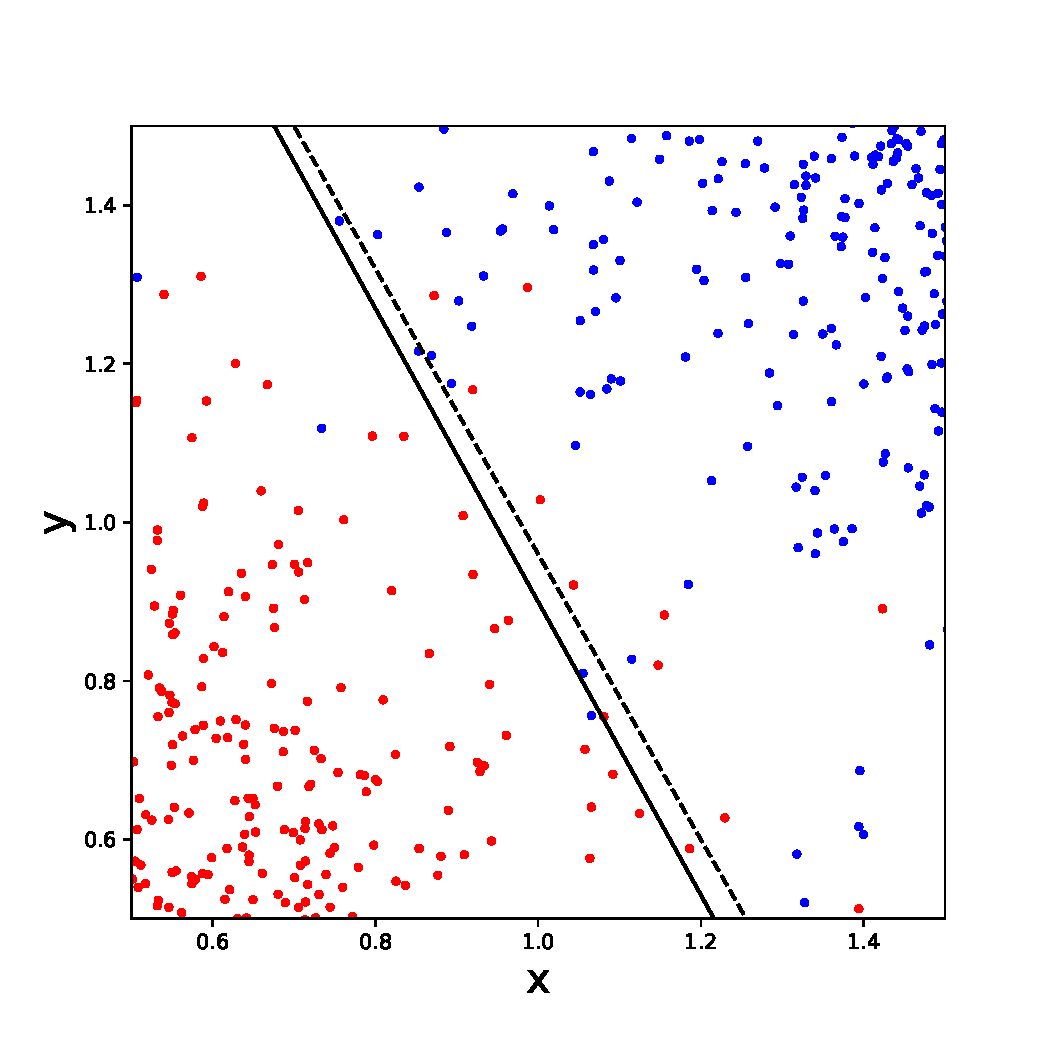
\includegraphics[width=0.7\textwidth]{jump.pdf}
  \end{center}
  \caption{Continuous changes for the parameters $\boldsymbol{w}$ is equivalent to rotating and moving the line in a smooth manner. Whenever the decision
    boundary is crossed, however, $\mathcal{E}$ will jump discontinuously. The decision line for the solid line is: 1.85x + y = 2.75, for the dashed line
    by: 1.8x+y = 2.76. This small change causes four points to be classified differently. Each time a line that moves from the solid line into dashed one and crosses
    a red point, the error functions jumps. It does not matter how smoothly the transition is made.
  }
\end{figure}

This becomes obvious if one realises that $\mathcal{E}$ essentially counts the number of misclassifications. When the decision boundary is changed smoothly it may cross
over a point that previously had been misclassified and is now classified correctly. The loss function $\mathcal{E}$ jumps. It is clear that $\mathcal{E}$ is not
a continuous function of the weights for the classical perceptron. This makes it hard to write down conditions on $\boldsymbol{w}$ that minimise $\mathcal{E}$ and nearly
impossible to use numerical methods such as \emph{steepest gradient descent}.

\begin{figure}
  \begin{center}
    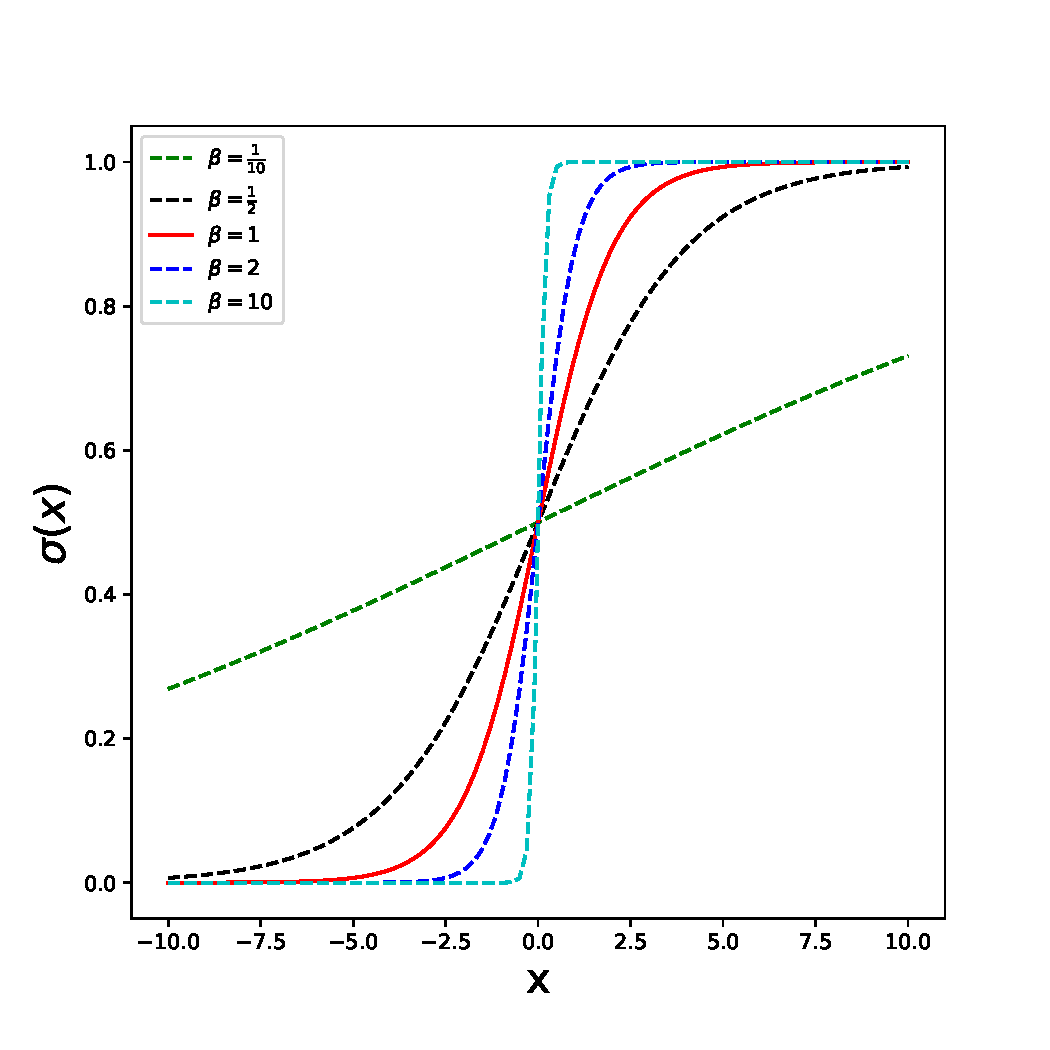
\includegraphics[width=0.7\textwidth]{sigmoid.pdf}
  \end{center}
  \caption{The logistic function for various values of the noise parameter $\beta$. Observe that for high values of $\beta$ the function
  resembles a step function.}
  \label{fig-logistic}
\end{figure}

At heart the cause of this problem is the use of the Heaviside function, which
is discontinuous in $x=0$. One way of avoiding it, is to replace by a smooth function.
Several such functions have been used in the past, including the logistic
function:
\begin{equation}
  \sigma(x) = \frac{1}{1+ e^{-\beta x}}
  \label{eq-logistic}
\end{equation}
In the following we will use $f(x)$ for an arbitrary squashing function, whose exact form we will determine later. $\sigma(x)$ will
always determine the logistic function (Eq. \ref{eq-logistic}).

The logistic function can be considered a soft version of the step function. This
means that a perceptron using  it will no longer make a hard decision, but one that
depends continuously on the input function. The 'hardness' of the decision
can be influenced with the choice of parameter $\beta$, which is sometimes
called a noise parameter.  Figure \ref{fig-logistic} demonstrates that high values
of $\beta$ lead to a function $f(x)$ that almost is equivalent to a step function.
Low values  of $\beta$ leads to a function which is flat in a considerable interval
around zero input.

\begin{figure}[!ht]
  \begin{center}
    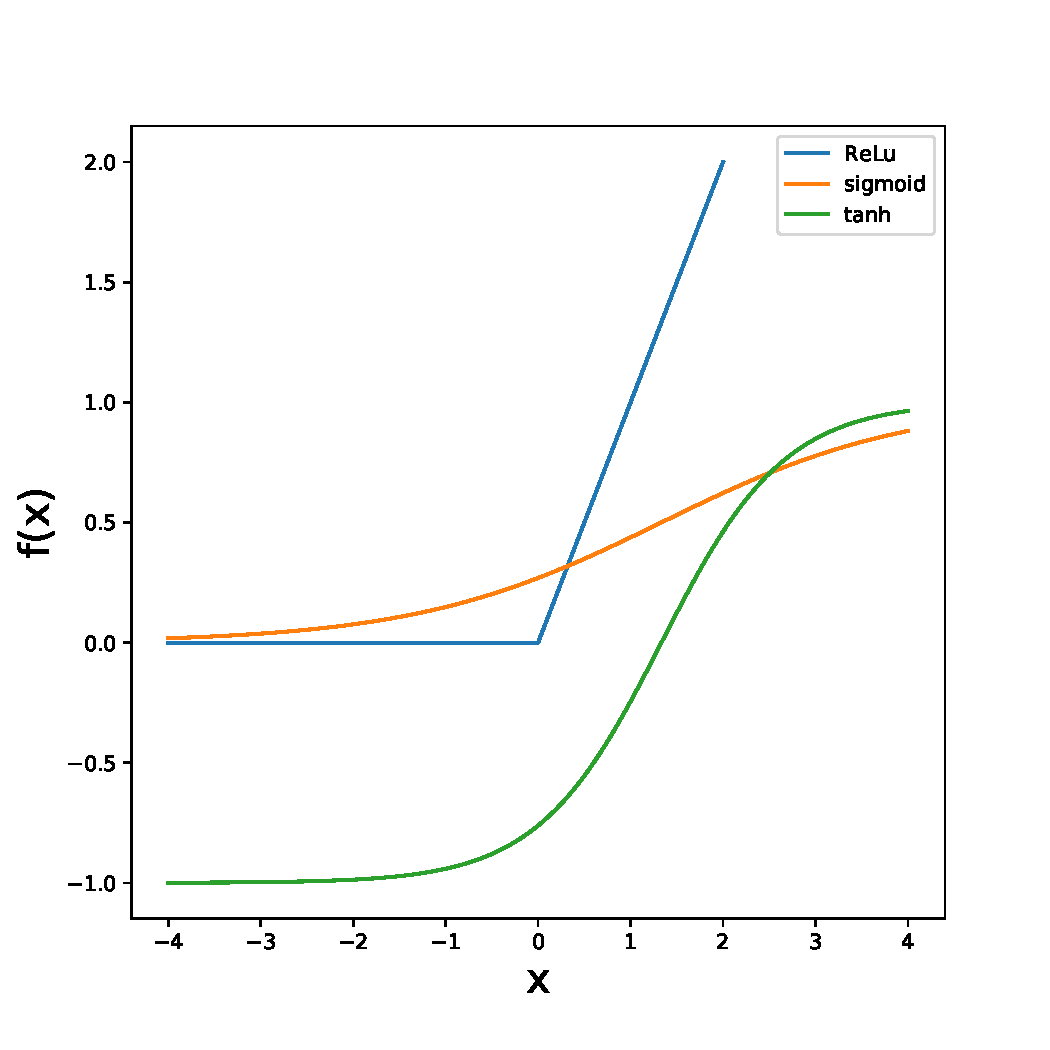
\includegraphics[width=0.7\textwidth]{relu.pdf}
  \end{center}
  \caption{Examples of squashing functions that are commonly used in neural networks. They all contain a non-linearity, which
    is essential in multi-layer perceptrons.}
  \label{fig-relu}
\end{figure}

Another function that has been popular with very
similar properties is tangent hyperbolic:
\begin{equation}
  f(x) = \frac{e^x - e^{-x}}{e^x + e^{-x}}
  \end{equation}
It looks similar to the logistic function, but has the interval $[-1, 1]$ as a range
whilst the logistic function has range $[0,1]$. Moreover the tangent hyperbolic
is anti-symmetric in its input. It maps 0 to 0, unlike the logistic function, which maps 0 to 0.5.
Because of their s-shaped form, these functions are sometimes called \emph{sigmoids}.

The function $f(x)$ are sometimes called \emph{squashing functions} because they compress the
input, which theoretically can be in the range $(-\infty,\infty)$ to a smaller, often finite
range. ReLu, or rectified linear unit, nowadays has become quite popular is shown
in Fig. \ref{fig-relu}.

All of the functions are continuous and almost every where differentiable. This has the important
consequence that the condition for minimisation of the loss function
can now be written down:

$$
\frac{\partial \mathcal{E}}{\partial \boldsymbol{w} } = 0
$$

Let us work this out for the logistic squashing function. We need to apply the chain rule:
\begin{equation}
  \frac{\partial \mathcal{E}}{\partial \boldsymbol{w}} = \sum_i (o_i - d_i) \frac{\partial}{\partial \boldsymbol{w}} o_i.
  \label{eq-part}
\end{equation}

Since
$$
o_i = \sigma(\boldsymbol{w}^T \boldsymbol{x}_i),
$$
so that
$$
\frac{\partial}{\partial \boldsymbol{w}} o_i = \sigma^{\prime}(\boldsymbol{w}^T \boldsymbol{x}_i) \frac{\partial \boldsymbol{w}^T \boldsymbol{x}_i}{\partial \boldsymbol{w}}
$$
When we write out $\boldsymbol{w}^T \boldsymbol{x} = \sum_j w_jx_j$, it is easy to see that
$$
\frac{\partial}{\partial w^i} \sum_j w^jx_j = x_i,
$$
or in vector notation:
$$
\frac{\partial}{\partial \boldsymbol{w}} \boldsymbol{w}^T \boldsymbol{x} = \boldsymbol{x} 
$$
Substituting this back into Eq. \ref{eq-part} gives:
$$
\frac{\partial}{\partial \boldsymbol{w}} o_i = \sigma^{\prime}(\boldsymbol{w}^T \boldsymbol{x}_i) \boldsymbol{x_i}
$$
Now, for the logistic equation, it is easy to show that
\begin{equation}
  \sigma^{\prime}(x)= \sigma(x)(1 - \sigma(x))
  \label{eq-prime}
\end{equation}
This very elegant property means that once you have calculated $\sigma(x)$ for a given value of $x$, calculating the derivative is
a simple multiplication! This means that the condition for minimising the loss function can be written as:
$$
\frac{\partial}{\partial \boldsymbol{w}} \mathcal{E} = \sum_i (\sigma(\boldsymbol{w}^T \boldsymbol{x}) - d_i)\sigma(\boldsymbol{w}^T \boldsymbol{x})( 1- \sigma( \boldsymbol{w}^T \boldsymbol{x} )) \boldsymbol{x}_i = 0
$$

This is a non linear system of equations - the $\boldsymbol{w}$ appear in the function argument of $f(x)$, which is a non linear sigmoid - and no analytic
techniques for solving them are available. We therefore have to resort to numerical techniques. We are faced with the problem
of function minimisation. An often used technique is \emph{steepest gradient descent}.

\section{A Learning Rule for the MSE Loss Function}

Imagine a function $\mathcal{E}(\boldsymbol{w})$,
which we aim to minimise, but if the function is non linear, it is almost always difficult to find algebraic conditions. However,
we usually can calculate the \emph{gradient} $\frac{\partial \mathcal{E}}{\partial \boldsymbol{w}} \mid{\boldsymbol{w}_0}$ in some point $\boldsymbol{w}_0$.
  It is important to realise that the represents a direction (i.e. a vector) in weight space. Now consider that we move away from the point $\boldsymbol{w}_0$
  in a direction given by a vector whose direction is unconstrained, but whose magnitude is fixed to a small value $h$. Depending on the direction,
  the function $\mathcal{E}$ will have a new value, $\mathcal{E}(\boldsymbol{w} + \boldsymbol{h})$. Calculus tells us that the gradient is \emph{the direction of maximum change}.
  If we are not at a maximum, a small step in the direction of the gradient will lead to a higher value of $\mathcal{E}$. Conversely, stepping against the gradient
  will lead to a lower value of $\mathcal{E}$. Steepest gradient descent consists of repeatedly make small moves in the direction of the negative gradient. When repeated
  often enough, one may arrive at a minimum or a saddle point. The saddle point can usually be avoided, by means explained below. Steepest gradient descent
  will find generally find a \emph{local} minimum. 

  In general, steepest gradient can be expressed as:
  \begin{equation}
    \boldsymbol{w} \rightarrow \boldsymbol{w} - \lambda \frac{\partial \mathcal{E}}{\partial \boldsymbol{w}}
    \label{eq-steepest}
  \end{equation}
  Here $\lambda$ is called the \emph{learning rate}. Theory sets no other constraints than that it be 'small'. Its choice in practice will have to be determined
  by experimentation. Too small and convergence to a minimum takes a long time, too large and it may overshoot the minimum. When $\lambda$ has been chosen
  appropriately, repeated application of Eq. \ref{eq-steepest} will lead to a set of weights for which the loss function is locally minimal.
  Eq. \ref{eq-steepest} is an example of a \emph{learning rule}, an iterative algorithm that uses parts of a dataset to improve weights for classification.
  
  Given that we already have evaluated the gradient of the loss function for the case of a logistic squashing function, we can immediately write down the
  the steepest gradient descent rule:

  \begin{equation}
    \boldsymbol{w} \rightarrow \boldsymbol{w} - \lambda \sum_i o_i(1-o_i)(d_i - o_i) \boldsymbol{x}_i
    \label{eq-delta}
  \end{equation}
  This is sometimes written as
  $$
  \boldsymbol{w} \rightarrow \boldsymbol{w} - \lambda \sum_i \Delta_i x_i,
  $$
  with
  $$
  \Delta_i \equiv o_i ( 1- o_i) (d_i - o_i).
  $$

  \emph{This is not a great learning rule, certainly not for classification problems.} We will look at improvements below.
  One reason is immediately obvious: the desired classification
  is either '0' or '1', but once the weights start to approach values such that the perceptron starts to produce these values, learning slows down,
  due to the factor $o_i(1 - o_i)$, which approaches 0 if $o_i$ starts to approach 0 or 1.  Nevertheless, the example is important.
  Here, we have seen the first example of how steepest gradient descent is employed to minimise a loss function. Apart from an overall constant, this loss
  function is equivalent to the  Mean Squared Error (MSE) loss function that we already encountered in Unit 1.

  Note that for the problem at hand, classification of data points into two classes, this learning rule is the perceptron rule in disguise. 
  
  The perceptron learning rule essentially states that the weights should not be changed if classification is correct, that the weights should be changed
  in the direction of the input if the desired classification is '1' and current classification is '0', and away from the input in the opposite case.
  If it were not for the the factor $o_i(1-o_i)$, Eq. \ref{eq-delta} states the same thing. But the factor $o_i(1 - o_i)$ changes the magnitude of the
  correction to the weights, not its direction, which is in the direction of the input factor. And since the magnitude can be manipulated by the
  learning rate $\lambda$,  Eq. \ref{eq-delta} is not very different from the perceptron algorithm with a learning rate.

  \begin{figure}
    \begin{center}
      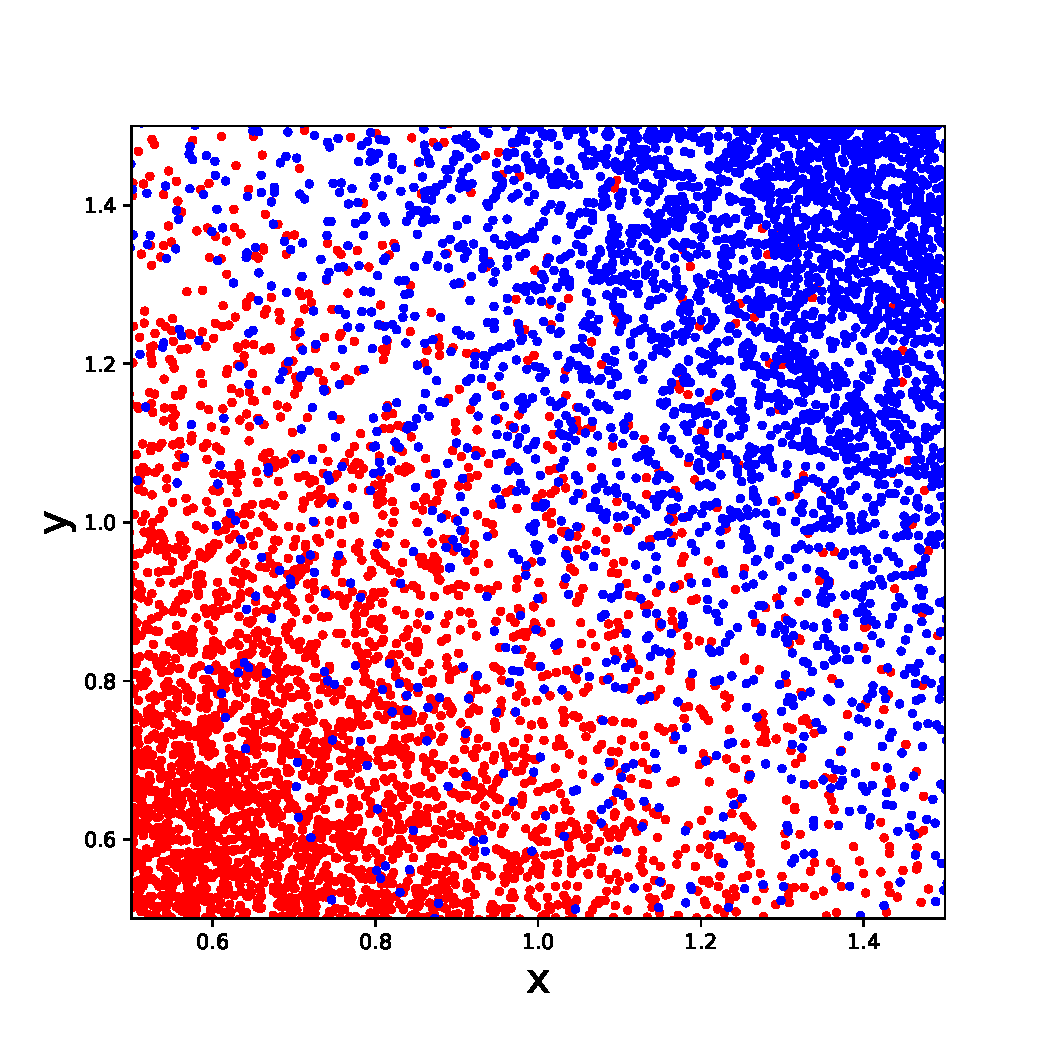
\includegraphics[width=0.7\textwidth]{almost.pdf}
    \end{center}
    \caption{A data classification problem where a linear classifier is a reasonable solution, although technically the dataset is not linearly separable.}
    \label{fig-almost}.
  \end{figure}
  
  The approach presented here, steepest gradient descent nevertheless represents an  improvement over the classical perceptron algorithm in two important ways.
  \begin{enumerate}
  \item The classical perceptron algorithm cannot handle data that is not linearly separable. It will just loop forever. There are genuinely
    complex classification problems that a single perceptron cannot be expected to handle. But consider the classification problem shown in
    Fig. \ref{fig-almost}. A linear classifier would be appropriate, but the original perceptron algorithm cannot handle it.

  \item The perceptron algorithm just stops when it finds a set of weights that work. It does not try to find the 'best' weights in any
    sense.
  \end{enumerate}

  By using a steepest gradient descent version of the algorithm, these problems are alleviated. First, one can \emph{monitor} the performance of the algorithm by
  occasionally evaluating the loss function for the current set of weights. This makes it possible to create a \emph{stopping criterion}. For linearly
  separable data one immediately stops when the loss function is zero. For non linearly separable data the loss function can never become zero,
  but  it will typically start to hover around a small value, at least smaller than for a purely random set of weights. A little experimentation can give
  a sense for what a good stopping value is. In a non linearly separable dataset the stopping criterion ensures that the solution if not perfect, is at least reasonable.


  \subsection{Batches, Minibatches and Momentum }
  \begin{figure}[!ht]
    \begin{center}
      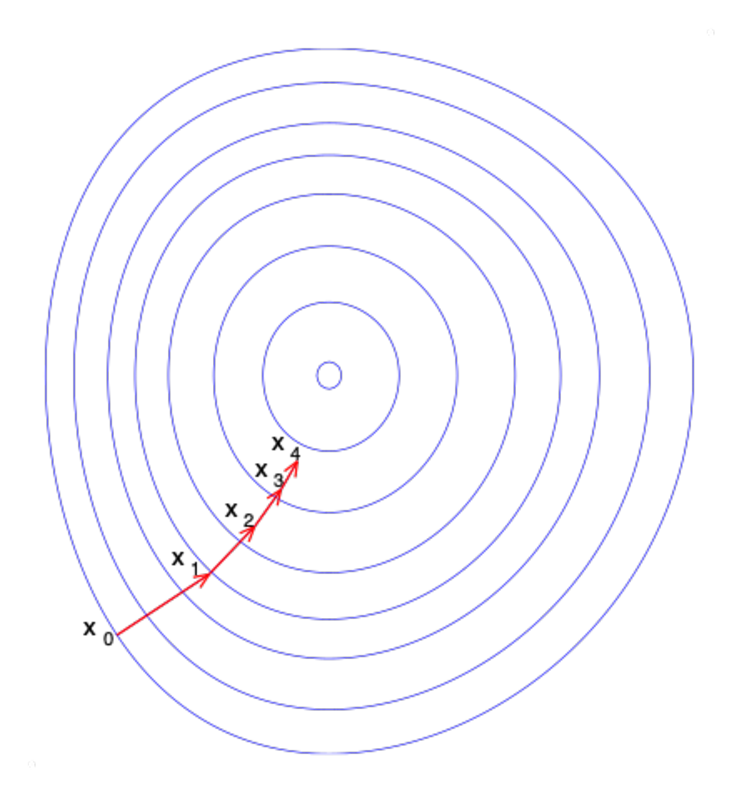
\includegraphics[width=0.7\textwidth]{Gradient_descent.pdf}
    \end{center}
    \caption{Steepest gradient descent in a favourable loss landscape. Source: Wikipedia}
    \label{fig-sgdgood}
  \end{figure}

  In the steepest gradient descent version of the algorithm the gradient was calculated over the entire dataset. Although correct according to calculus, this is
  usually not the most efficient way of training a neural network. The gradient only tells you what \emph{locally} is the best way to go in weight space, but how the
  algorithm performs depends on the entire landscape in weight space.
  
  For a linearly separable dataset the perceptron theorem informs us that there is a \emph{global} minimum of the loss function. After all, a set of weights exists that
  allow for no misclassifications at all. Also, there are no local minima. This is also plausible if we look at Fig. \ref{fig-almost}. It is clear that whenever we
  move the decision boundary to another position, overall the number of misclassifications increases. We can think of this loss landscape as being concave, and since
  the loss function is quadratic in the weights, its contours resemble an ellipsoid like in  Fig. \ref{fig-sgdgood}.


  So, in this case steepest gradient descent is guaranteed to find the minimum. However, even though there is a quadratic minimum, this is not necessarily
  spherically symmetric, but the minimum may be quite elongated. In that case, the local gradient may not point in the direction. 

  \begin{figure}[!ht]
    \begin{center}
    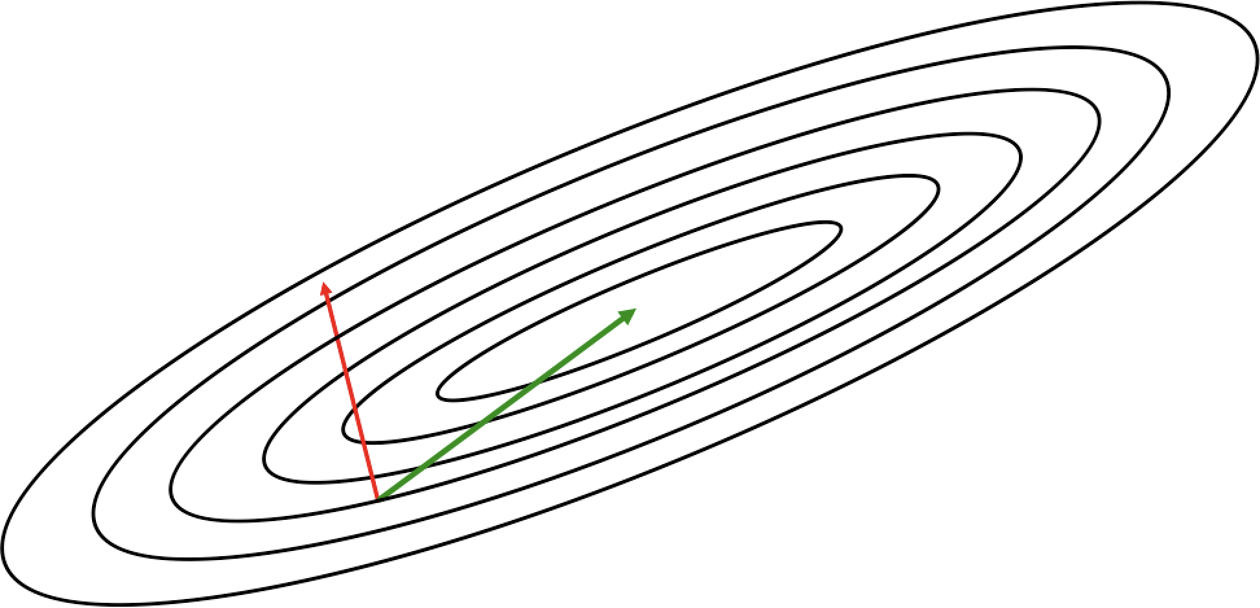
\includegraphics[width=0.7\textwidth]{fodl_0406.png}
    \end{center}
    \caption{An elongated minimum may lead to slow convergence of steepest gradient descent, because the gradient does not really point to the minimum (left).}
    \label{fig-elong}
  \end{figure}

  This may lead to a very slow convergence. Ideally, steepest gradient descent should traverse the contours of the loss landscape quickly, as shown in Fig. \ref{fig-sgdgood}.
  However, elongated shapes may lead to a zigzag course in the loss landscape, due to the gradient locally not pointing to the centre. An extreme example
  is shown in Fig. \ref{fig-bad}, where due to zigzagging the algorithm almost follows a contour in the landscape, which means it is converging extremely slowly.

  \begin{figure}
    \begin{center}
      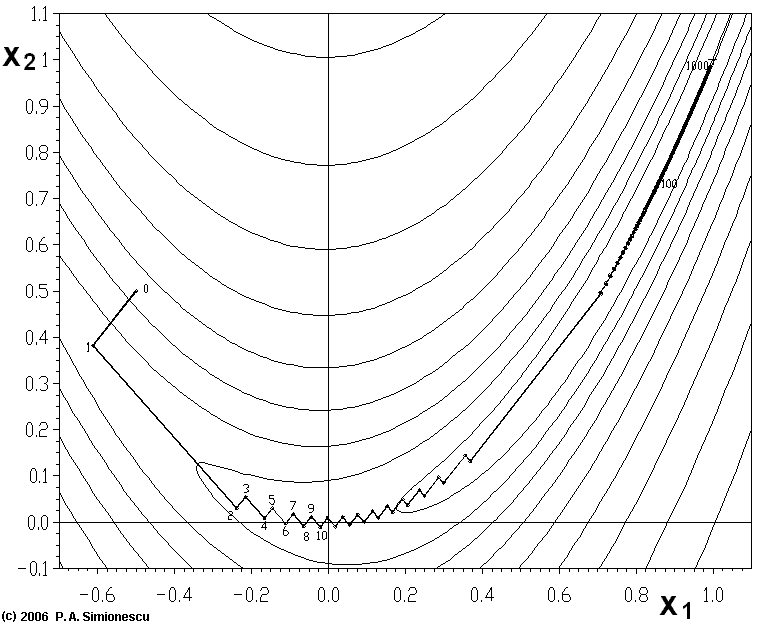
\includegraphics[width=0.7\textwidth]{Banana-SteepDesc.png}
    \end{center}
    \caption{Very slow convergence of steepest gradient descent, due to zigzagging (source Wikipedia).}
    \label{fig-bad}
  \end{figure}


  These problems are well known in the neural network literature. One strategy is not to use the entire training dataset in the calculation of the gradient, a procedure
  called \emph{batch training}, as the entire batch of training patterns is used. The other end of the spectrum is to calculate the gradient
  on single data points, which is called \emph{online learning}. If each data point is chosen randomly from the training set, this adds some random jittering
  to the direction of the descent, which is often useful in practice. Most neural network training adopts a strategy somewhat in  between. A number of $m$ patterns
  is selected, called a \emph{minibatch}. The gradient is then estimated over this batch. This approach is called \emph{stochastic gradient descent}.

  Another approach aiming to alleviate the zigzagging is to use \emph{momentum}. When using momentum, the gradient that was calculated in a previous iteration
  of the algorithm is saved. In the current iteration the gradient is calculated again, but the change implemented of the weights is a weighted
  average of the 'old' and the 'new' gradient. Symbolically, the learning rule can be represented as follows:

  \begin{equation}
  \Delta  \boldsymbol{w}_{t} =  - \lambda \frac{\partial \mathcal{L}}{\partial \boldsymbol{w}} + \alpha \Delta \boldsymbol{w}_{t-1}
  \end{equation}
  Here $\Delta \boldsymbol{w}_t$ is the current change of weights. Without momentum term ($\alpha = 0$), this is steepest gradient descent as usual.
  
  Momentum and stochastic gradient descents are two examples of optimising. There is a large number of optimisation techniques, too large to cover here. Before you
  start training neural networks in anger, you should consult a recent review of modern optimisation techniques, for example Chapter 8 of \cite{goodfellow2016}.

  \chapter{Logistic Regression}
\section{Logistic Regression: Discriminative Modelling}
\label{eq-logdisciminative}
In Sec. \ref{sec-percloss} we have provided the historical argument for a perceptron with a soft decision function, which happened to be the logistic function, which
was in fact selected for its neat algebraic properties, in particular the fact that the derivative can be calculated by simple multiplication when
the function value is  known (Eq. \ref{eq-prime}). This leads to elegant expressions for learning rules but not always to efficient learning.

Logistic regression does not use a hard decision function to make a decision, but models the probability of an outcome instead. The sigmoid function, which we reproduce for
convenience in Fig. \ref{fig-logistic2} is suitable for this interpretation.

\begin{figure}
  \begin{center}
    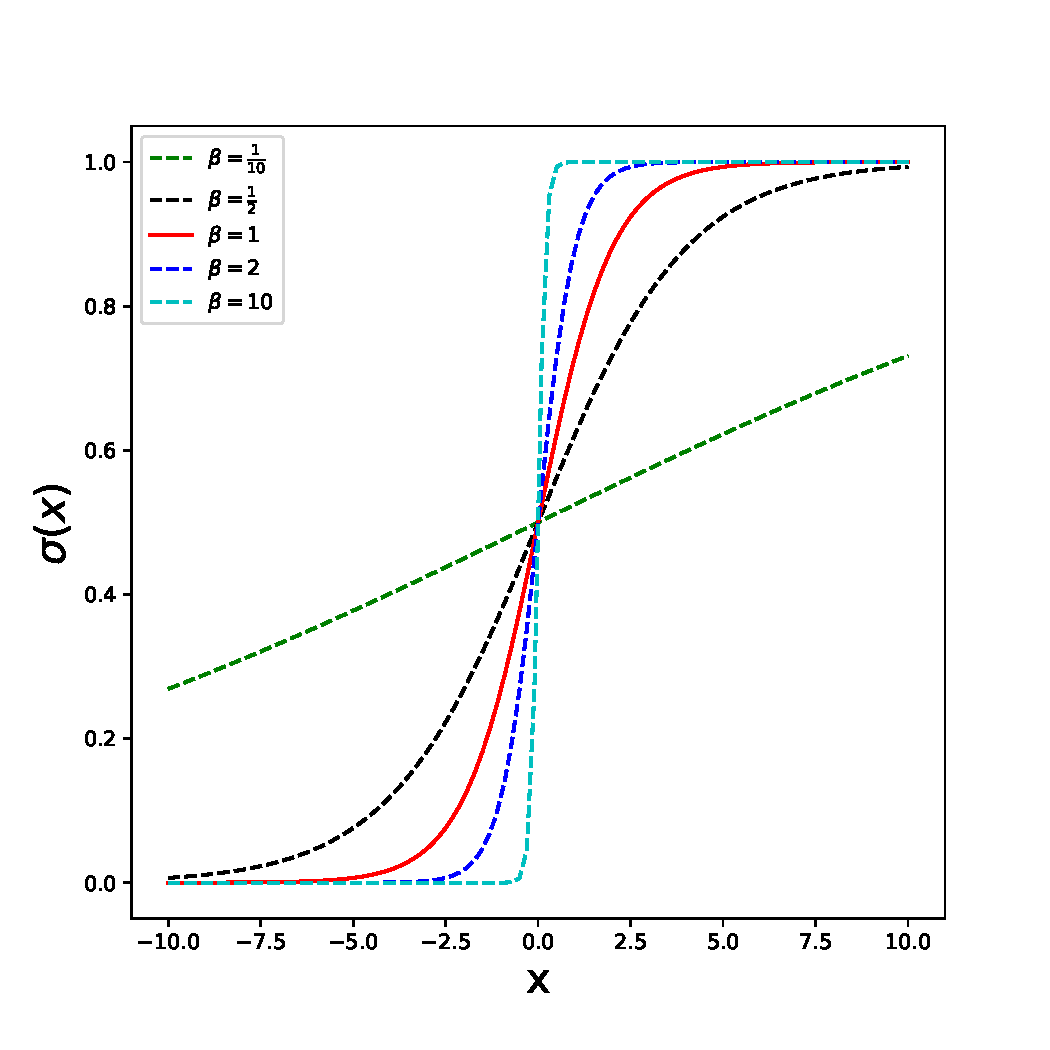
\includegraphics[width=0.7\textwidth]{sigmoid.pdf}
  \end{center}
  \caption{The logistic function for various values of the noise parameter $\beta$. Note that because the output is between 0 and 1, it can be interpreted as a probability.}
  \label{fig-logistic2}
\end{figure}


The definition of a logistic regression classifier is now given by:
$$
p(\mathcal{C}_1 \mid \boldsymbol{\phi}) = \sigma(\boldsymbol{w}^T \boldsymbol{\phi}),
$$
with
$$
\sigma(x) = \frac{1}{1 + e^{-x}}
$$
and our task is to find weights that produce the best classification possible.


To this end, we define a likelihood function. Let the dataset be $\{ \phi_i, t_i \}$ with $\phi_i = \phi(\boldsymbol{x}_i)$ and $t_i \in \{ 0, 1 \}$. The labels
$t_i$ are given: the dataset is \emph{labelled}. Writing $\boldsymbol{t}$ for $(t_1, \cdots t_N)$ we write:
\begin{equation}
  p(\boldsymbol{t} \mid \boldsymbol{w}) = \Pi^N_{i=1} y^{t_i}_i ( 1 - y_i)^{1 - t_i},
  \label{eq-logllh}
\end{equation}
where $y_i = p(\mathcal{C}_1 \mid \phi_i) = \sigma(\boldsymbol{w}^T \boldsymbol{\phi}(\boldsymbol{x})_i)$.

In line with our experiences from Unit 1, this formula simplifies when we consider the  log likelihood:
\begin{equation}
\mathcal{E}(\boldsymbol{w}) = \ln p(\boldsymbol{t} \mid \boldsymbol{w} ) = \sum^N_{i=1} t_i \ln y_i + (1 - t_i) \ln ( 1 -  y_i) 
\label{eq-cross}
\end{equation}

This is again  an error or a loss function, as the set of $\boldsymbol{w}$ that minimises it  minimises prediction loss.
Minimising this function with respect to $\boldsymbol{w}$ is equivalent to maximising the likelihood function. 
In line with our approach so far, we can calculate the gradient and perform steepest or stochastic gradient descent:

\begin{equation}
  \frac{\partial \mathcal{E}}{\partial \boldsymbol{w}} = \sum^N_{i=1}(y_i - t_i)\phi_i
  \label{eq-crossgrad}
\end{equation}

%{\noindent Exercise: Show this}.\\
This is a nice and tidy result. It is similar to the perceptron learning rule, note that we wrote $o_i$ there, instead of $y_i$. We maintain the distinction, reflecting
that $o_i$ is traditionally used in the Connectionism literature, and $y_i$ in machine learning but they both refer to the quantity:
$$
\sigma( \boldsymbol{w}^T \phi_i).
$$
If we compare the two rules, there no factor $o_i(1 - o_i)$ here. This is due to the difference in loss functions Eq. \ref{eq-mse} and \ref{eq-cross}.
It is worthwhile commenting on the difference. Let us recall the definition of the Kullback-Leibler divergence from Unit 1.
\begin{equation}
\mbox{KL}(p \mid \mid q) = - \int p (\boldsymbol{x}) \ln q (\boldsymbol{x} ) d \boldsymbol{x} -( - \int p(\boldsymbol{x}) \ln p( \boldsymbol{x}) d \boldsymbol{x})
\label{eq-KL}
\end{equation}
For a discrete probability distribution this works out as:
$$
\sum_{i \in C_i} p_i \ln q_i + \sum_{i \in C_i} p_i \ln p_i 
$$
The sum here is over the different outcomes and their probabilities - it is not a sum over events. The first term of this sum is the \emph{cross entropy}, the second
one is (self)-entropy. For the two class outcomes $\mathcal{C}_1$ and $\mathcal{C}_2$, with probabilities $p_1$, and $1-p_1$. The cross entropy of a probability distribution
with two outcomes is therefore:
$$
p_1 \ln q_1 + (1 - p_1) \ln (1 - q_1)
$$

We remember that the KL-divergence is a measure between probability, in this case a 'true' distribution $p_i$ and another distribution $q_j$. If we amend
the probability distribution $q_j$ in a way that reduces the KL-divergence, $q_j$ will be more than $p_i$ in a well defined manner. We can now recognise
Eq. \ref{eq-cross} as the cross entropy. Eq. \ref{eq-crossgrad} would allow us to design a gradient-based learning rule that ensure minimisation of the cross
entropy and thereby the KL-divergence, since the second term in the KL-divergence Eq. \ref{eq-KL} is a only function of the true distribution, which we use as reference.

  \section{Generative Models and the Logistic Function}
  \label{sec-generative}
  So far, have used a graded perceptron as a way for training a classifier that makes a hard decision. Devices that take a hard decision, based on
  which side of the hyperplane a data point lies are called \emph{discriminants}. However, a probabilistic interpretation of the sigmoid squashing function,
  which after all yields numbers between 0 and 1 leads to \emph{logistic regression}, an important statistical technique in its own right.


  Logistic regression arises naturally in the context of  \emph{probabilistic generative models} \citet{bishop2006}. Assume that we are generating a dataset
  where the points belong to one of two classes $\mathcal{C}_1, \mathcal{C}_2$, and that conditional probabilities $p(\boldsymbol{x} \mid \mathcal{C}_1)$ and
  $p( \boldsymbol{x} \mid \mathcal{C}_2)$  as well as  prior probabilities $p(\mathcal{C}_1), p(\mathcal{C}_2)$ are given. We can then  simulate a dataset:
  we first simulate a Bernoulli process to determine which of the two classes the point belongs to, and then we use the selected conditional probability
  to generate the point. For example, $\mathcal{C}_1$ might correspond to a genetic factor that influences the height distribution of mature individuals. Lacking this
  factor, individuals belong to a class $\mathcal{C}_2$, whose individuals may have a different height distribution.
  Often, $p(x\mid \mathcal{C}_1)$ , $p(x \mid \mathcal{C}_2)$ are known and we are faced with the problem of how likely it is that a given individual of height
  $x_i$ belongs to $\mathcal{C}_1$ or $\mathcal{C}_2$, when all the information we have available is the person's height. 

  Bayes' law gives an answer, since:
  \begin{equation}
    p(\mathcal{C}_1 \mid x) = \frac{p(x \mid \mathcal{C}_1) p(\mathcal{C}_1)}{p(x \mid \mathcal{C}_1) p(\mathcal{C}_1)+ p(x \mid \mathcal{C}_2) p(\mathcal{C}_2)}
  \end{equation}

  This can be rearranged to:
\begin{equation}
  p(\mathcal{C}_1 \mid x) = \frac{1}{1 + \exp(-a)},
  \label{eq-sigmoidemerge}
\end{equation}
with
\begin{equation}
  a = \ln \frac{p(x \mid \mathcal{C}_1) p(\mathcal{C}_1)}{p(x \mid \mathcal{C}_2) p(\mathcal{C}_2)}
  \label{eq-a}
\end{equation}
In Eq. \ref{eq-sigmoidemerge}, we see that the sigmoid function emerges quite naturally.

%A simple example: imagine that people who belong to $\mathcal{C}_1$ have a height distribution according to $\mathcal{N}(176,5^2)$ (they are 176 cm tall on average with
%a standard deviation of 5 cm). People who belong to $\mathcal{C}_2$ have a height distribution $\mathcal{N}(181, 5^2)$. In the overall population, the probability of belonging
%to class $\mathcal{C}_1$ = 0.75. Now we have someone in front of us who is 185 cm tall. It is seems more likely they belong to class $\mathcal{C}_2$, but by how much?
%Substituting the numbers gives a 13 \% probability of belonging to $\mathcal{C}_1$.


\begin{figure}[!ht]
  \begin{center}
    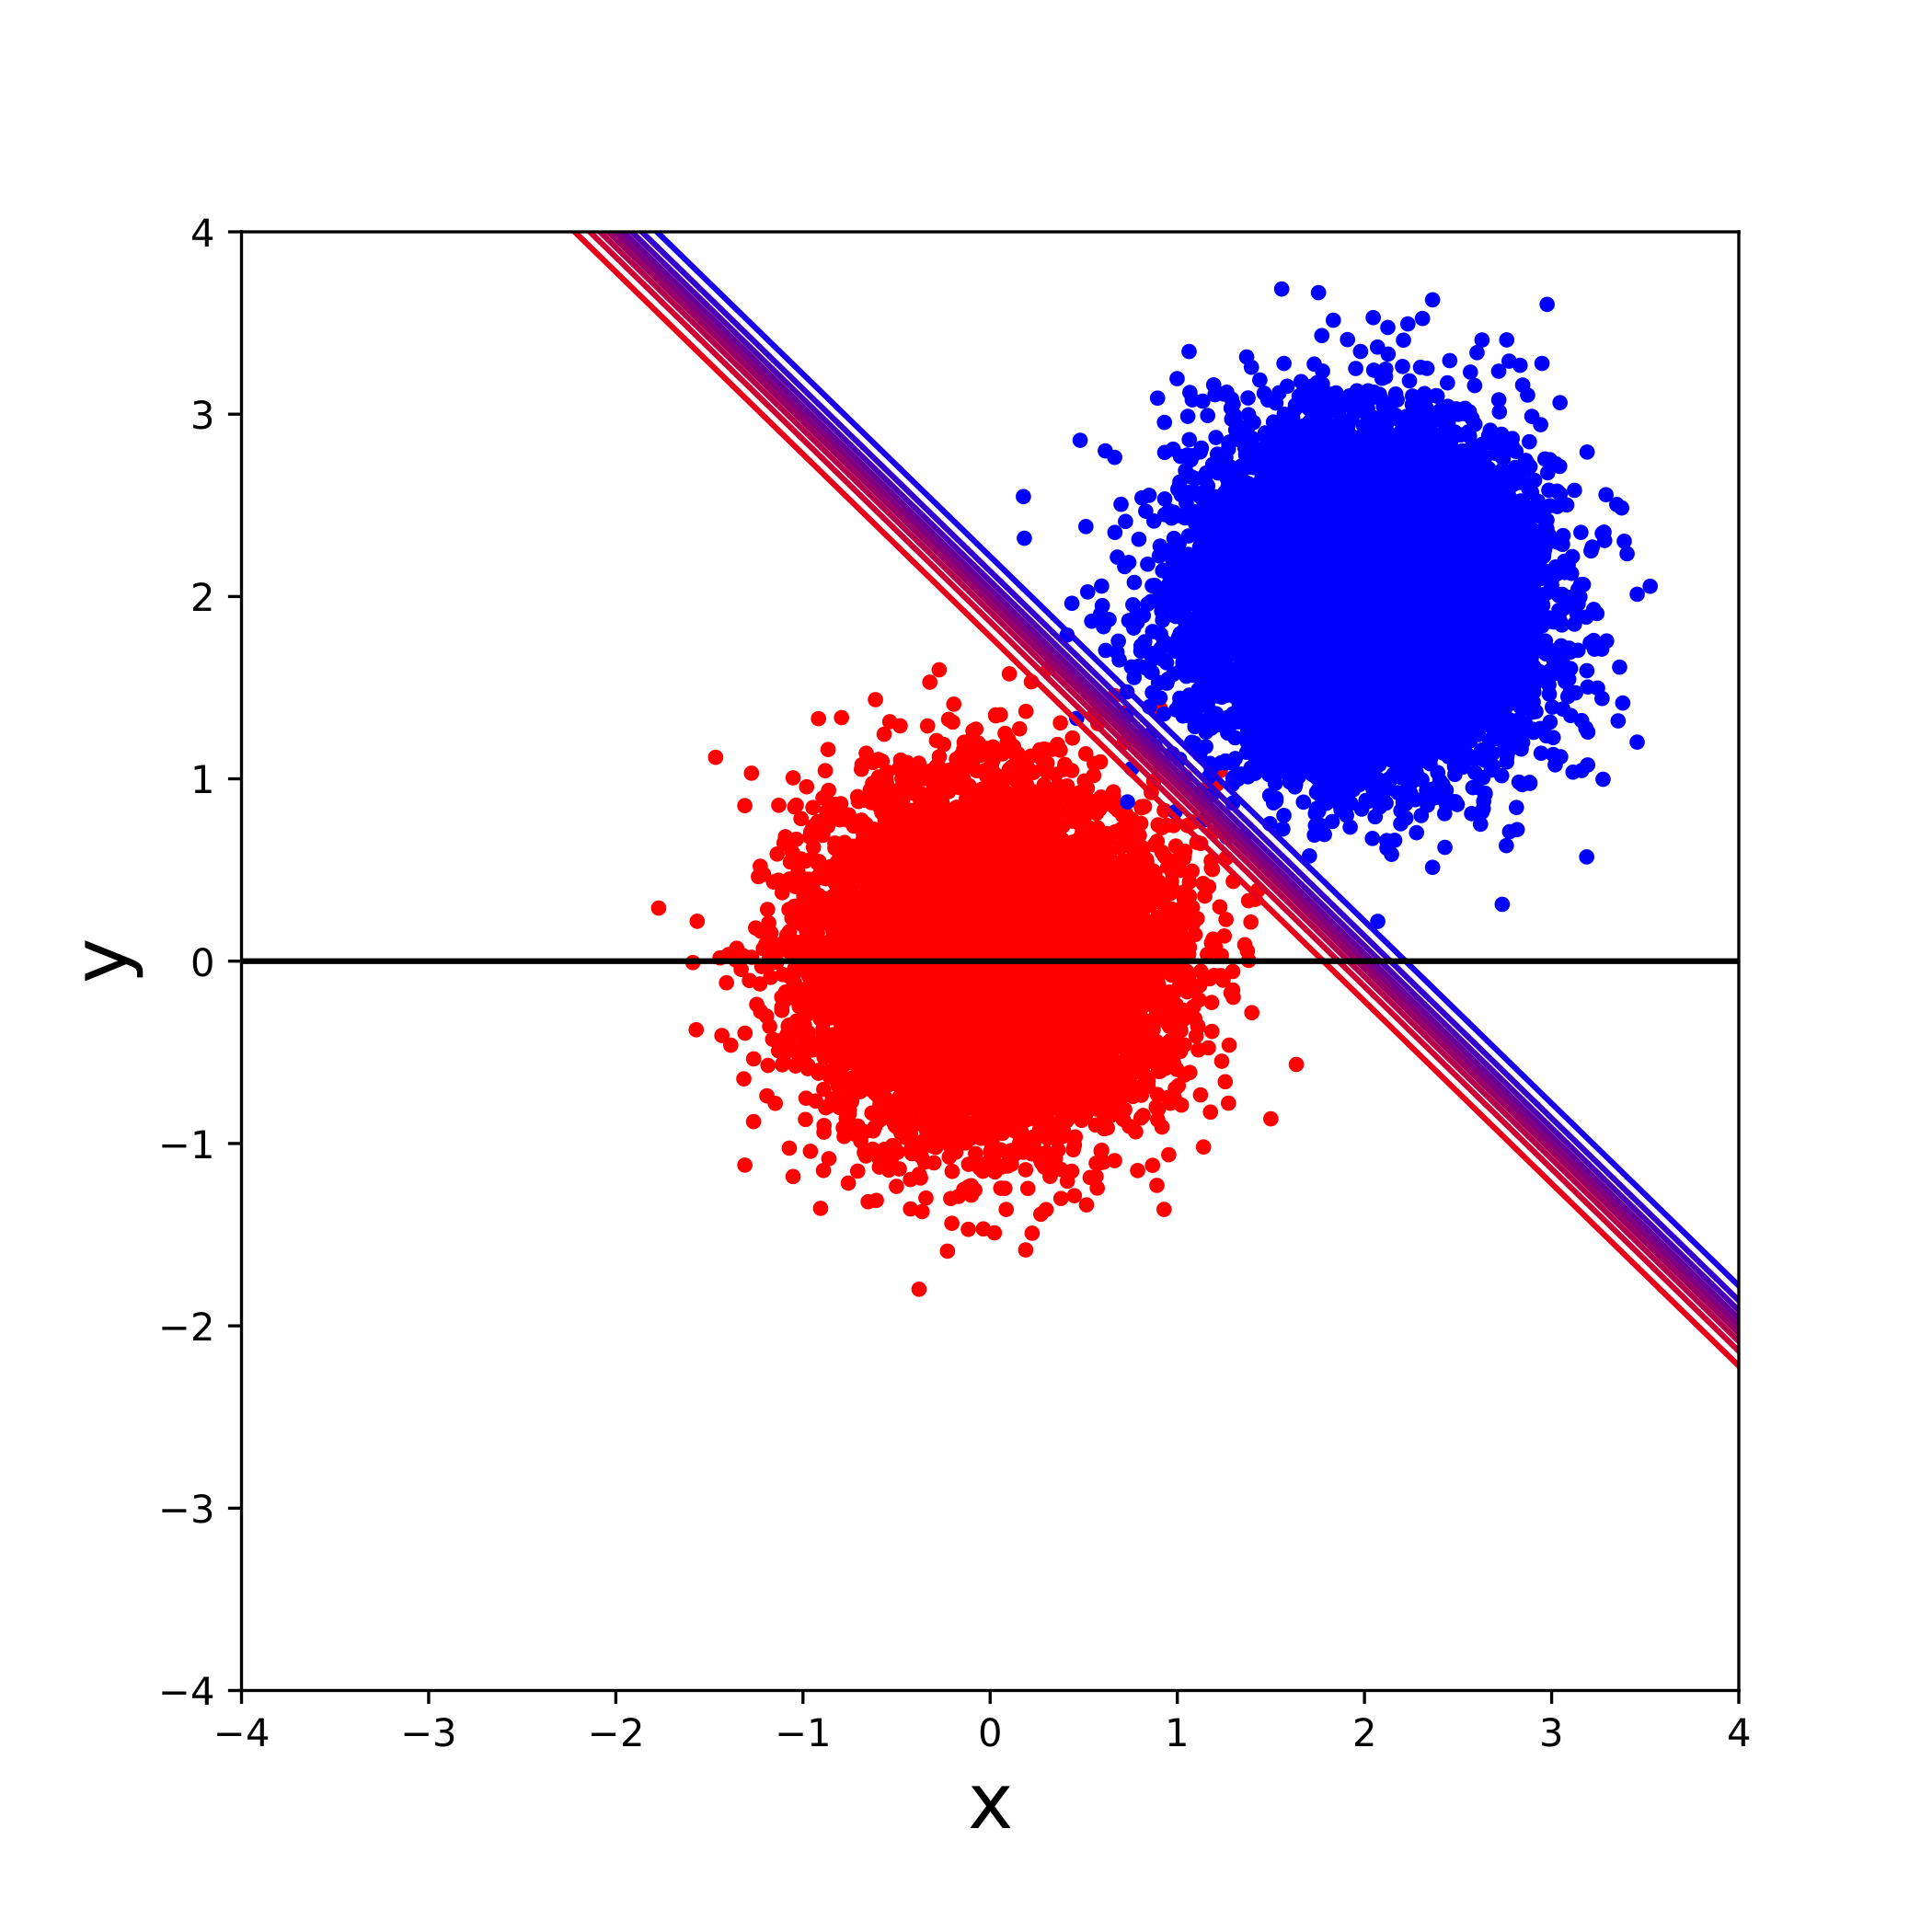
\includegraphics[width=0.35\textwidth]{sigmoidmotivation1.png}
    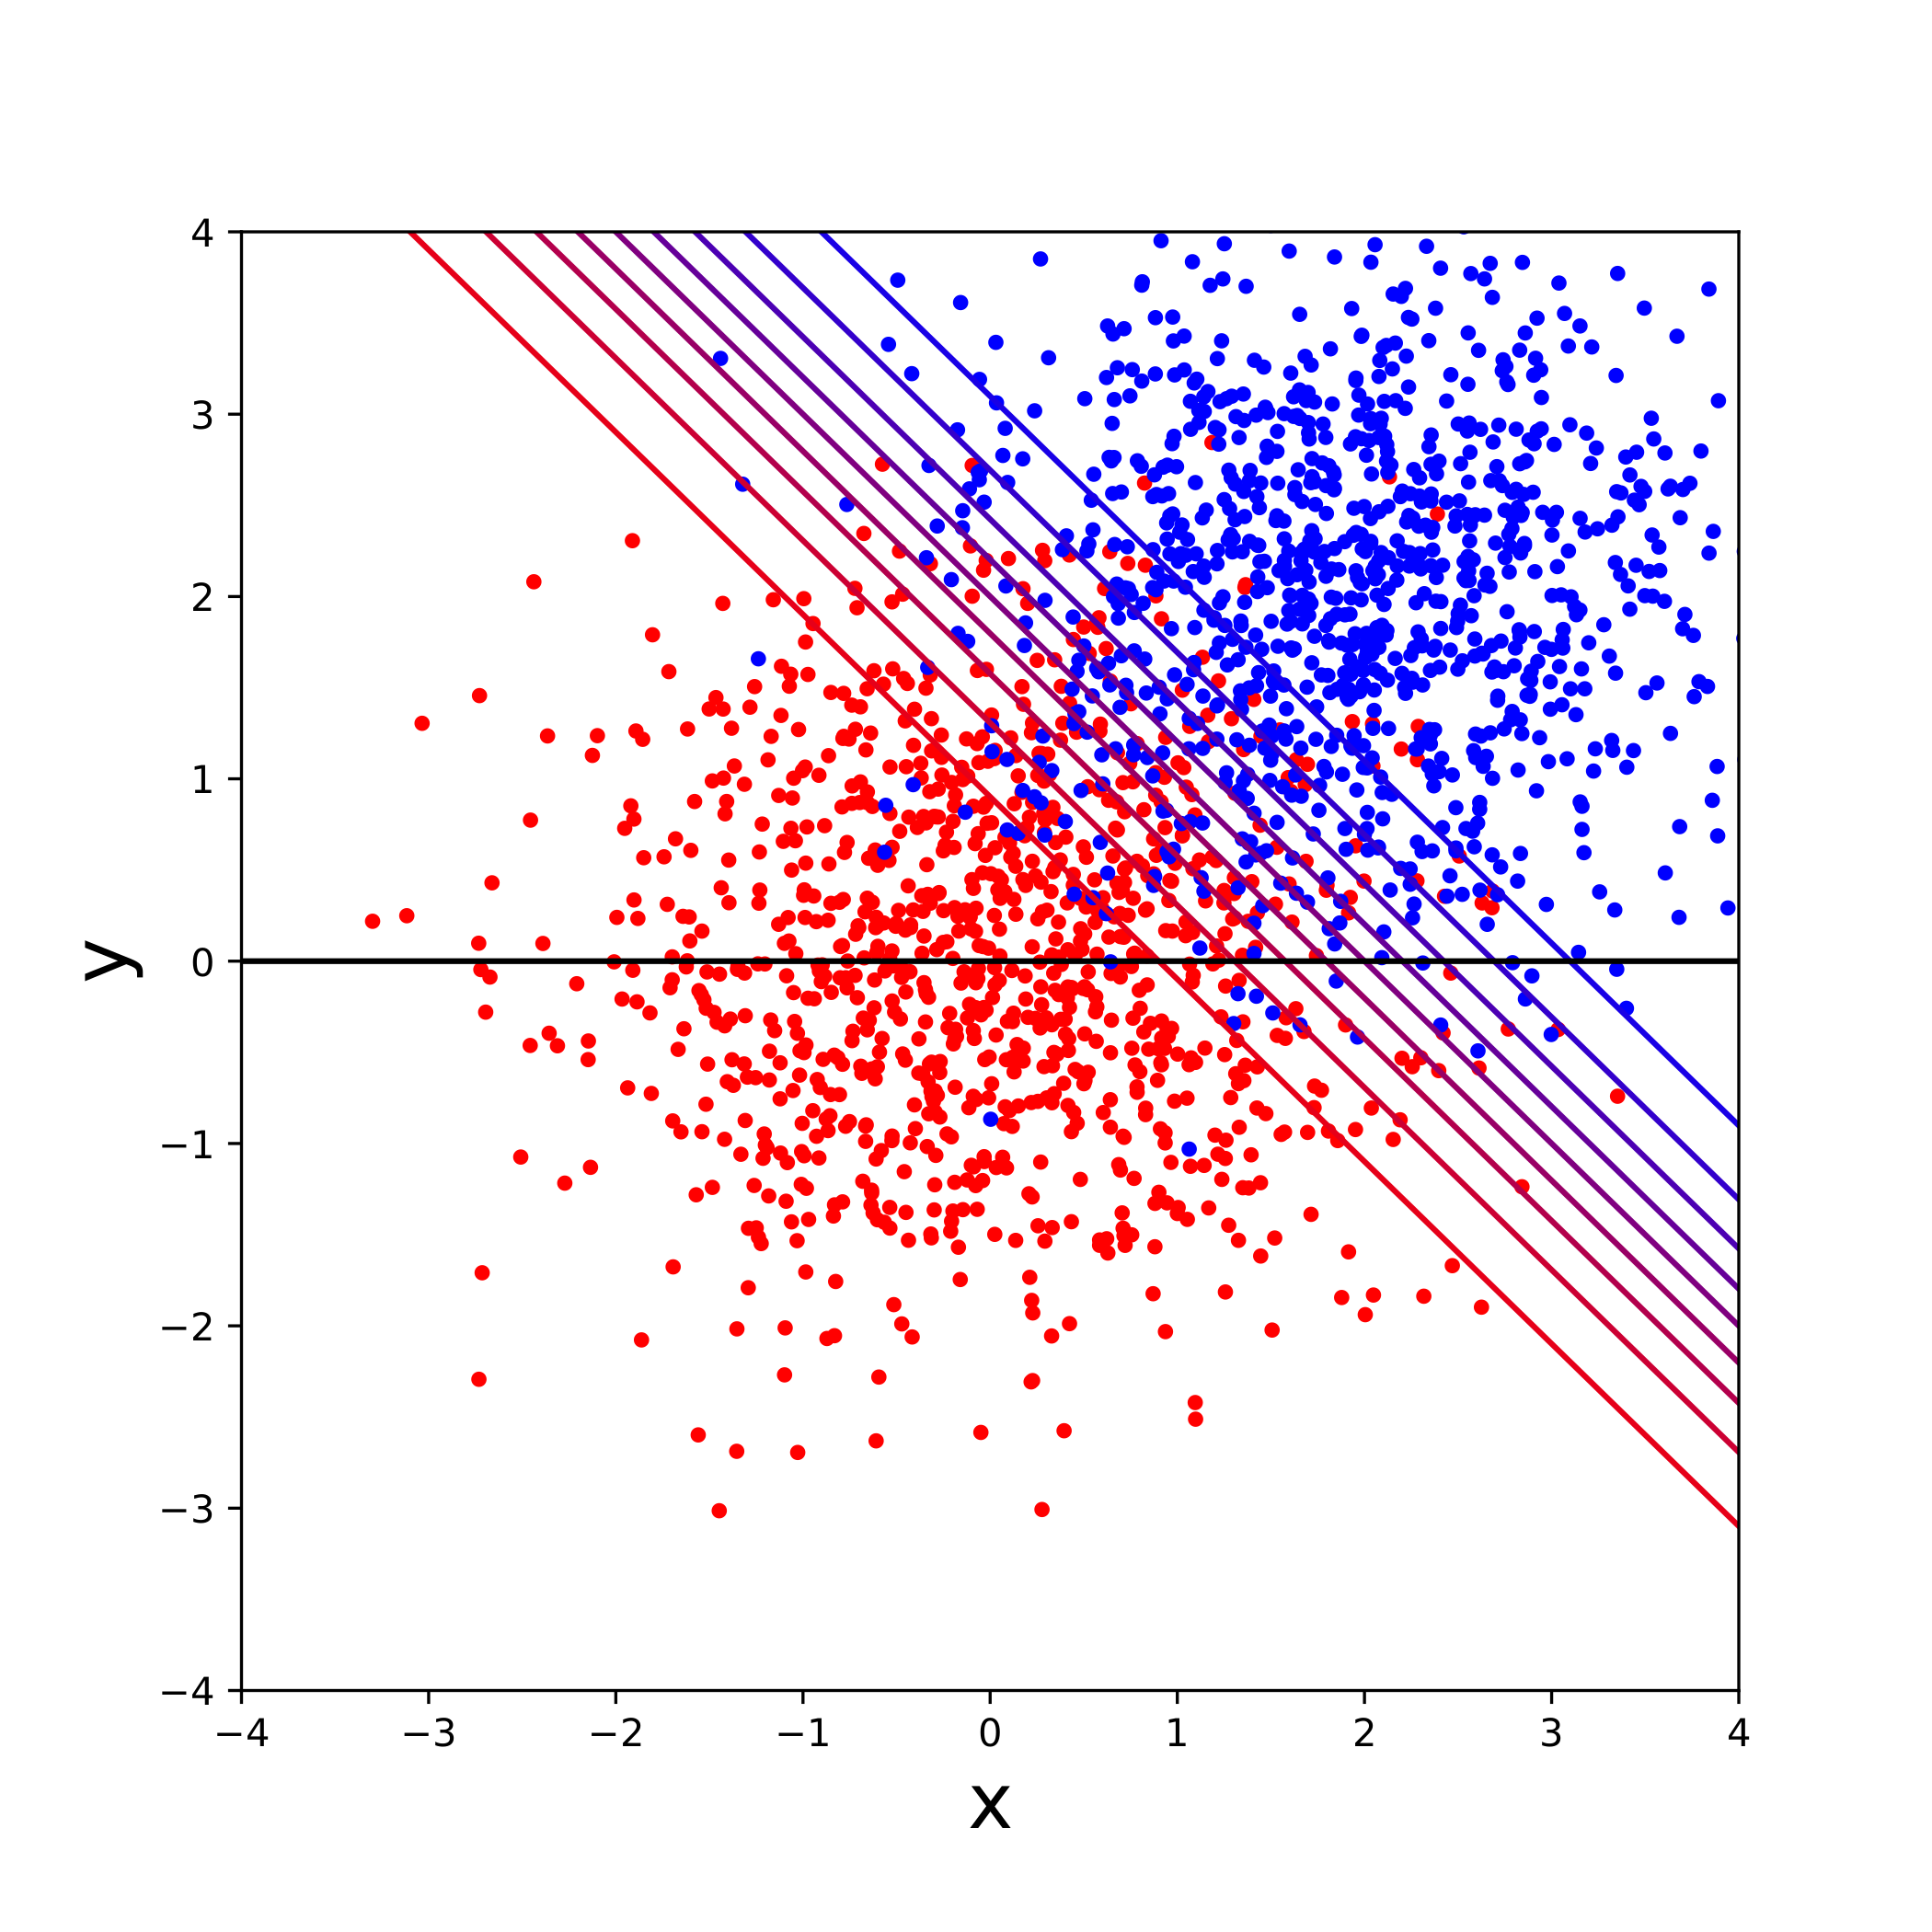
\includegraphics[width=0.35\textwidth]{sigmoidmotivation2.png} 
  \end{center}
     \caption{Two stochastic processes each generate data points that are Gaussian distributed. The red dots belong to class $\mathcal{C}_1$, the
       blue dots to class $\mathcal{C}_2$. Isolines for the probability $p(\mathcal{C}_1) = 0.1 \cdots 0.9$ (probability for a point being 'red') are given,
       calculated using Eq. \ref{eq-sigmoid2d}. When we restrict $x_2$ to 0 (black horizontal line), a one dimensional sigmoid emerges.}
    \label{fig-twoclass}
  \end{figure}


  As an example, consider Gaussian class-conditional functions:
  \begin{equation}
p\left(\mathbf{x} \mid \mathcal{C}_{k}\right)=\frac{1}{(2 \pi)^{D / 2}} \frac{1}{|\mathbf{\Sigma}|^{1 / 2}} \exp \left\{-\frac{1}{2}\left(\mathbf{x}-\boldsymbol{\mu}_{k}\right)^{\mathrm{T}} \boldsymbol{\Sigma}^{-1}\left(\mathbf{x}-\boldsymbol{\mu}_{k}\right)\right\}     
  \end{equation}


   A two-dimensional two class example is given in Fig. \ref{fig-twoclass}, where two Gaussian blobs are visible. When presented with a new data point $\boldsymbol{x}$,
   what is the probability that it belongs to class 1? From Eq. \ref{eq-sigmoidemerge} and \ref{eq-a} we find:
   \begin{equation}
     p(\mathcal{C}_1 \mid \boldsymbol{x}) = \sigma( \boldsymbol{w}^T \boldsymbol{x} + w_0)
     \label{eq-sigmoidlin}
   \end{equation}
   with:
   \begin{align}
\mathbf{w} &=\boldsymbol{\Sigma}^{-1}\left(\boldsymbol{\mu}_{1}-\boldsymbol{\mu}_{2}\right) \nonumber \\
w_{0} &=-\frac{1}{2} \boldsymbol{\mu}_{1}^{\mathrm{T}} \boldsymbol{\Sigma}^{-1} \boldsymbol{\mu}_{1}+\frac{1}{2} \boldsymbol{\mu}_{2}^{\mathrm{T}} \boldsymbol{\Sigma}^{-1} \boldsymbol{\mu}_{2}+\ln \frac{p\left(\mathcal{C}_{1}\right)}{p\left(\mathcal{C}_{2}\right)} 
\label{eq-weightslogistic}
\end{align} 


   The example uses $\boldsymbol{\mu}^T_1 = (0, 0)$ and $\boldsymbol{\mu}^T_2 = (2, 2)$ and a covariance matrix of the form:
   $$
   \boldsymbol{\Sigma} = \left( \begin{array}{cc} k & 0 \\ 0 & k \end{array} \right)
   $$
   If we assume that there are as many points in class $\mathcal{C}_1$ as there are in class $\mathcal{C}_2$, i.e. $p(\mathcal{C}_1) = p (\mathcal{C}_2)$, then
   one can calculate that for an arbitrary point $\boldsymbol{x}^T = (x_1, x_2)$ the probability of being a 'red' point is given by:
   \begin{equation}
     p(\mathcal{C}_1\mid \boldsymbol{x}) = \sigma( -\frac{2}{k}(x_1 - x_2 -2)) = \frac{1}{1 + e^{-\frac{2}{k}(x_1 + x_2 -2)}}
     \label{eq-sigmoid2d}
   \end{equation}
   This result is plausible: the line were the probability $P(\mathcal{C}_1 \mid \boldsymbol{x}) = 0.5$, is given is exactly the centre line between the two clusters. The
   noise factor $\beta = \frac{2}{k}$ is large for small $k$. This too makes sense, if $k$ is small, the clusters are tight and there will not be many points that
   overlap. A large $\beta$ will correspond to a hard decision (see Fig. \ref{fig-logistic}). If $k$ is large, the clusters extend and will partially overlap. $\beta$ will
   be small in this case, corresponding to a softer decision, as is appropriate when points could come from either cluster. We make this explicit in Fig. \ref{fig-twoclass},
   where we plot iso probability lines for $P(\mathcal{C}_1) = 0.1, \cdots, 0.9$. If we restrict $x_2$ to 0 (black horizontal line in plots), then a one dimensional
   sigmoid remains with a  noise factor $\beta$ that is inversely proportional to $k$, the 'width' of the blobs.

   In the calculation of Eq. \ref{eq-weightslogistic} we have relied on both classes having the same covariance matrix $\boldsymbol{\Sigma}$ associated with them,
   which leads to a cancellation of terms quadratic in $\boldsymbol{x}$.
   If this is not the case, a quadratic discriminant emerges, as explained in Chapter 4 of \citet{bishop2006}. We will not pursue this here, but it does
   make the case for the introduction of basis functions that can be higher order polynomials, just as in the case of liner regression in Unit 1.



     \noindent {\bf Exercise:} Use Eq. \ref{eq-sigmoidlin} and \ref{eq-weightslogistic} to derive this result.

     Note that the graded form of the perceptron, that is a perceptron with a continuous squashing function, emerges here from probabilistic considerations. Also note that
     the output here has a natural interpretation as a probability, which originates from Bayes' rule. In order to base a \emph{decision} on class membership
     we still need a rule to decide how probabilities convert to class membership. A natural boundary would be to assign a data point to $\mathcal{C}_1$ as soon
     as $p(\mathcal{C}_1) \ge 0.5)$ but other decisions \emph{could} be made, for example if $\mathcal{C}_1$ corresponds to patients having a particular decease,
     one may want to reduce the probability of false negatives, accepting a larger probability of false positives. In that sense, a probabilistic interpretation
     is more subtle than the hard decision taken by the original perceptron. This was a discriminant, i.e. a function that simply returns a decision that
     no longer contains information about the underlying probabilities.

    
     Imagine we are given a dataset with points being classified as belonging to one of two classes, i.e. a labelled dataset. Two build a classifier based on
     Eq. \ref{eq-weightslogistic} we would have to estimated means and covariances of both classes. We can do this with maximum likelihood estimation (MSE).
     Denote the dataset by $\{\boldsymbol{x}_n, t_n\}$, where $t_n = 1$ if data point $n$ belongs to class $\mathcal{C}_1$  and $t_n =0$ if it belongs to
     class $\mathcal{C}_2$. A tedious but straightforward calculation gives MSE estimators for the mean and covariance:
     \begin{equation}
       \boldsymbol{\mu}_1 = \frac{1}{N_1}\sum^N_{i=1} t_i \boldsymbol{x}_i,
     \end{equation}
     where $N_1 = \sum^N_{i=1} t_i$, and
     \begin{equation}
       \boldsymbol{\mu}_2 = \frac{1}{N_2}\sum^N_{i=1}(1- t_i) \boldsymbol{x}_i,
     \end{equation}
     with $N_1 + N_2 = N$,
     so that these simply are the mean of all points assigned to class $\mathcal{C}_1$ and $\mathcal{C}_2$.

     The covariance matrix for both classes can be found by:
     
\begin{align*}
\mathbf{S} &=\frac{N_{1}}{N} \mathbf{S}_{1}+\frac{N_{2}}{N} \mathbf{S}_{2} \\
\mathbf{S}_{1} &=\frac{1}{N_{1}} \sum_{i \in \mathcal{C}_{1}}\left(\mathbf{x}_{i}-\boldsymbol{\mu}_{1}\right)\left(\mathbf{x}_{i}-\boldsymbol{\mu}_{1}\right)^{\mathrm{T}} \\
\mathbf{S}_{2} &=\frac{1}{N_{2}} \sum_{i \in \mathcal{C}_{2}}\left(\mathbf{x}_{i}-\boldsymbol{\mu}_{2}\right)\left(\mathbf{x}_{i}-\boldsymbol{\mu}_{2}\right)^{\mathrm{T}}
\end{align*}

This result is quite plausible, given the result of Unit 1 for MSE of a single Gaussian.

We can now use Eq. \ref{eq-weightslogistic} to find the weights. This elaborate process of finding weights requires a two-step process: first to find the
parameters of the class conditional probabilities and second to use them to calculate the weights. This is clearly a more complex process
than traditional logistic regression, which you will have seen in the \emph{Data Science} module, and to which we will return later.
In the next section, we will explain why generative modelling is important.

\subsection{Generative Models}
\label{sec-genconseq}
What have seen that two processes controlled by conditional Gaussian probability functions can lead to a class probabilities
that are described by the logistic function. In a way, we have simulated the data generation process that leads to the logistic function, and
we can infer its parameters this way.
This means that we have to set up a relatively complicated
workflow. From the data, we need to determine $2M$ parameters for the means and $M(M+1)/2$ parameters for the covariance matrix, where $M$ is the dimension
of the data. In total, this gives us $M(M+5)/2 +1$ parameters. This number increase rapidly with $M$, and for higher dimensional datasets it is better
to infer the weights directly, using \emph{logistic regression} as a \emph{discriminative model}, which we will discuss in Sec. \ref{eq-logdisciminative}.

Given the relative simplicity of \emph{discriminative} modelling you night wonder why we bother with generative models. For many data science applications, discriminative
logistic regression is adequate: for example death within 5 years can be considered to be a binary variable, and discriminative logistic regression
can be an adequate way to develop a predictor. A model of the true causes underlying this outcome may require considerable insight in the disease trajectory itself, and
may be very difficult to construct. Finding the weights for a logistic regressor may yield a valuable prediction model without claiming any insight in the true causes.

\begin{figure}
  \begin{center}
    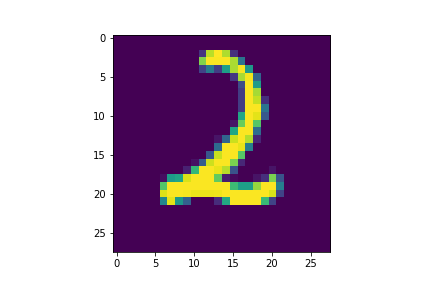
\includegraphics[width=0.4\textwidth]{two.png}
    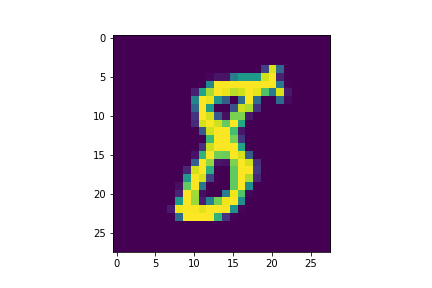
\includegraphics[width=0.4\textwidth]{eight.png}
  \end{center}
  \caption{Two numerals, handwritten by humans; they are part of the MNIST dataset.}
  \label{fig-mnist}
\end{figure}

\begin{figure}
  \begin{center}
   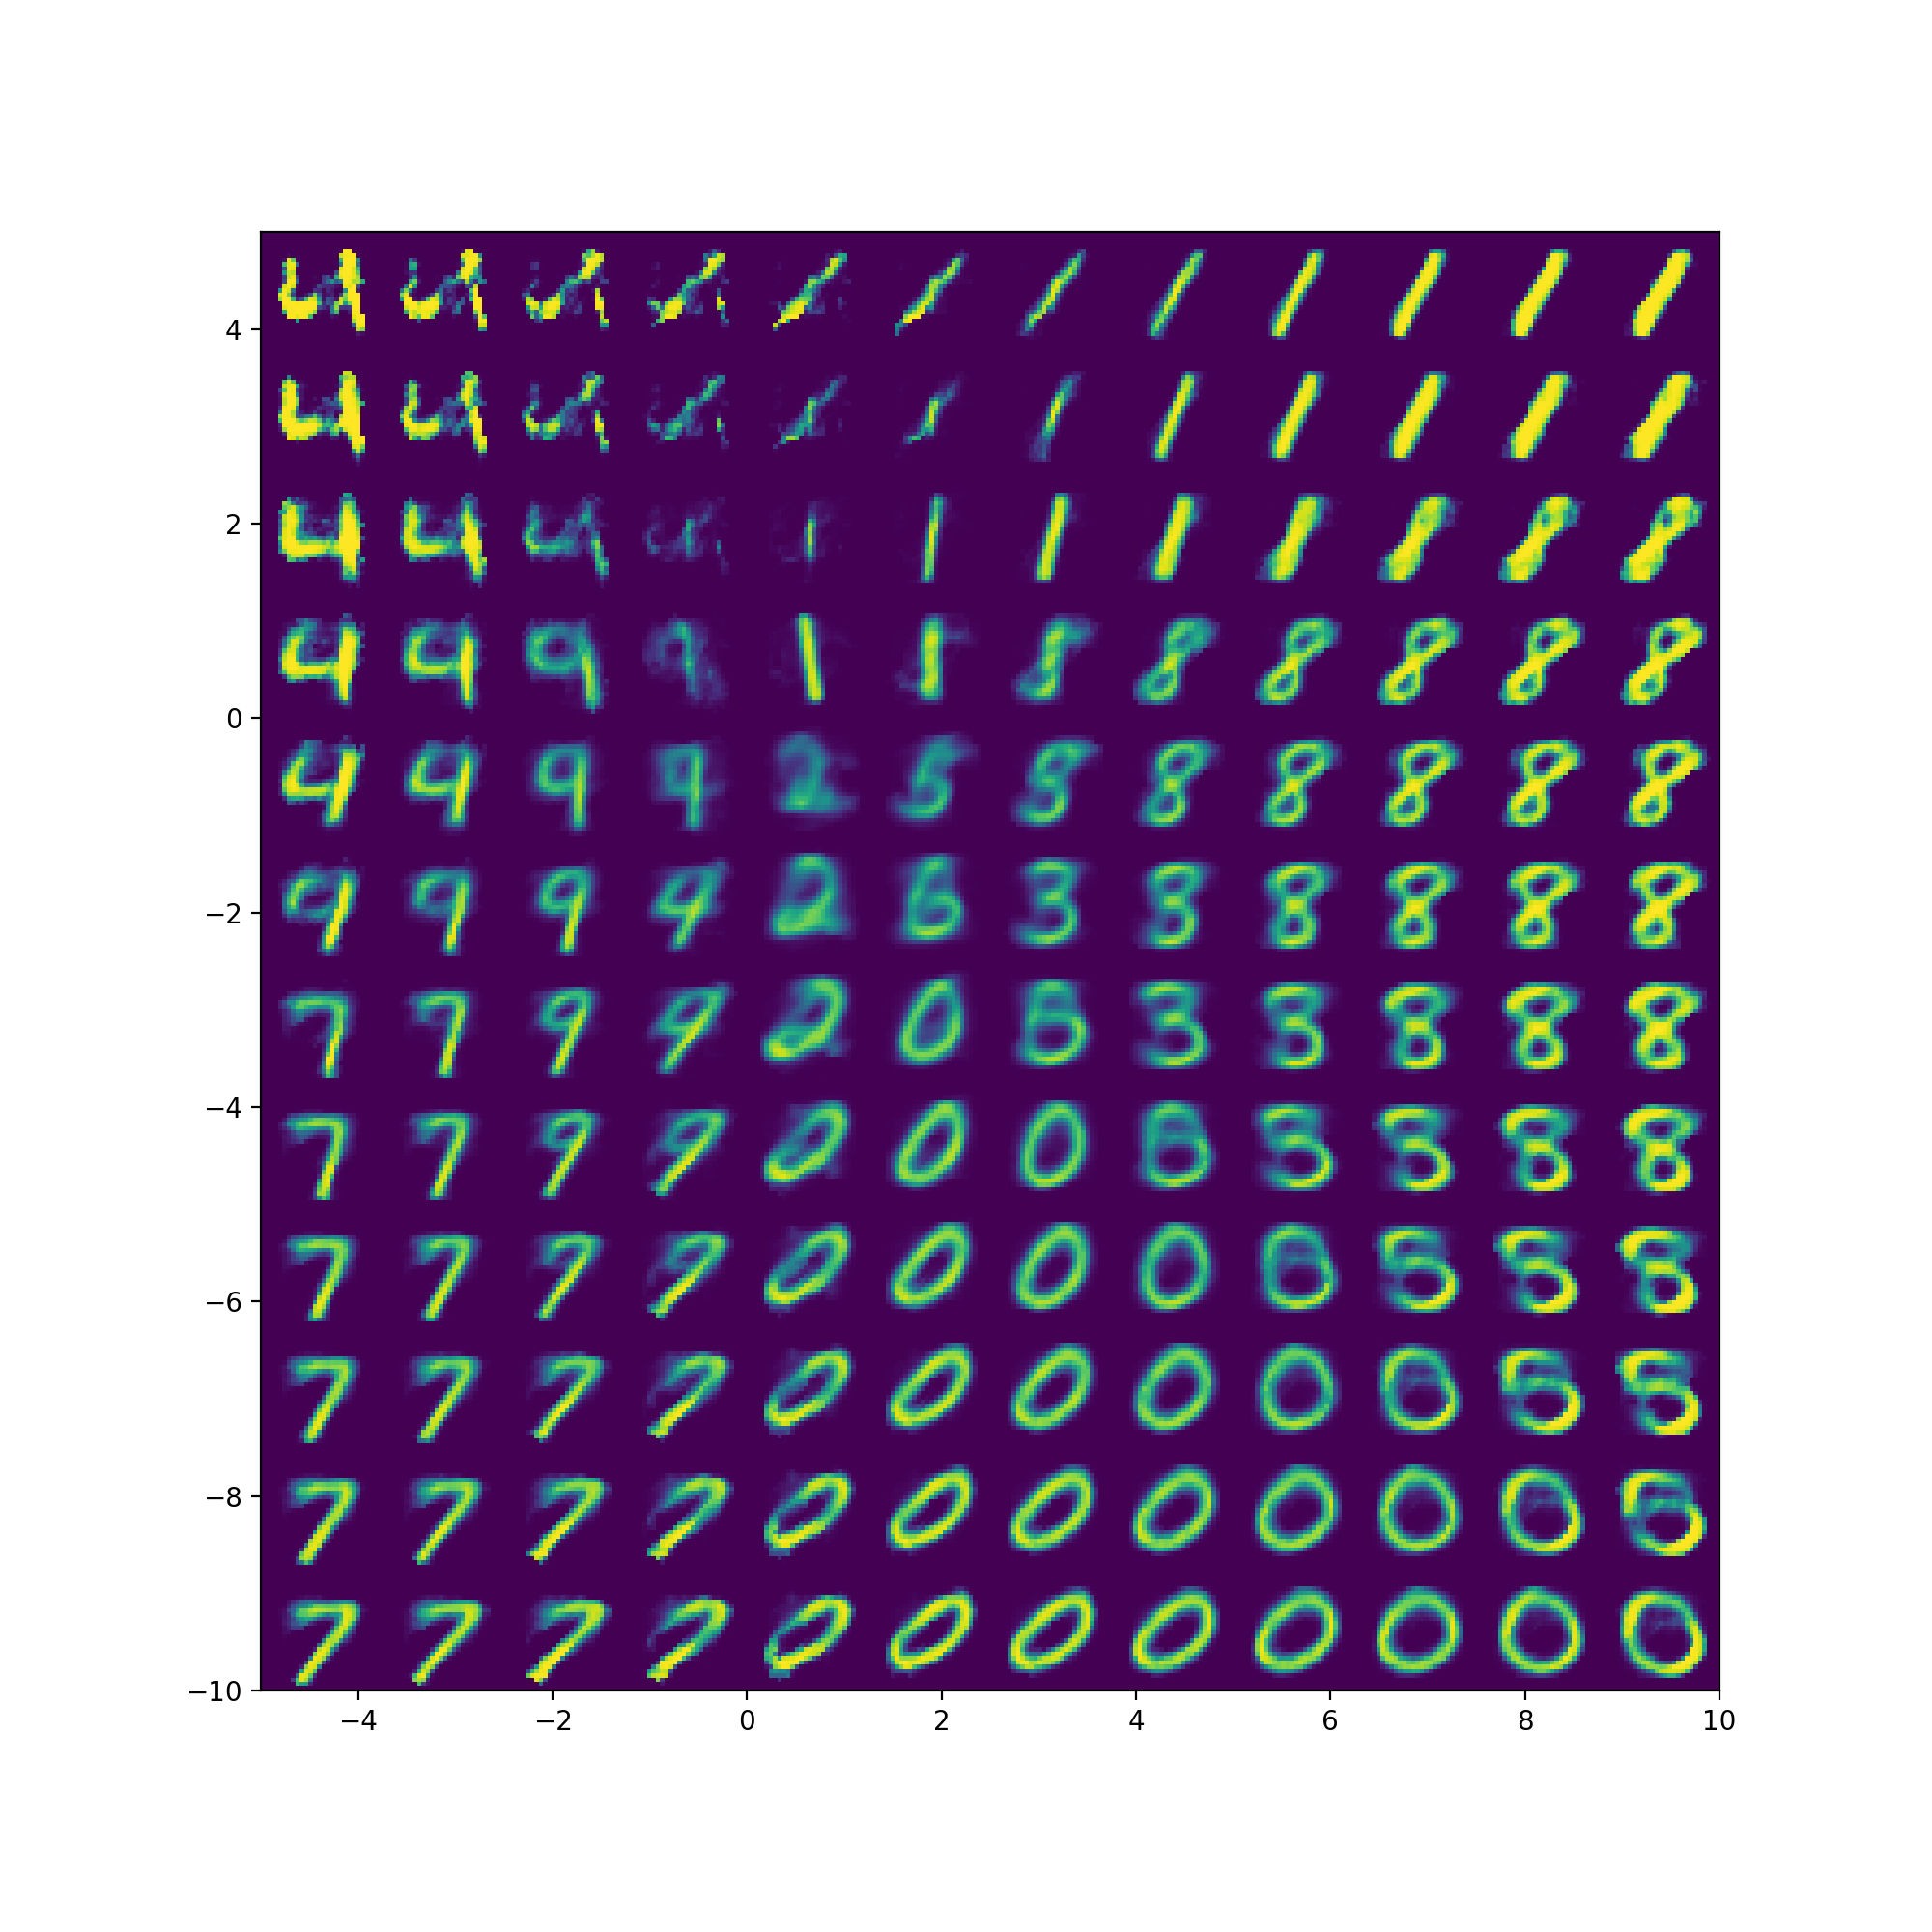
\includegraphics[width=0.7\textwidth]{synthetic.png}
  \end{center}
  \caption{Images that have been sampled from
  a generative model of human handwriting.}
  \label{fig-synthetic}
\end{figure}


Yet, the construction of generative models is arguably one of the major developments of the last decade in artificial intelligence. You will have seen examples of
synthetically generated faces that look like interpolations of real people. A simpler example is shown in Fig. \ref{fig-mnist} where a number of handwritten
numerals are shown together with one that has been synthetically generated (Fig \ref{fig-synthetic}).

The image generation process, to which we will return in Unit 5 and 6, considers the space of all possible pixel values. The images shown consist of $28 \times 28$
pixels. For simplicity, assume that pixels are black or white (in the actual dataset they are grey-scale values, but this does not really affect the argument). The space of
all possible images, $\mathcal{I}$, where each separate image is a different point, has dimension $2^{784}$. In generative modelling, it is assumed that an unknown
probability distribution $p(\boldsymbol{x})$ exists over the space $\mathcal{I}$. This probability distribution assigns a small positive probability
to each image that can plausibly
represent a handwritten numeral, and probability zero to images that do not. Next, a number of humans actually produce handwritten numerals, that are digitised
and brought into the $28 \times 28$ format. These images are collected in the so-called MNIST dataset \url{http://yann.lecun.com/exdb/mnist/},
an important dataset for benchmarking machine learning algorithms.
These human-drawn images are then considered to be samples, drawn from distribution $p(\boldsymbol{x})$, which are then
used to used to learn an approximation to this function. There are many ways of doing this. One of them learns a mapping from images to a set of Gaussian distributions through
a so-called \emph{encoder} network. A user can then sample from this Gaussian and feed the sample into a \emph{decoder} network that converts the sample into an image.

We will later encounter examples how \emph{encoder-decoder} networks are trained, but this architecture is now a core element of artificial intelligence techniques. In some such
techniques, such as \emph{variational autoencoders} the generative model described above is still recognisably present. It is hard to overestimate its importance.




\section{Fixed Basis Functions}

\begin{figure}[!ht]
  \begin{center}
    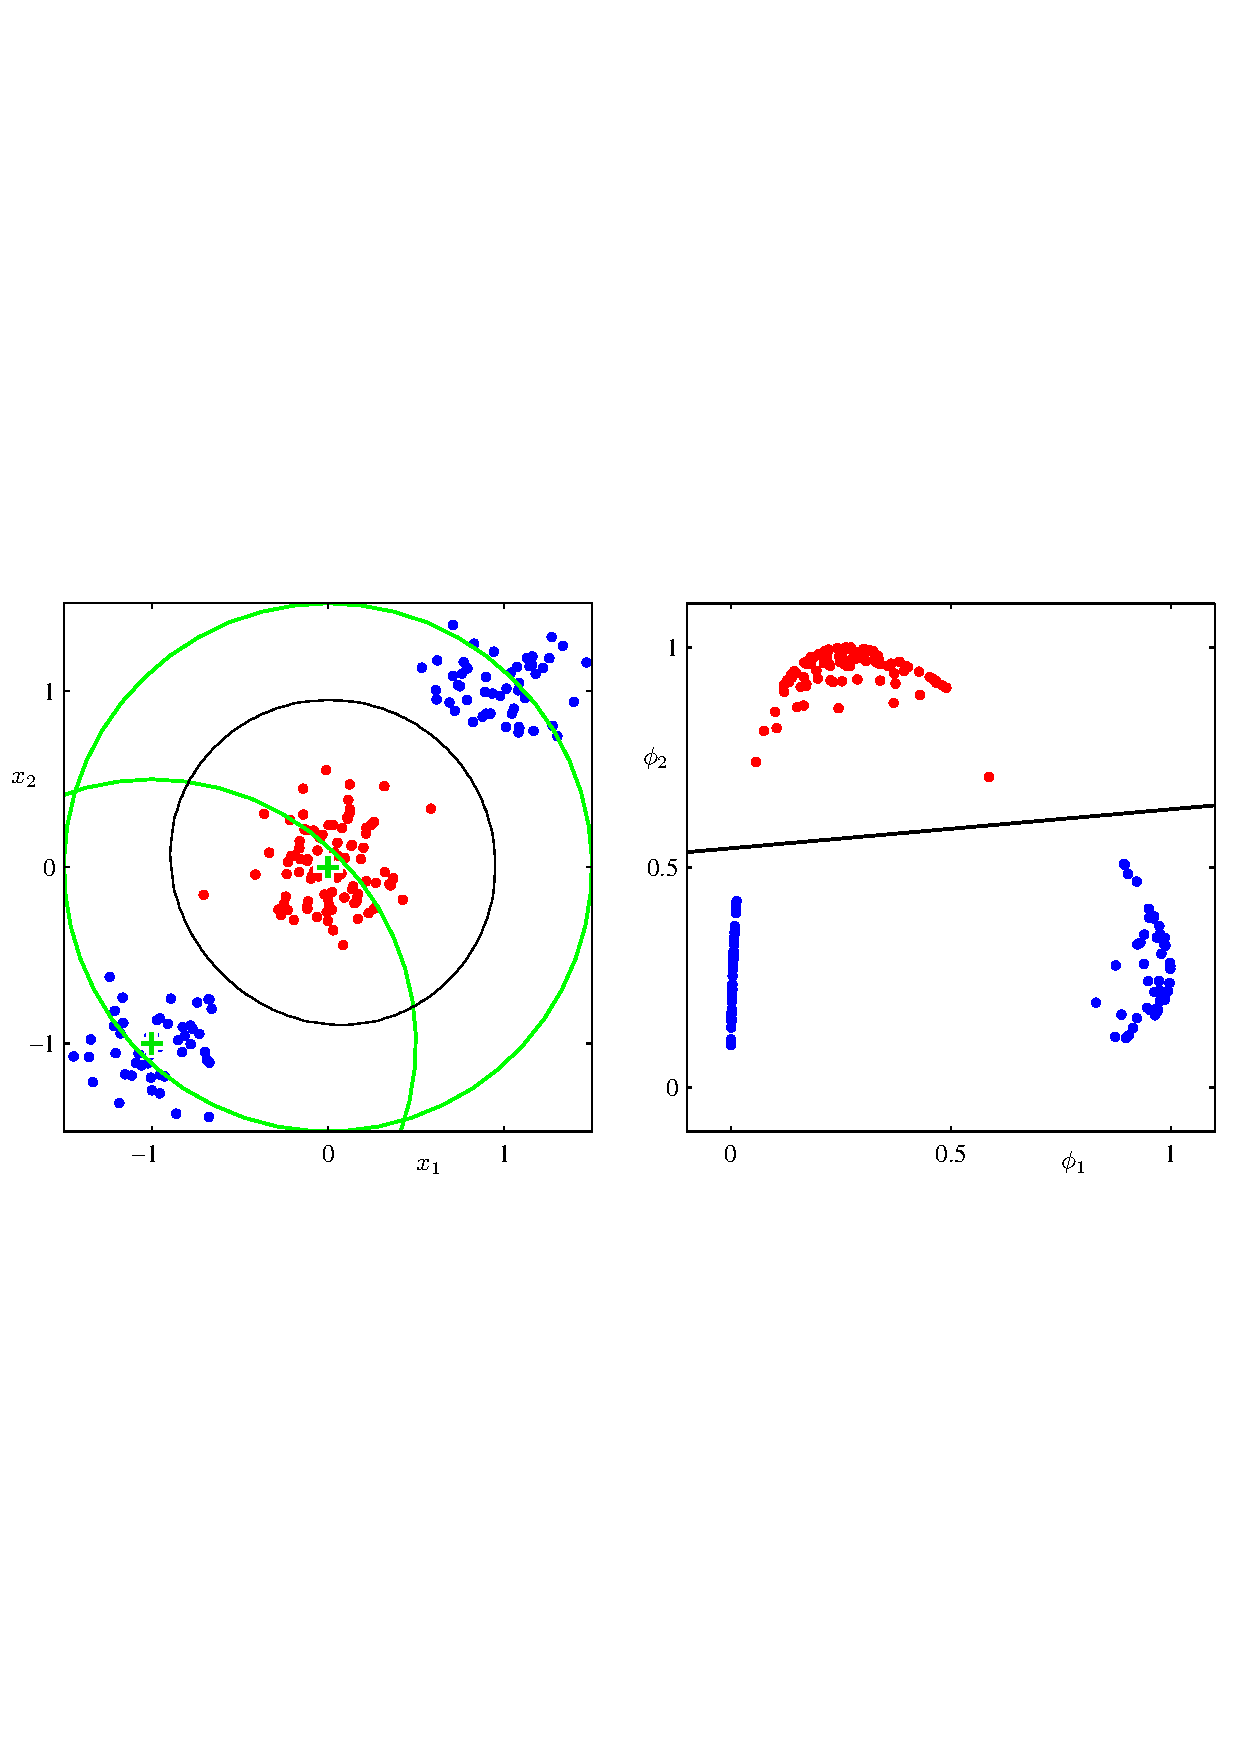
\includegraphics[width=0.9\textwidth]{Basisfunction.pdf}
  \end{center}
  \caption{A well chosen non linear transformation of the data can often reduce in a much simpler classification problem. Two 'Gaussian' basis functions
    are shown, their centres represented by green crosses, and contours by green circles in the left hand plot. The right hand plot shows the
    data in feature space $(\phi_1, \phi_2)$. Here the problem is linearly separable. This figure
  is Fig. 4.12 from Bishop (2006).}
   \label{fig-circular}
\end{figure}

Before starting with the formalism, it is useful to realise that just like in linear regression, discussed in Unit 1, we often do not regress on the data points
directly, but on fixed functions of the data points called \emph{basis functions}. The motivation is straightforward and illustrated in Fig. \ref{fig-circular}:
The original of dataset, shown in the left figure does not even  appear to be connected, but a simple transformation of the data renders it linearly separable,
as shown on the right.
For this reason, we develop the formalism on basis functions of the data points rather than the data points themselves. Mathematically, it is just as
complicated to work with fixed basic functions as directly with the data points as we shall see.

 How does one find these basis functions? Often they suggest themselves: the transformation in Fig. \ref{fig-circular} would be hard to miss and any data scientist
 should be on the lookout for opportunities to simplify their problem. But here, neural networks come into their own. They can be seen as methods that are capable
 of learning basis functions that are appropriate for a given dataset. We will give examples when we have developed the \emph{multi-layer perceptron} later.

\section{Multi-class Logistic Regression}
  \begin{figure}
    \begin{center}
      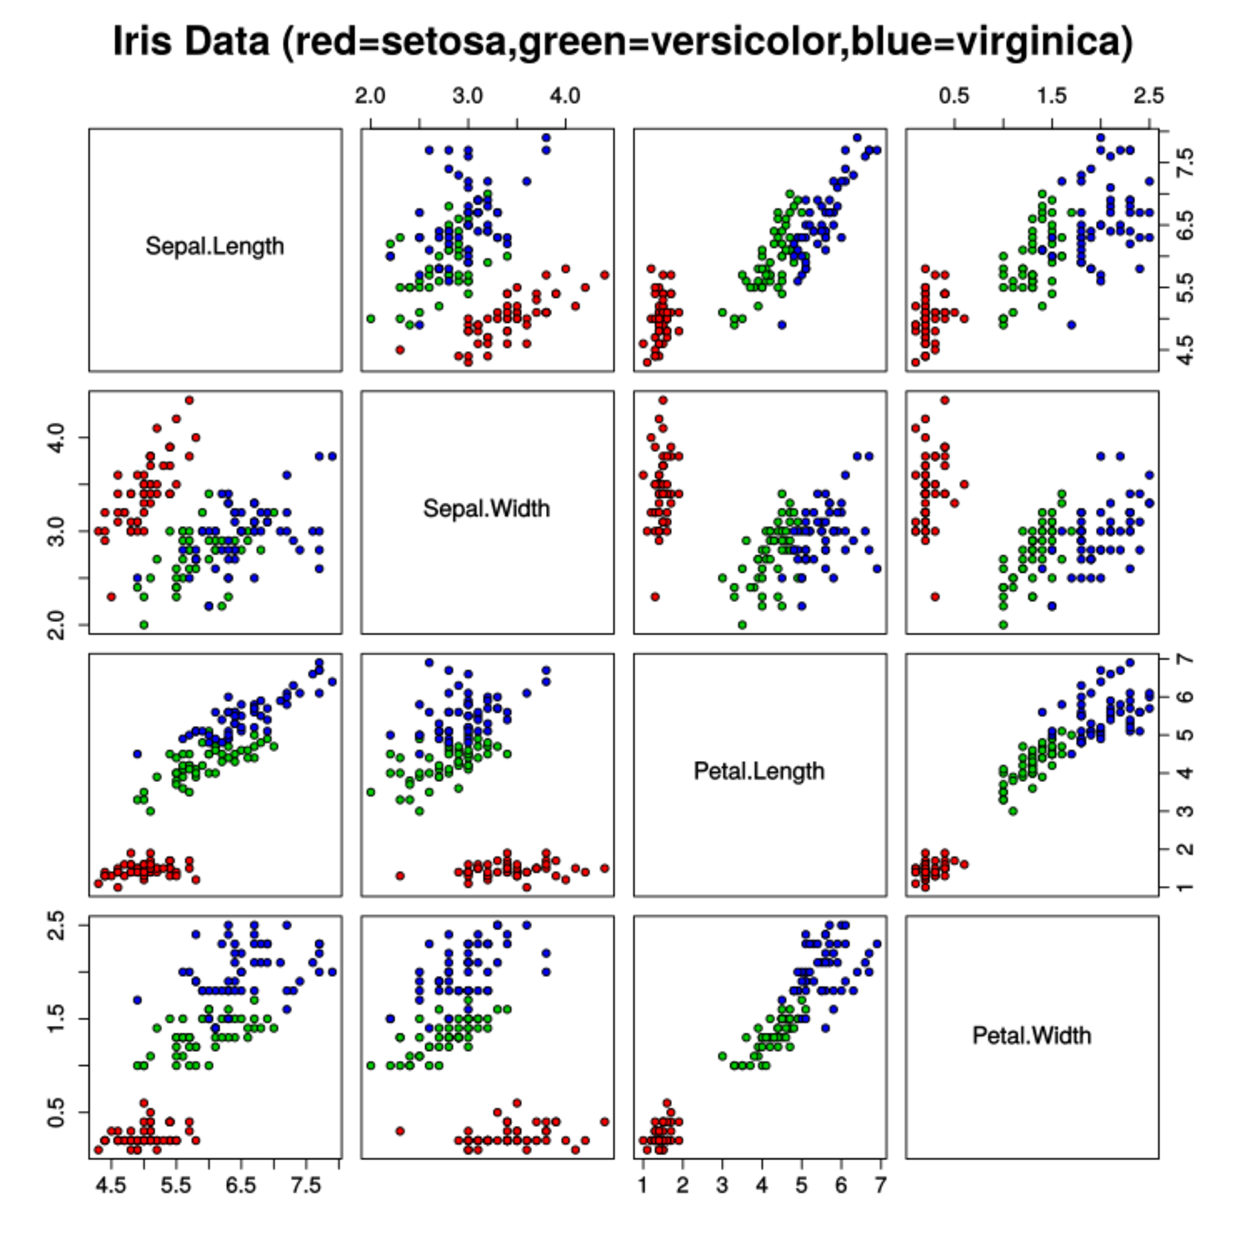
\includegraphics[width=0.7\textwidth]{Iris_dataset_scatterplot.pdf}
    \end{center}
    \caption{The Iris dataset represented, wastefully, as a set of scatter plots between the four dimensions of each flower.}
    \label{fig-iris}
  \end{figure}

\label{sec-multiclass}
  Often, we want to create classifiers that can handle more than one class. An example is the so-called iris dataset. It is possible to distinguish three varieties
  of irises, \emph{virginica}, \emph{setosa} and  \emph{versicolor} by measuring their sepal length, sepal width, petal length and petal width (SL, SW, PL, PW).
  The dataset is a well known toy problem in machine learning.
  It is shown in Fig. \ref{fig-iris}. Suppose we would want to build a classifier that accepts the four numbers (SL, SW, PL, PW) and predicts one of the three varieties
  \emph{setosa}, \emph{virginica}, \emph{versicolor} Source: Wikipedia.
  
  \begin{figure}[!ht]
    \begin{center}
      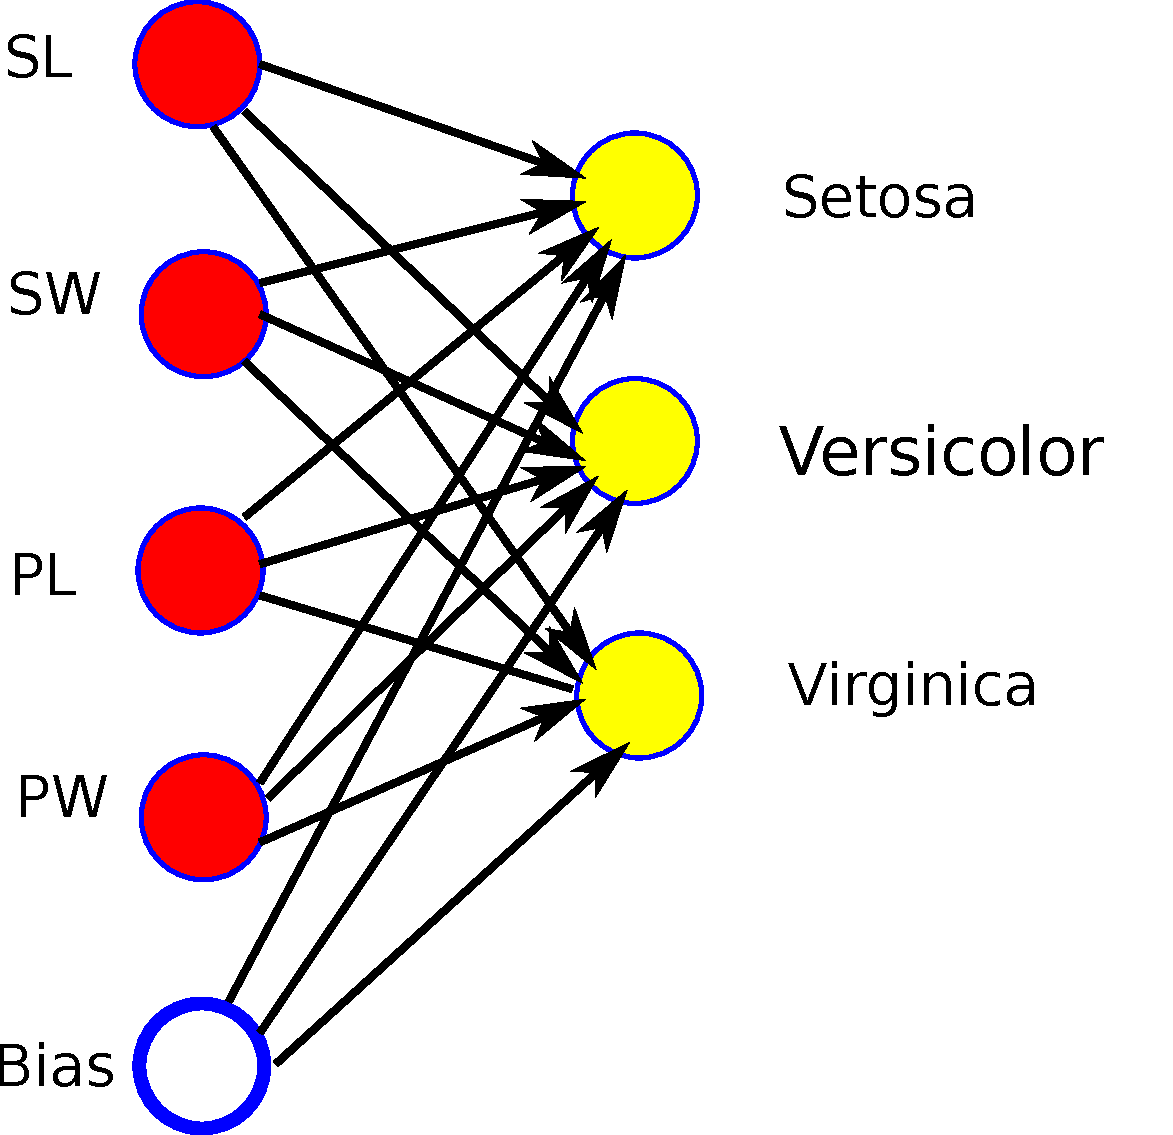
\includegraphics[width=0.7\textwidth]{irisnetperc.pdf}
    \end{center}
    \caption{A two-layer neural network built from three perceptrons, run in parallel. It has four input nodes: \emph{petal length}, \emph{petal width}, \emph{sepal length},
      \emph{sepal width} and a single bias node, whose value is always 1. Each perceptron takes a yes/no decision about one of the three classes: setosa,
      versicolor and virginica. If each of the perceptrons were perfect, a one hot encoding would emerge were the activation of a single node would indicate which
      iris variety the input dimensions belong to. The perceptron trying to recognise versicolor will not work well.}
    \label{eq-irisnetperc}
  \end{figure}




 The iris dataset can serve as a model here: any iris in the dataset belongs to one and only
 one class, but there are three classes. In multi-class logistic regression the goal is  for a given data point to find the probability that it belongs
 to class $\mathcal{C}_1$, $\mathcal{C}_2$ and $\mathcal{C}_3$. This gives three probability
values which must sum to 1. For the $K$-class case, one finds, taking into account the possible use of basis functions:

\begin{equation}
  p(\mathcal{C}_k \mid \boldsymbol{\phi}) = y_k(\phi) = \frac{\exp a_k}{\sum_j \exp a_j},
  \label{eq-softmax}
\end{equation}
with
$$
a_k = \boldsymbol{w}^T_k \phi.
$$

Eq. \ref{eq-softmax} is called a \emph{soft-max function}. It is not hard to verify that the $0 < y_k < 1$ and $\sum_k y_k = 1$, so they have a natural
interpretation as probabilities. Overflows can sometimes occur in numerical evaluations of Eq. \ref{eq-softmax} as the exponentials may evaluate to large
numbers. This problem is easy to avoid if you are aware of it. The notebook \emph{Logistic Regression on MNIST} gives an example of a safe implementation.

\begin{figure}[!ht]
  \begin{center}
    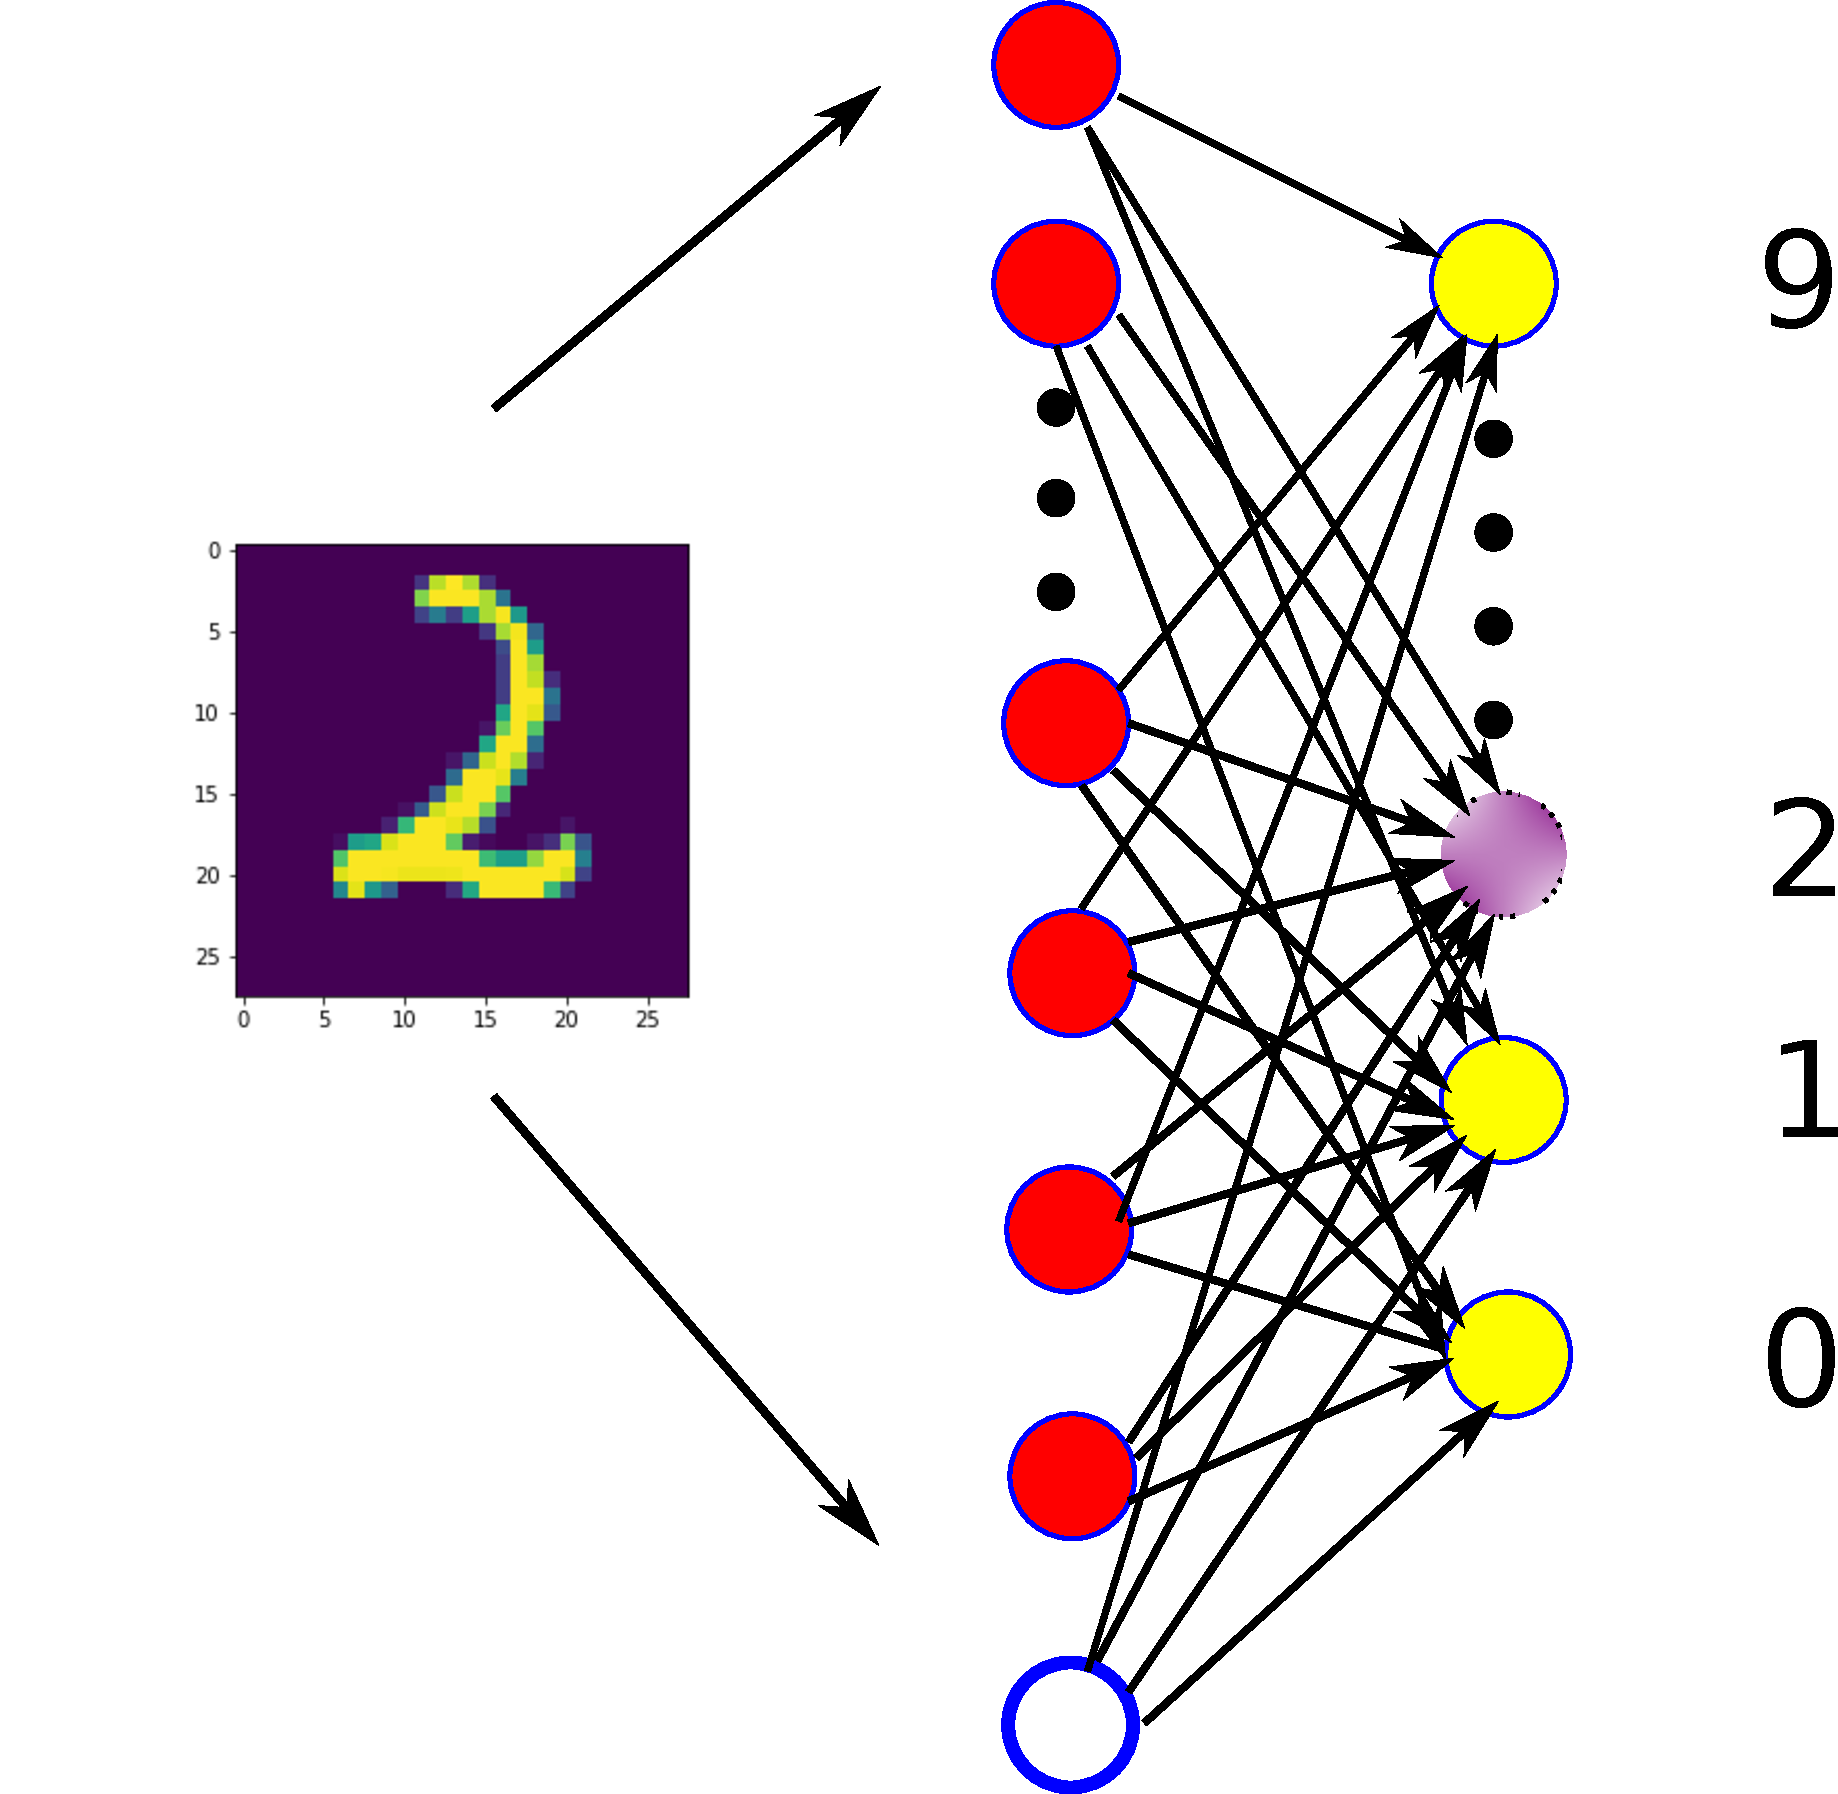
\includegraphics[width=0.7\textwidth]{mnist.pdf}
  \end{center}
  \caption{An example of multi-class logistic regression. There are 785 input variables: $28 \times 28 = 784$ pixels and a bias node. There are
    ten classes. The desired output is a 1-over-10 ('one hot') representation of the number that the regressor believes the image represents.
    For the regressor the spatial representation of the image does not play a role. The input image is 'flattened' to a vector.}
  \label{fig-logmnist}
\end{figure}

  


In classification problems, a one-hot encoding, also called one-over-k encoding is natural for labelled data. For example, for the iris data set
\emph{setosa}, \emph{virginica} and \emph{versicolor} may be represented as $(1, 0, 0), (0, 1, 0)$ and $(0, 0, 1)$, which may be compared to softmax outputs as these
to can be interpreted as a set of probabilities. Another example is the MNIST dataset, where a one-over-10 encoding is used to provide labels for image classification.
The regressor is trained to infer the numerical value that is represented by the image using the labels provided as part of the dataset.
As Fig. \ref{fig-logmnist} shows, the regressor may be interpreted as a two-layer neural network.



Since the softmax outputs are meant to represent probabilities and add to one, in the derivation of the gradient there is a subtlety
in that the output values are not independent. In order
to find the gradient, one needs the derivative of the output values with respect to the activation values. This is given by:
\begin{equation}
  \frac{\partial y_k}{\partial a_j} = y_k(\delta_{kj} - y_j),
\end{equation}
where $\delta_{kj}$ are the components of the identity matrix.

Also, the likelihood function requires adaption. We adopt the 1-of-$K$ coding scheme. For $K$ nodes there
will be one that is active '1', whilst the others are silent '0'. So the target vector $t_i$ for a feature vector $\boldsymbol{\phi}_i$
belonging to class $\mathcal{C}_k$ is a binary vector with all elements zero, except for element $k$, which equals one.

The likelihood function is then given by:
$$
p(\boldsymbol{T} \mid \boldsymbol{w}_1, \cdots, \boldsymbol{w}_k) = \Pi^K_{k=1}\Pi^N_{i=1} p(C_k \mid \boldsymbol{\phi}_i^{t_{ik}}) = \Pi^K_{k=1}\Pi^N_{i=1} y^{t_{ik}}_{ik}. 
$$
  
Here $y_{ik} = y_k(\boldsymbol{\phi}_i)$ and $\boldsymbol{T}$ is an $N \times K$ matrix of target variables with components $t_{ik}$.
The negative log likelihood is given by:
$$
E(\boldsymbol{w}_1, \cdots \boldsymbol{w}_K) = - \ln p(\boldsymbol{T} \mid \boldsymbol{w}_1, \cdots \boldsymbol{w}_K) = -\sum^K_{k=1}\sum^N_{i=1} t_{ik} \ln y_{ik}.
$$
The gradient follows from a calculation that is similar to the two-class case:
$$
\frac{\partial E}{\partial \boldsymbol{w}_j} = \sum^N_{i=1}( y_{ij} - t_{ij}) \boldsymbol{\phi}_i.
$$




Having calculated the gradient, we can apply \emph{stochastic gradient descent} as earlier. We give an example in the notebook \emph{Logistic Regression on MNIST},
where we build a classifier that can recognise the number represented by a handwritten image with reasonable (87 \%) accuracy. In the notebook,
you can look at images that are wrongly classified, which is instructive.


The second order methods work, in principle, but if the number
of classes increases, straightforward IRLS becomes impossible as the memory demands scale as $D(C-1) \times D(C-1)$, where $D$ is the number of data points and
$C$ the number of classes. The matrices for a 10-class logistic regression problem are 25 times as large as for a 2-class problem. Section 8.3.7 of \cite{murphy2012}
discusses this problem and mitigating strategies.


In \emph{Activity MNIST Logistic Regression} you will investigate whether the iris dataset can be classified using logistic regression.

\subsection{A Comment on the Choice of Loss Functions.}
Throughout logistic regression, we have used the cross entropy as a loss function. Could we have used the MSE function? Yes, but this is treating classification
as regression. Although the one-over-$K$ vectors can be used as a target for regression, these values have no probabilistic interpretation. They are just numbers.
In the soft-max output and the cross-entropy loss function, the probabilistic interpretation is baked in. Moreover, we have seen in Unit 1 that predicting
outputs that are unlikely to have been generated by the true distribution lead to very high costs. For classification the cross entropy is the better choice of
loss function.


\chapter{Na\"ive Bayes}
\section{Introduction}
Na\"ive Bayes is a way of building fast and cheap classifiers by making an assumption about the data generation mechanism that is completely unrealistic in general, but that
often achieves decent classification results. Historically, an important application has been spam filters: adaptive classifiers that are able to pick up spam messages if
particular messages are flagged often enough as spam by a human. They can be trained online, meaning they can continue to train on novel messages.
The na\"ive Bayes assumption states that events are independent conditional on the class that belong to. This statement probably needs unpacking. We already have encountered
one example of the na\"ive Bayes assumption: the iris dataset. Consider, again Fig. \ref{fig-iris}: we see that there are three classes corresponding to the three iris
varieties and that a data point comprises four features and a classification. The na\"ive Bayes assumption states that the probabilities for generating these data points
are independent conditional on class. Mathematically, this means that:
\begin{equation}
  p(\vec{x}_1, \vec{x}_2, \cdots, \vec{x}_{N_i} \mid \mathcal{C}_i) = p(\vec{x}_1 \mid \mathcal{C}_i) p( \vec{x}_2 \mid \mathcal{C}_i) \cdots p(\vec{x}_{N_i} \mid \mathcal{C}_i ).
  \label{eq-nb}
\end{equation}
Here $\vec{x}_i$ is a four-dimensional vector $(P_L, P_W, S_L, S_W)$ and $\mathcal{C}_i$ is one of the the three classes that the flower represented by data point $i$
belongs to. So there are three classes: $\mathcal{C}_1 = \mbox{virginica}$ etc. Eq. \ref{eq-nb} hides a number of assumptions about the data generation mechanism.
First, we assume that we can find probability density functions that are valid for each class individually, meaning that we assume that we can find independent data
generation mechanisms for  each iris variety. This is not unreasonable: there is probably a lot that the different varieties have in common, but there must be some biological
factor that controls which variety the flower will belong to. A second, much stronger assumption is represented by Eq. \ref{eq-nb}: the in-class probabilities for generating
flower dimensions are independent and described by the same distribution $p(\vec{x}_i \mid \mathcal{C}_i)$. This is a strong assumption: it states that the data generation
for each data point is independent of another data point once the class is determined and that you can sample a single distribution for a given iris variety to obtain data
points that are representative for that variety. In more technical language: every pair of features is conditionally independent given class membership.

The distributions of the three coloured markers are blobs that are somewhat reminiscent of Gaussian distributions. Thus inspired, we might guess that:
$$
p(x_i \mid \mathcal{C}_i) = \mathcal{N}(\mu_i, \Sigma_i),
$$
that is: each of the blob is described by a Gaussian distribution with a different mean and covariance for each of the three classes. Now we can use Bayes' law:
\begin{align}
  p(\mathcal{C}_i \mid \vec{x}_1, \vec{x}_2, \cdots \vec{X}_N) \mid \mathcal{C}_i) & \sim  p(\vec{x}_1, \vec{x}_2, \cdots \vec{x}_N \mid \mathcal{C}_i )  p(\mathcal{C}_i) \\ \nonumber
   & \sim \Pi^N_{i=1} \mathcal{N}( \vec{x}_i \mid \mathcal{C}_i) p(\mathcal{C}_i)
\end{align}
In particular, this is true for a single data point $\vec{x}$:
$$
p(\mathcal{C}_i \mid \vec{x}) \sim p( \vec{x} | C_i )p(\mathcal{C}_i)
$$

This now opens the way for a very simple classification procedure:
\begin{enumerate}
  \item For each class estimate the prior probabilities $p_{virginica}$, $p_{setosa}$, $p_{versicolor}$, simply by counting the number of entries for each of the varieties
  and dividing by the number of total entries. For the iris dataset there are 50 data points of each class so these prior probabilities are equal to $\frac{1}{3}$.

\item For each of the varieties estimate the means and the covariance matrices. The standard estimators introduced in unit 1 will do, but \emph{scikit-learn} or \emph{scipy}
  offer functions to do this.

\item With these estimates you calculate $\mathcal{N}(\vec{x} \mu_{virginica}, \Sigma_{virginica})p_{virginica}$, $\mathcal{N}(\vec{x} \mu_{setosa}, \Sigma_{setosa})p_{setosa}$, and $\mathcal{N}(\vec{x} \mu_{versicolor}, \Sigma_{versicolor})p_{versicolor}$.

\item Whichever of these three is largest determines which class $\vec{x}$ should belong to.   
\end{enumerate}

The resulting classifier is quite good. We show the result of a notebook \emph{A Na\"ive Bayes Classifier for the Iris Dataset} in Fig. \ref{fig-naiveiris}. Exploration
of this notebook will demonstrate the workings of a na\"ive Bayes classifier for this dataset.

\begin{figure}
  \begin{center}
    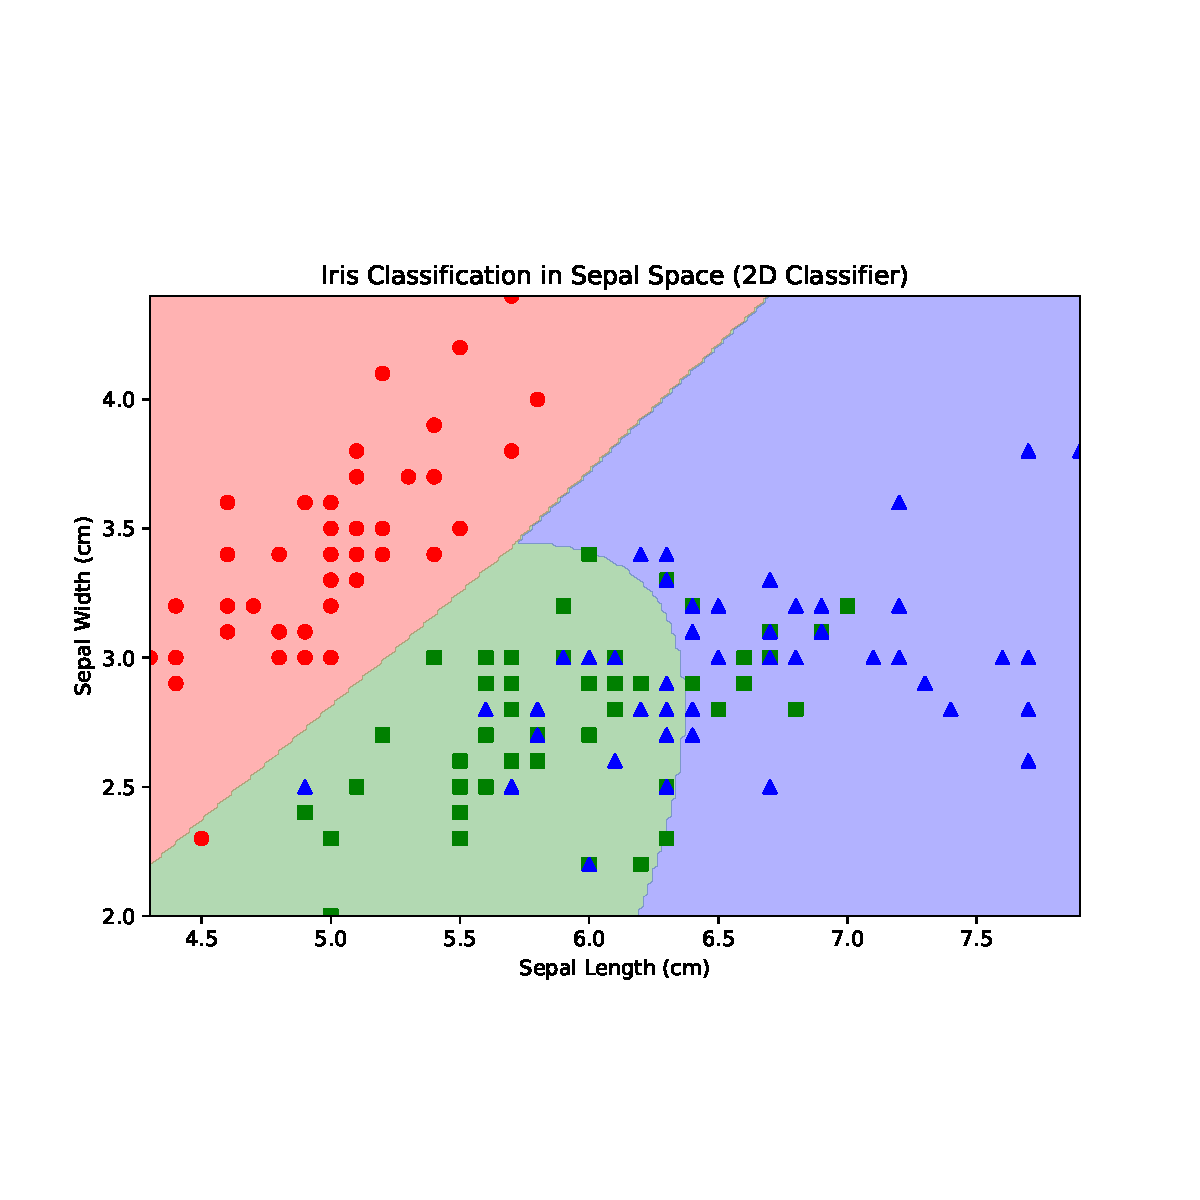
\includegraphics[width=0.8\textwidth]{naiveiris.pdf}
    \caption{A 2D scatter plot of the sepal length/sepal width feature of the iris dataset. The markers indicate different iris varieties. A 2D na\"ive Bayes classifier
      shows the different classification volumes and shows decent performance. The 4D version, which uses all four features performs even better but does not have
      a simple visualisation.}
    \label{fig-naiveiris}
    \end{center}
  
\end{figure}

\subsection{Na\"ive Bayes and Logistic Regression}
The na\"ive Byes classifier described in the previous section is equivalent to the generative interpretation of logistic regression. Imagine that we would not be faced
with a three-class classification problem as in the case of the iris dataset, but with a two-class problem. Then we would have exactly the method described in Sec.
\ref{sec-generative}. There too, we assumed a generative model defined by two Gaussian distributions, one for the 'red' class of points and one for the 'blue' class of points,
and we proved mathematically that this leads to a logistic regressor.

For the three-class classification it is more work, but here too you can show that it leads to a logistic classifier. Please be aware of the distinction between the
na\"ive Bayes assumption and the generative model itself. The generative model is just an algorithm for constructing a dataset. The na\"ive Bayes assumption is an assumption about real data, in this case that the iris dataset can be reasonably described by a generative model that is class dependent but that has independent probabilities for
data generation within any class.

\subsection{A Spam Filter}
The na\"ive Bayes assumption does not look completely ridiculous. Here, we will show an application where it is highly questionable, but nonetheless leads to a
good classifier.
Let's consider the case of whether we want to establish whether an email is genuine ('ham') or spam ('spam'). This means that we two classes $\mathcal{C}_{spam}$ and $\mathcal{C}_{ham}$. Now consider a very simple vocabulary:
[ 'profit','sex', 'curtain', 'phone', 'notebook', 'hair extension', 'vindaloo']. This is now a word list:
$w_i, i = 0, \cdots, 6$. E.g. $w_2$ = \emph{curtain}.



According to the \emph{bag of word} model, every message can be written as a binary feature vector. Simply look at a message, determine if the $w_i$ is present. If it is, set a variable $b_i =1$, otherwise $b_i = 0$. Do this for all words in your vocabulary and your message will be transformed in a binary feature vector $\vec{b}$. So the text message: "Your notebook is part of your hair extension" would translate into the vector $\vec{b} = (0, 0, 0, 0, 1, 1, 0)^T$. Importantly, the order in which the elements of the vector are kept doesn't matter. There is no attempt to preserve the original word order from the message.

Imagine that we have a dataset of text messages that we now can represent as a collection of such vectors. So we can 5 'ham' messages and 4 'spam' messages.
$$
B_{ham} = \begin{pmatrix} 1 & 0 & 0 & 1 & 0 & 1 & 0 \\
                          0 & 1 & 1 & 1 & 0 & 0 & 1 \\
                          0 & 0 & 1 & 1 & 1 & 0 & 1 \\
                          1 & 0 & 0 & 1 & 0 & 1 & 0 \\
                          0 & 0 & 1 & 0 & 0 & 0 & 0 \\
                          1 & 0 & 1 & 1 & 0 & 0 & 1
                          \end{pmatrix}
$$
The spam messages are represented by:
$$
B_{spam} = \begin{pmatrix} 1 & 1 & 1 & 0 & 1 & 0 & 0\\
                           0 & 1 & 0 & 0 & 1 & 1 & 0 \\
                           0 & 0 & 1 & 1 & 0 & 1 & 1\\
                           1 & 1 & 1 & 0 & 1 & 0 & 0
                           \end{pmatrix}
$$
Your very welcome to speculate on the actual text content. This is not necessarily a realistic example, but it serves to identify the main probabilities that play a role.

A reasonable estimate is:
$$
p_{ham} = \frac{6}{10}
$$
and
$$
p_{spam} = \frac{4}{10}
$$

It is equally easy to estimate the probabilities $P(w_i \mid \mathcal{C}_j)$. As an example, look at
$P(w_1 | 'ham') = \frac{3}{6}$. Why? Add the number of ones in the first column of $B_{ham}$. We see that word 1
occurred three times out of a total of 6. You should be able to verify easily that:


\begin{table}
  \begin{center}
  \begin{tabular}{|r|r|r|} \hline
 Word & Ham & Spam  \\ \hline
 1    & 3/6 & 2/4  \\
 2    & 1/6 & 3/4  \\
 3    & 4/6 & 3/4  \\
 4    & 5/6 & 1/4  \\
 5    & 1/6 & 3/4  \\
 6    & 2/6 & 2/4  \\
 7    & 3/6 & 1/4  \\ \hline
  \end{tabular}
  \end{center}
  \caption{The probabilities $P(w_i \mid C_j)$ for $i= 1, \cdots, 7$, $j = \mbox{ham}, \mbox{spam}$, estimated from the feature representations of the set of messages.}
  \label{tab-wc}
\end{table}
We now consider the following generative model: for each word in the vocabulary, the probability of the word being absent ($b_i = 0$) or present ($b_i = 1$) is determined by a Bernoulli process. The generative process works as follows:

\begin{enumerate}
\item Decide whether a message is 'ham' or 'spam'. This is a Bernoulli process where the probability of $x = 1$, i.e.
the message is 'spam' is given by $P('ham')$.
\item The class $\mathcal{C}_i$ is now given as the outcome of the sampling process: $i = 0$: 'ham'; $i = 1$: 'spam'. The probability for generating a single word is again given by the Bernoulli process, and the *bag of words* assumption states that these probabilities should be independent, meaning that we can write down the
probability of generating a feature vector given the class as:
\end{enumerate}
$$
p(\boldsymbol{b}| \mathcal{C}_j ) = \Pi^N_{i=1} p(w_i | \mathcal{C}_j )^b_i ( 1 - p( w_i | \mathcal{C}_j)^{1 - b_i}
$$
Here $N$ is the number of words in the vocabulary and $i$ labels the words in there.

\section{The Na\"ive Bayes Assumption}
The \emph{Na\"ive Bayes} assumption is strongly related to the bag of words model, but Naive Bayes is an assumption about how real messages are generated. The assumption is that also in real emails the features are independent when conditioned on class. How does that help?

What we're really interested in is:
$$
p(C_i \mid \boldsymbol{b}),
$$

Now $\boldsymbol{b}$ actually stands for a real e-mail, reduced to its features.

or rather we are interested in whether
$$
p(C_1 \mid \boldsymbol{b}) > p(C_0 \mid \boldsymbol{b})
$$ 
because if that's the case we classify the message as 'spam', and if it's not we label it as 'ham'.

By now your instinct should be to invoke Bayes' law:
$$
p(C_i \mid \boldsymbol{b} ) \sim p(\boldsymbol{b} \mid C_i) p(C_i)
$$
This ignores the normalisation constant, something we will deal with below. It is now important to realise that $\vec{b}$ is the feature vector of a real e-mail message, s
o $p(\boldsymbol{b} \mid C_i)$ is the probability of an actual e-mail message occurring. It is difficult to estimate the probability in practice: an e-mail may be unique.

The \emph{na\"ive Bayes assumption} is that features are independent given the class, i.e. conditionally independent. This should immediately raise suspicions.
It states that if we know that a message is 'ham', the probabilities for each of the vocabulary words occurring are independent of each other. This is patently untrue in the
case of natural language, which is why this assumption is na\"ive. Take a moment to find counterexamples that demonstrate this. For classification purposes, nonetheless, t
his is ignored and the assumption is made anyway. It turns out that for classification purposes this often works reasonably well.

The naive Bayes assumption here states that:
$$
P(\boldsymbol{b} \mid C_j) = \Pi^N_{i=1} P(b_i \mid C_j) = \Pi^N_{i=1} P(w_i \mid C_j)^{b_i}(1 - P(w_i \mid C_j)^{1 - b_i} 
$$
Now the probability for finding a certain message, which we cannot reasonably be expected to estimate, has been replaced by products of probabilities that certain words are
occurring, which we can estimate.

Note that the formulae we arrived at are the same as for the generative model, but that the ideas are different. In the generative model, we made a \emph{bag of word}
assumption, deliberately generating documents that do not really look like real messages. They are really only realistic in that the word frequencies in ham or
spam messages are about right. In a generative model, we are free to make such assumption.

The naive Bayes assumption is an assumption about real natural language in real email messages. This assumption is wrong and only defensible on the basis that it seems to do
a reasonable job in classification. It is important to realise that both ideas lead to the same formulae but are fundamentally different.


\subsection{The Bayesian Two-class Classification  Problem}

As you will have seen in the notebooks of Unit 1, the determination of posterior probabilities using Bayes' Law requires the determination of a
normalisation constant, which can be tricky in practice. In a two-class classification problem
we can bypass this problem, because we're only interested in which of the two posterior probabilities is the larger one and we do not really care about their numerical value.
We will show this in detail here.

In spam classification we are interested in the function $p(C_i \mid w_1, w_2 \cdots w_N)$ (what is the the probability that this is spam given this set of features?). Bayes
then tells us that:
$$
p(C_1 \mid w_1, w_2 \cdots w_N) =  \frac{p(w_1, w_2 \cdots, w_N \mid C_1)}{p(w_1, w_2, \cdots w_N)} p(C_1)
$$
and similarly:
$$
p(C_2 \mid w_1, w_2 \cdots w_N) =  \frac{p(w_1, w_2 \cdots, w_N \mid C_2)}{p(w_1, w_2, \cdots w_N)} p(C_2)
$$

Now observe something that is generally true in two-class classification problems: the normalisation factor is identical in both cases.  We can make a decision, 'spam' or
'ham', based on whether the posterior probability is larger for ham or for spam. In other words, we can base that decision on which of the two is the larger one and we
can get infer that from dividing both equations and observe whether this ratio is larger or smaller than one:
$$
\frac{p('spam' \mid w_1, w_2, \cdots, w_N)}{p('ham' \mid w_1, w_2, \cdots, w_N)} =
\frac{p(w_1, w_2 \cdots, w_N \mid 'ham')p(('ham')}{p(w_1, w_2 \cdots, w_N \mid 'spam')p(('spam')}
$$
The overall normalisation constant drops out and can be ignored.  If this ratio is larger than 1, we decide 'spam', otherwise we decide 'ham'.
This idea applies generally to any Bayesian analysis of a two-class classification problem and is not restricted to naive Bayes scenarios.
\section{Putting it All Together}
When we put everything together we find that once we have estimated the prior probabilities $p_{'ham'}$ and
the probabilities $p_{'spam'}$, which we simply do by counting the number of spam and ham messages and dividing by the total, and once we have estimated the probabilities $p(w_i \mid \mathcal{C}_j)$, the classifier is trained. An interesting question is how to define the vocabulary. This can require some experimentation. The simplest solution is to build the vocabulary out of every word encountered in all messages. This is what we did
in the notebook \emph{Na\"ive Bayes - The Bernoulli Document Model}, where we apply this to a set
of SMS messages which have been classified 'ham or 'spam' (link is in the notebook). This works well
enough but could be refined. For example, the word
'the' is probably not very informative and might be left out.

Once the vocabulary has been defined, the messages can be reduced to feature vectors and
for every message you find whether
\begin{align}
\Pi^N_{i=1} P(w_i \mid C_{'spam'})^{b_i}(1 - P(w_i \mid C_{'spam'})^{1 - b_i}p_{'spam'}& > \\ \nonumber 
\Pi^N_{i=1}P(w_i \mid C_{'ham'})^{b_i}(1 - P(w_i \mid C_{'ham'})^{1 - b_i}p_{'ham'} &
\end{align}
Here $i$ runs over the $N$ vocabulary words. If this inequality holds, the message is labeled 'spam',
if not 'ham'.

\chapter{Multilayer-Perceptrons}
  \section{Introduction}

  Here, we will discuss a generalisation of logistic regression: the multilayer-perceptron. Imagine that we would decide to use three perceptrons in parallel in the
  iris classification problem.
  We can build this classifier by placing three perceptrons in parallel, each one taking 4 numbers as input,
  and making a decision whether or not a data point is member of a particular variety.  If each perceptron were perfect about its own decision (setosa/non setosa, etc.), the
  output nodes of the three perceptrons could be grouped in a single three node layer which would form a 'one-hot' representation for the variety prediction, because
  if each perceptron would do its job perfectly, only one of the nodes would be '1' and the other two would be '0'. This would produce a two-layer network with four input and
  three output nodes, shown in Fig. \ref{eq-irisnetperc}. The network can be expressed concisely as follows:
  \begin{equation}
    o_i = f( \sum^4_{j=1} w_{ij} x_j), i = 1,2,3
  \end{equation}
  We immediately see that mathematically the heart of the network calculation is a matrix-vector multiplication.  The squashing function $f$ is applied node-wise on the
  the result of that application.
  
  
  From Fig. \ref{fig-iris} it is clear that we would be able to find a perceptron that classifies setosa vs. non-setosa. We can also find a perceptron that will
  make reasonable decisions on virginica vs. non virginica, but a perceptron that will try to separate versicolor vs non versicolor will not do well.
  This should be clear, just from looking at the data in Fig. \ref{fig-iris}, and came up in \emph{Activity: Perceptron on Iris dataset}. This group of data points
  cannot be easily separated from the other two by a single line, or in the full four dimensional input space by a single hyperplane.

  One can make a much more reliable network by adding another layer, which uses the output layer of our previous network as an input. This layer can implement
  the following logic: the output layer of our two layer network can be trusted if it has decided that input point is setosa or virginica. If neither
  of the nodes corresponding to these varieties are active, then, by elimination, it is likely to be versicolor. The logic
  $\{ (\mbox{{\bf if not }} \emph{setosa} \mbox{{\bf if not }} \emph{virginica} \mbox{ {\bf then} } \emph{versicolor} \}$ can be implemented in a single perceptron.

  The new output layer can then consist again of three nodes, two which simply relay the decision of the setosa and the versicolor, and a third one implementing the logic we just outlined.

      
    \section{Multilayer Perceptrons}
    \label{sec-mlp}
    In the last section we saw that artificial nodes can be grouped into layered networks, and we have provided some heuristic arguments for why it is useful
    to include a so-called \emph{hidden layer} in between the input and output layers. It can be shown that neural networks with a hidden layer are
    \emph{universal approximators}: on a compact domain they can approximate almost any function with enough hidden nodes. In practice things are not that simple.
    A neural network that is used naively can require a large number of weights that can lead to severe overfitting. Important heuristics have been discovered
    that reduce the number of weights. In \emph{convolutional neural networks}, layers are not fully connected, but relatively small layers called filters are used
    which have the same weight values across the network, which is achieved through a procedure called weight sharing. Other tricks such as \emph{pooling}, \emph{drop out}
    and \emph{regularisation} are also important. These heuristics are so extensive that most of the  \emph{Deep Learning} module is dedicated to it.

    Clearly, designing networks by hand, as we have done in the examples, is not a viable procedure. We want something akin to regression, where we used labelled data
    and use an iterative algorithm to find weights that minimise a predetermined loss function.
    To keep matters relatively simple, here we will focus on fully connected networks with one hidden layer. Our primary objective is to introduce the \emph{backpropagation by
      error}, also backpropagation or backprop for short. The backpropagation algorithm allows us to calculate the gradient of the loss function with respect to the weights
    for multilayer networks. Even if the architecture of neural networks has changed radically since their introduction, the backpropagation algorithm has remained a mainstay
    for training them.

    \begin{figure}[!ht]
      \begin{center}
        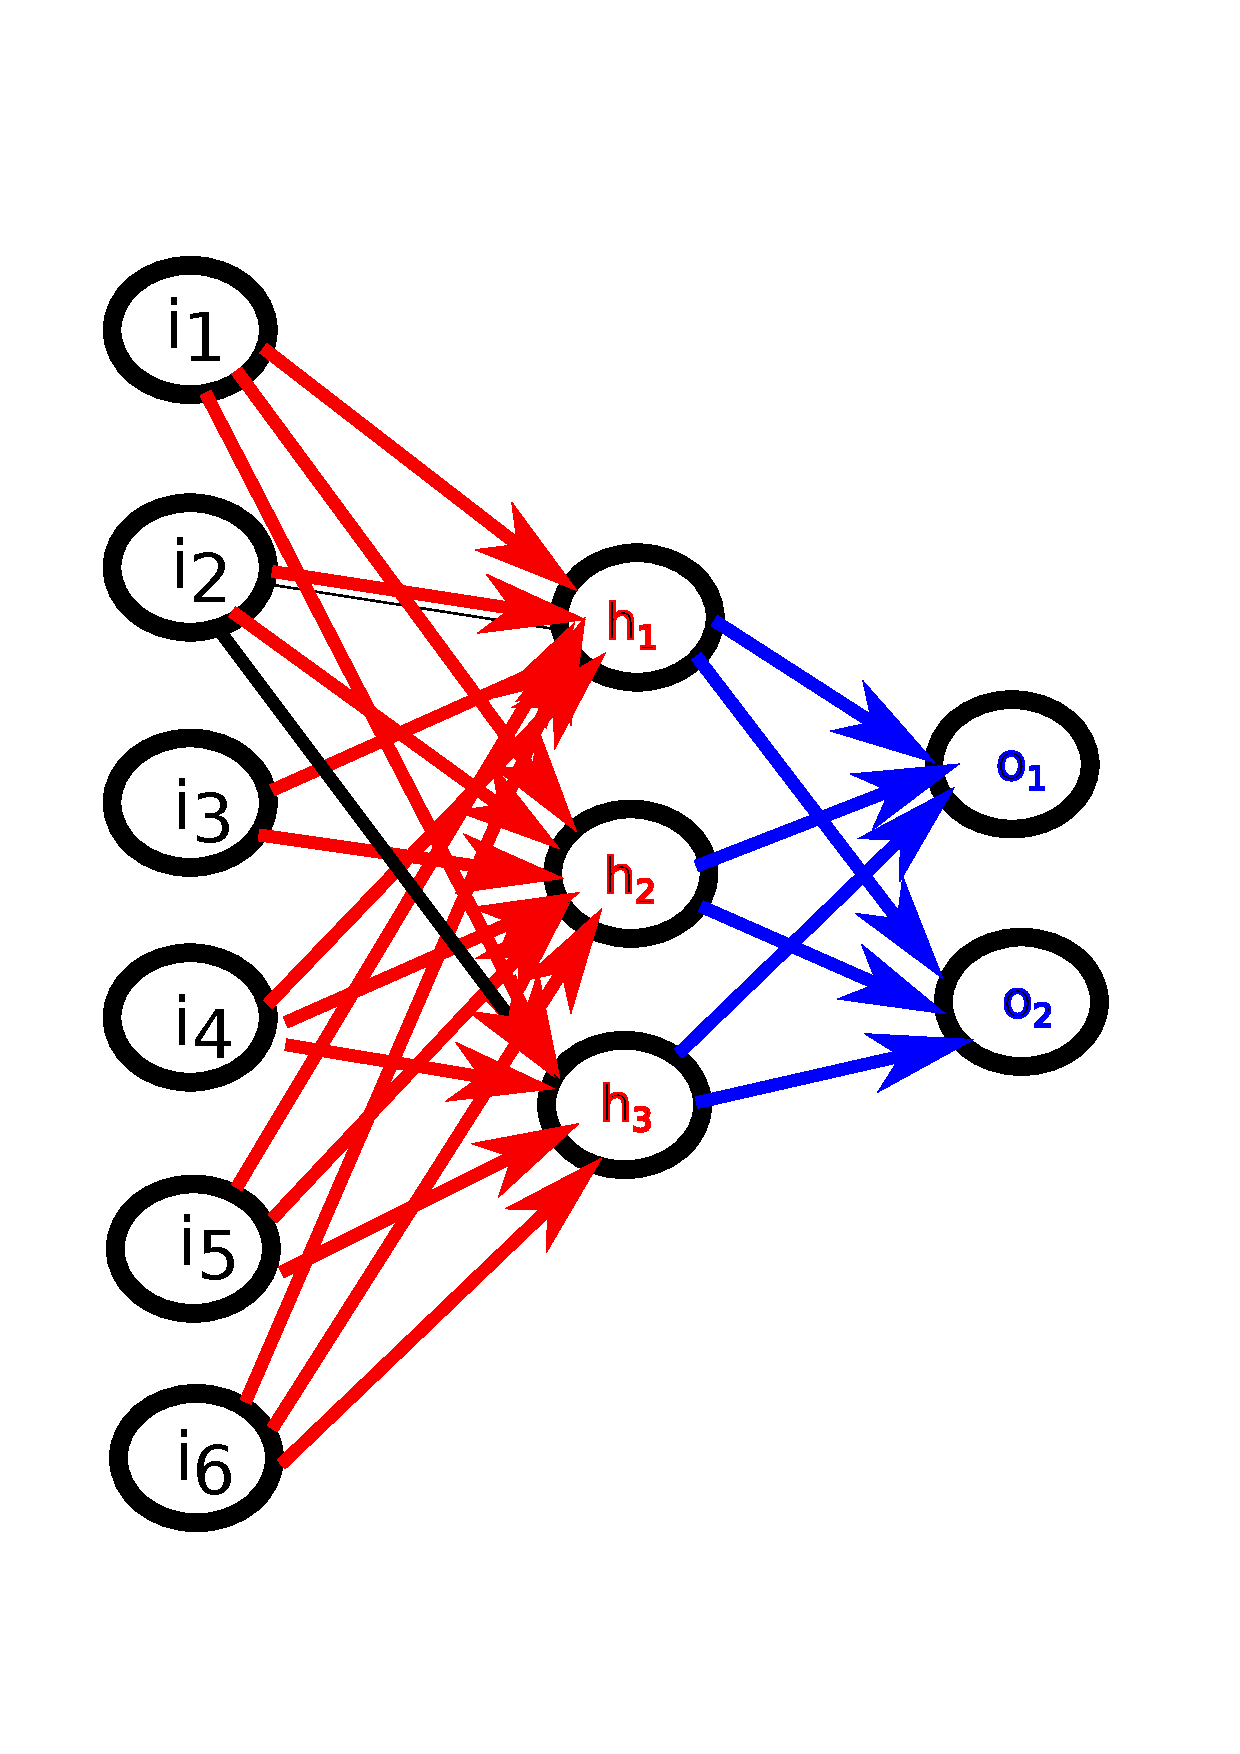
\includegraphics[width=0.7\textwidth]{full.pdf}
       \end{center}
      \caption{A fully connected network. The red connections can be organised
      in $3\times 6$ matrix $\boldsymbol{V}$, the blue connections in 1 $2 \times 3$ matrix $\boldsymbol{W}$.}
      \label{fig-connected}
    \end{figure}

    Mathematically, the relation between input and output can be described as follows:
    \begin{equation}
      \boldsymbol{o} = f( \boldsymbol{W} \boldsymbol{h} ) = f(\boldsymbol{W} g(\boldsymbol{V} \boldsymbol{i}))
    \end{equation}
    Here $\boldsymbol{i}$ is an array of $I$ nodes, the values which are set by the user. The is called \emph{entering an input pattern into the network.}
    There are $H$ hidden nodes, and $O$ output nodes. $\boldsymbol{V}$ is a $H \times I$ matrix, and $\boldsymbol{W}$ is a $O \times H$ matrix.
    The products $\boldsymbol{V} \boldsymbol{i}$ is matrix-vector multiplication, so is of the form: $ \sum^{H}_{q=1} V_{pq} i_q$, where
    $V_{pq}$ are the components of matrix $\boldsymbol{V}$ and $i_q$ is a component of vector $\boldsymbol{I}$. A squashing function $g(x)$ is applied node-wise
    to the output of the matrix vector multiplication, which defines the values of vector $\boldsymbol{H}$. A second calculation takes place that carries the
    values of the hidden layer into the output layer. This entails a matrix vector multiplication of the matrix $\boldsymbol{W}$ with the values of $\boldsymbol{H}$
    and the squashing function $f(x)$ is applied node-wise on the result of this calculation.

    Writing this explicitly in terms of the components makes clear that this is a relatively convoluted expression:
    \begin{equation}
      o_i = f( \sum_{j} w_{ij}g(\sum_k v_{jk} i_k)) = f(\sum_j w_{ij}h_j)
      \label{eq-update}
    \end{equation}


    Eq. \ref{eq-update} is a very fundamental equation. It describes how multi-layer perceptrons operate on an input pattern. Computationally the most expensive
    part of this are the matrix-vector multiplications as the matrices $\boldsymbol{v}, \boldsymbol{w}$ can be very large. Moreover, we have restricted ourselves
    for demonstration purposes to a three-layer network. There is no need for this restriction, and indeed networks can be much deeper, requiring dozens of matrices.
    One of the technical developments that have made neural networks viable as a computational technique is that matrix-vector multiplications can be highly parallelised.
    Each node in the output vector can be calculated independent of any other node. Since these operations are very typical in graphics operations, modern
    computers contain a graphics card with dedicated hardware called a GPU, which is designed to perform a large number of such operations in parallel. It was quickly
    realised that neural networks can parallelised in a similar way because within each layer computation of node values can be done in parallel. Nowadays, large
    networks are always trained on a GPU. Modern neural network software makes the use of GPUs completely transparent, as we will see.
    
    
    As before, we can define a loss function, which could be an MSE loss function, or cross entropy. We will use the MSE loss in the discussion below, but the same ideas
    apply to cross entropy or other loss functions.

    For MSE the loss function is defined as:
    \begin{equation}
      \mathcal{L} = \sum_i \frac{1}{2}(\boldsymbol{o}_i - \boldsymbol{d}_i)^2
      \label{eq-lossmse}
    \end{equation}
    We will discuss the backpropagation from a regression point of view, later returning to classification. We assume that for each data point $\boldsymbol{x}_i$, we have
    a desired regression value $\boldsymbol{d}_i$. Note that $\boldsymbol{x}$ and $\boldsymbol{d}$ are vectors, and that the summation in Eq. \ref{eq-lossmse} runs over
    \emph{data points}, whereas the summations in Eq. \ref{eq-update} run over nodes for a single given input vector $\boldsymbol{i}$.

    As in logistic regression, we want to calculate the gradient of the loss function with respect to the weights $\boldsymbol{v}, \boldsymbol{w}$, so that we can
    incorporate it in a stochastic gradient descent algorithm. This might seem like a major problem for the weights $\boldsymbol{v}$, which appear deeply embedded
    in two functions $f$ and $g$ that both could be non linear. The existence of a relatively simple algorithm to solve this problem was one of the conceptual
    breakthroughs that made neural networks possible.


    

    \section{The Backpropagation Algorithm}
    The algorithm that we will discuss in this section is called backpropagation by error. It refers to a method for calculating the gradient of the loss function
    with respect to the weights, and the reason for this name will become clear below. Its derivation is nothing more than a repeated application of the chain rule
    of calculus. You should review this, if you are not confident in its use, e.g.. here: \url{https://tutorial.math.lamar.edu/problems/calci/diffformulas.aspx}.

    The gradient with respect to the $\boldsymbol{w}$ matrix is similar to the procedure we followed for a  single neuron. The main difference here is that
    we can have more than one output neuron. Our vector of input weights now becomes a matrix, but apart from that nothing changes:

    \begin{equation}
      \frac{\partial \mathcal{L}}{\partial \boldsymbol{w}} = \sum_i (\boldsymbol{o}^{(i)} - \boldsymbol{d}^{(i)})\frac{\partial o^{(i)}}{\partial \boldsymbol{w}}
      \label{eq-grad}
    \end{equation}
    We derive the batch version of the algorithm where we calculate the gradient over all data points, we will discuss variations later. To distinguish between
    data points indices, which tells us which input output pair from the dataset we are dealing with, and node labels that tells us which node we are discussing,
    we use brackets in the data point indices.

    Next, we will use the fact that derivatives are linear. So we can calculate the gradient for every data point, do this for each data point and then add the result
    to obtain the gradient of the batch. Below, we will show the gradient calculation for a single data point, say point (1), but since the calculation is identical
    for all data points, we drop the label for notational convenience. Every index in the calculations below will label a node until further notice.

    For a single data point, our loss function is:
    $$
    \mathcal{L} = \frac{1}{2}\sum_k (o_k - d_k)^2,
    $$
    i.e. the sum of the node-wise difference squared divided by 2. The gradient with respect weight $w_{pq}$ is:
    \begin{equation}
      \frac{\partial \mathcal{L}}{\partial w_{pq}} = \sum_k (o_k - d_k)\frac{\partial o_k}{\partial w_{pq}}
      \label{eq-partdiff}
    \end{equation}
    
    Since,
    \begin{equation}
    \frac{\partial o_k}{\partial w_{pq}} = f^{\prime}(\sum_j w_{kl} h_l) \frac{\partial \sum_l w_{il}h_l}{\partial w_{pq}} = f^{\prime}(\sum_j w_{kl}h_l)\sum_l \delta^p_k \delta^q_l h_l
    \end{equation}

    The Kronecker delta is defined by:

    $$
    \delta^i_j = \left\{ \begin{array}{rl} i \ne j: & 0 \\ i = j: & 1 \end{array} \right.
    $$

    This is a convenient way of expressing that $\frac{\partial w_{pq}}{\partial w_{kl}}$ in general is zero, unless $p=i$ and $q=j$.
    The result can be written as:
    \begin{equation}
      \frac{\partial o_k}{\partial w_{pq}} = f^{\prime}(\sum_j w_{kj}h_j) \delta^p_i h_q 
    \end{equation}
    Substituting this back into Eq. \ref{eq-partdiff} gives:
    \begin{align}
     \frac{\partial \mathcal{L}}{\partial w_{pq}} &  = (o_p -d_p)f^{\prime}(\sum_l w_{kl} h_l) h_q  \nonumber \\
                                         & = \Delta^{\boldsymbol{W}}_p h_q,
     \end{align}
     
    This is essentially the graded perceptron learning rule that we derived earlier, plus a $\Delta$ symbol that expresses that the gradient of node $p$ does not depend
    on weights that lead to other nodes than node $p$ (remember: in general, there will be other nodes in the output layer, but their weights do not affect the gradient
    of this node).

    When $f^{\prime}$ is the logistic function, $f^{\prime}(\sum_j w_{kj}h_j) = o_k(1 - o_k)$, but we will no longer make the assumption that the logistic function is the
    only squashing function that is generally applied.  Once the squashing
    function has been decided the awkward looking $f^{\prime}$ terms always reduce to something simple. For now, we will leave them in.

    The derivative with respect to the matrix $\boldsymbol{V}$ is a repeated application of the chain rule.
    We now need to make the dependency explicit:
    $$
    o_k = f(\sum w_{kl} h_l) = f(\sum_l w_{kl}g(\sum_m v_{lm} l_m)).
    $$
    The since the $\boldsymbol{V}$ matrix is embedded inside two function calls, we need to apply the chain rule twice:
    $$
    \frac{\partial o_k}{\partial v_{pq}} = f^{\prime}(\sum_l w_{kl}h_l) \sum_r w_{kr}g^{\prime}(\sum_m v_{rm} i_m) \sum_s \frac{\partial}{\partial v_{pq}} v_{rs} i_s,
    $$
    which works out as:
    $$
    \frac{\partial o_k}{\partial v_{pq}} = f^{\prime}(\sum_l w_{kl} h_l) w_{kp} g^{\prime}(\sum_m v_{pm}i_m) i_q.
    $$
    This gives:
    \begin{align}
      \frac{\partial \mathcal{L}}{\partial w_{pq}} & = \sum_k (o_k - d_k) f^{\prime}( \sum w_{kl} h_l ) w_{kp} g^{\prime}( \sum_m v_{pm} i_m)  \nonumber \\
      & = \sum_k \Delta^{\boldsymbol{w}} w_{kp} g^{\prime}(\sum_m v_{pm} i_m) i_q \nonumber \\
      & =  \Delta^{\boldsymbol{W}}_p i_q,
      \label{eq-output}
    \end{align}

    Here, we introduced:
    \begin{equation}
      \Delta^{\boldsymbol{V}} = \sum_k \Delta^{\boldsymbol{W}}_k w_{kp} g^{\prime}( \sum_m v_{pm} i_m)
      \label{eq-backprop}
   \end{equation}

    Eq. \ref{eq-backprop} is our central result. Observe that the sum runs over the first index, contrary to most formulae we introduced so far. 

    You will not be assessed on replicating this formula, although it is useful that you try to follow the derivation.
    Without at least sketching the backpropagation algorithm, it would
    be hard to understand how modern machine learning frameworks help you to use it. We will discuss this in detail in Sec. \ref{sec-interpretation} and will
    give examples of its practical use in notebook \emph{Backpropagation in Action}. Before we do that, we will give a heuristic explanation for why a hidden layer provides much
    of the computational power of neural networks.
    
    \section{The Role of the Hidden Layer: A Heuristic Explanation}
    \begin{figure}[!ht]
      \begin{center}
        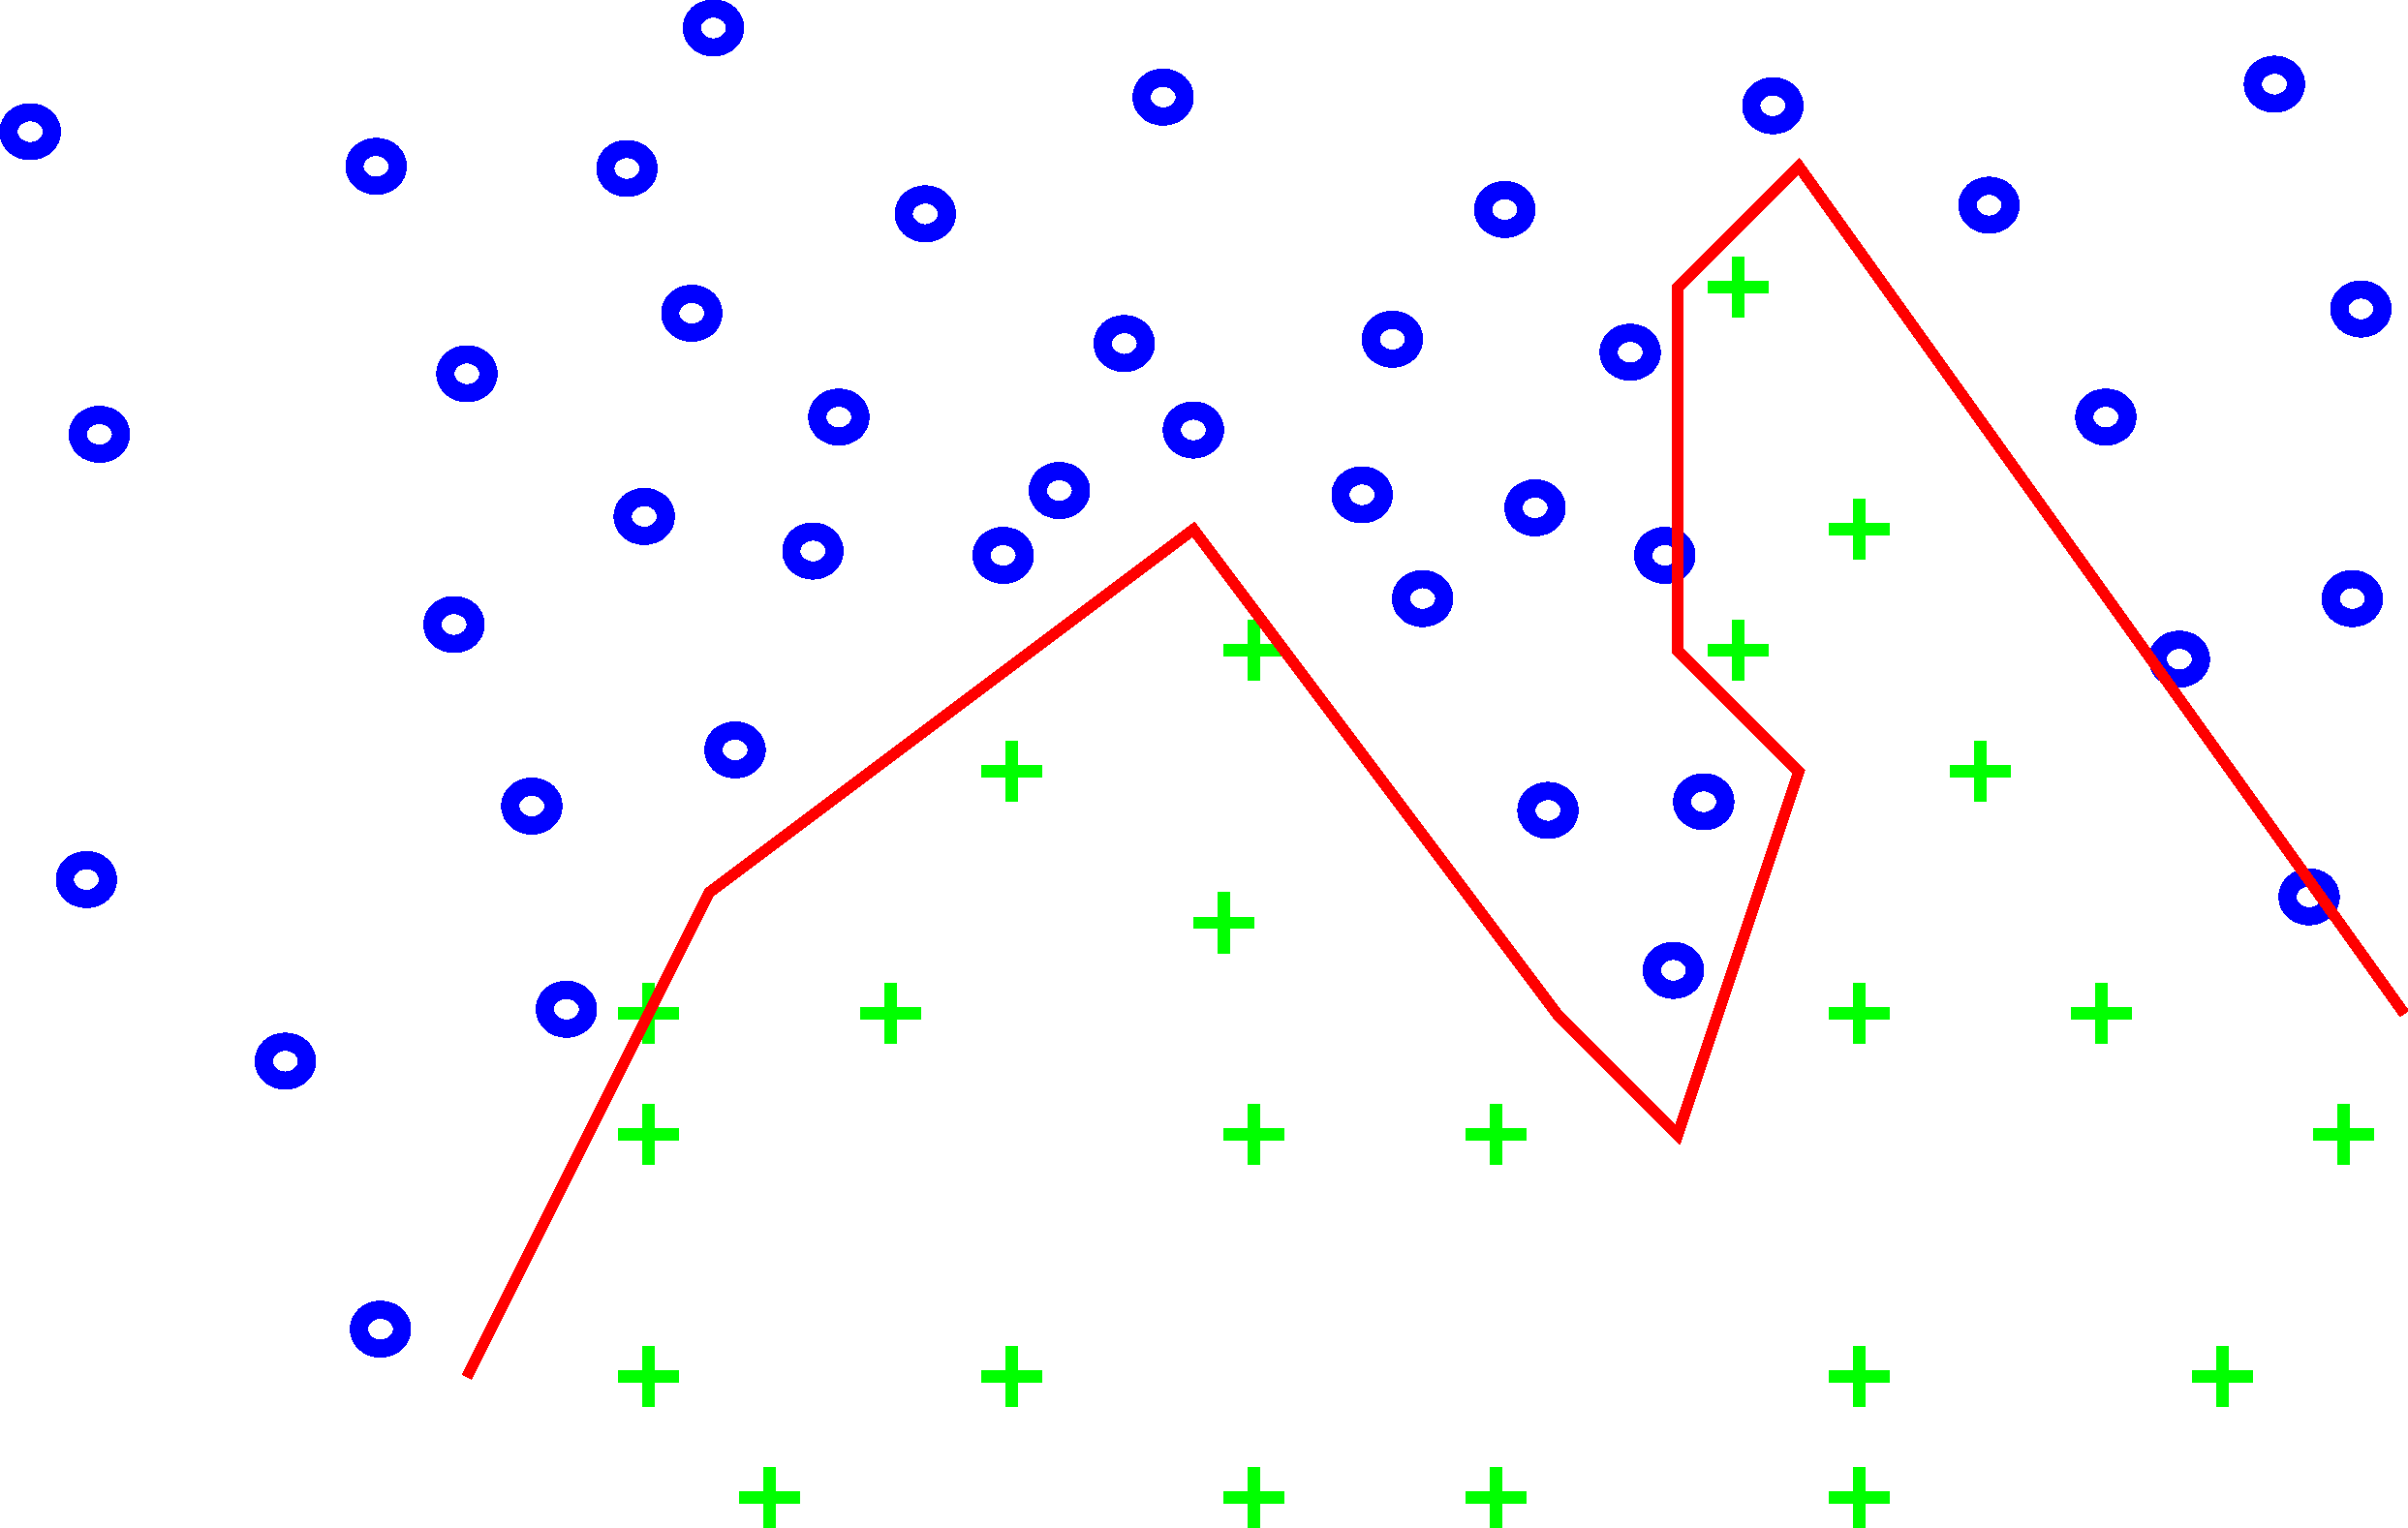
\includegraphics[width=0.7\textwidth]{decisionboundary.pdf}
      \end{center}
      \caption{A multilayer perceptron can be naively thought of as using higher layers to combine lower level decision boundaries, which are linear, into
        more complex non-linear ones.}
      \label{fig-boundary}
    \end{figure}

    One way of thinking about multilayer perceptrons is to consider the higher layers as organising decisions made on the basis of linear decision layers of individual
    perceptrons into more complex ones (Fig. \ref{fig-boundary}.
    Adding hidden noes therefore allows more combinations and therefore increases the computational power of the network. An example is given in \emph{Activity Multilayered Perceptron},
    where you will explore the increased possibilities of a multilayer neural network. The non-linearity of these hidden nodes is essential. Consider
    Eq. \ref{eq-update} when $g(x) = x$. It reads:
    $$
    o_i = f( \sum_{j} w_{ij}\sum_k v_{jk} i_k)),
    $$
    but $\sum_j w_{ij} v_{jk}$ is just another matrix $u_{ik}$, so:
    $$
    o_i = f(\sum_k u_{ik} i_k),
    $$
    but this describes just a two-layer network. If the hidden nodes are linear they just carry out a matrix-vector multiplication and we already have seen that a two-layer
    neural network is simply a group of perceptrons that has been switched in parallel with all the weaknesses of a single perceptron.

    What is true for classification networks is also true for regression networks.
    \begin{figure}[!ht]
      \begin{center}
        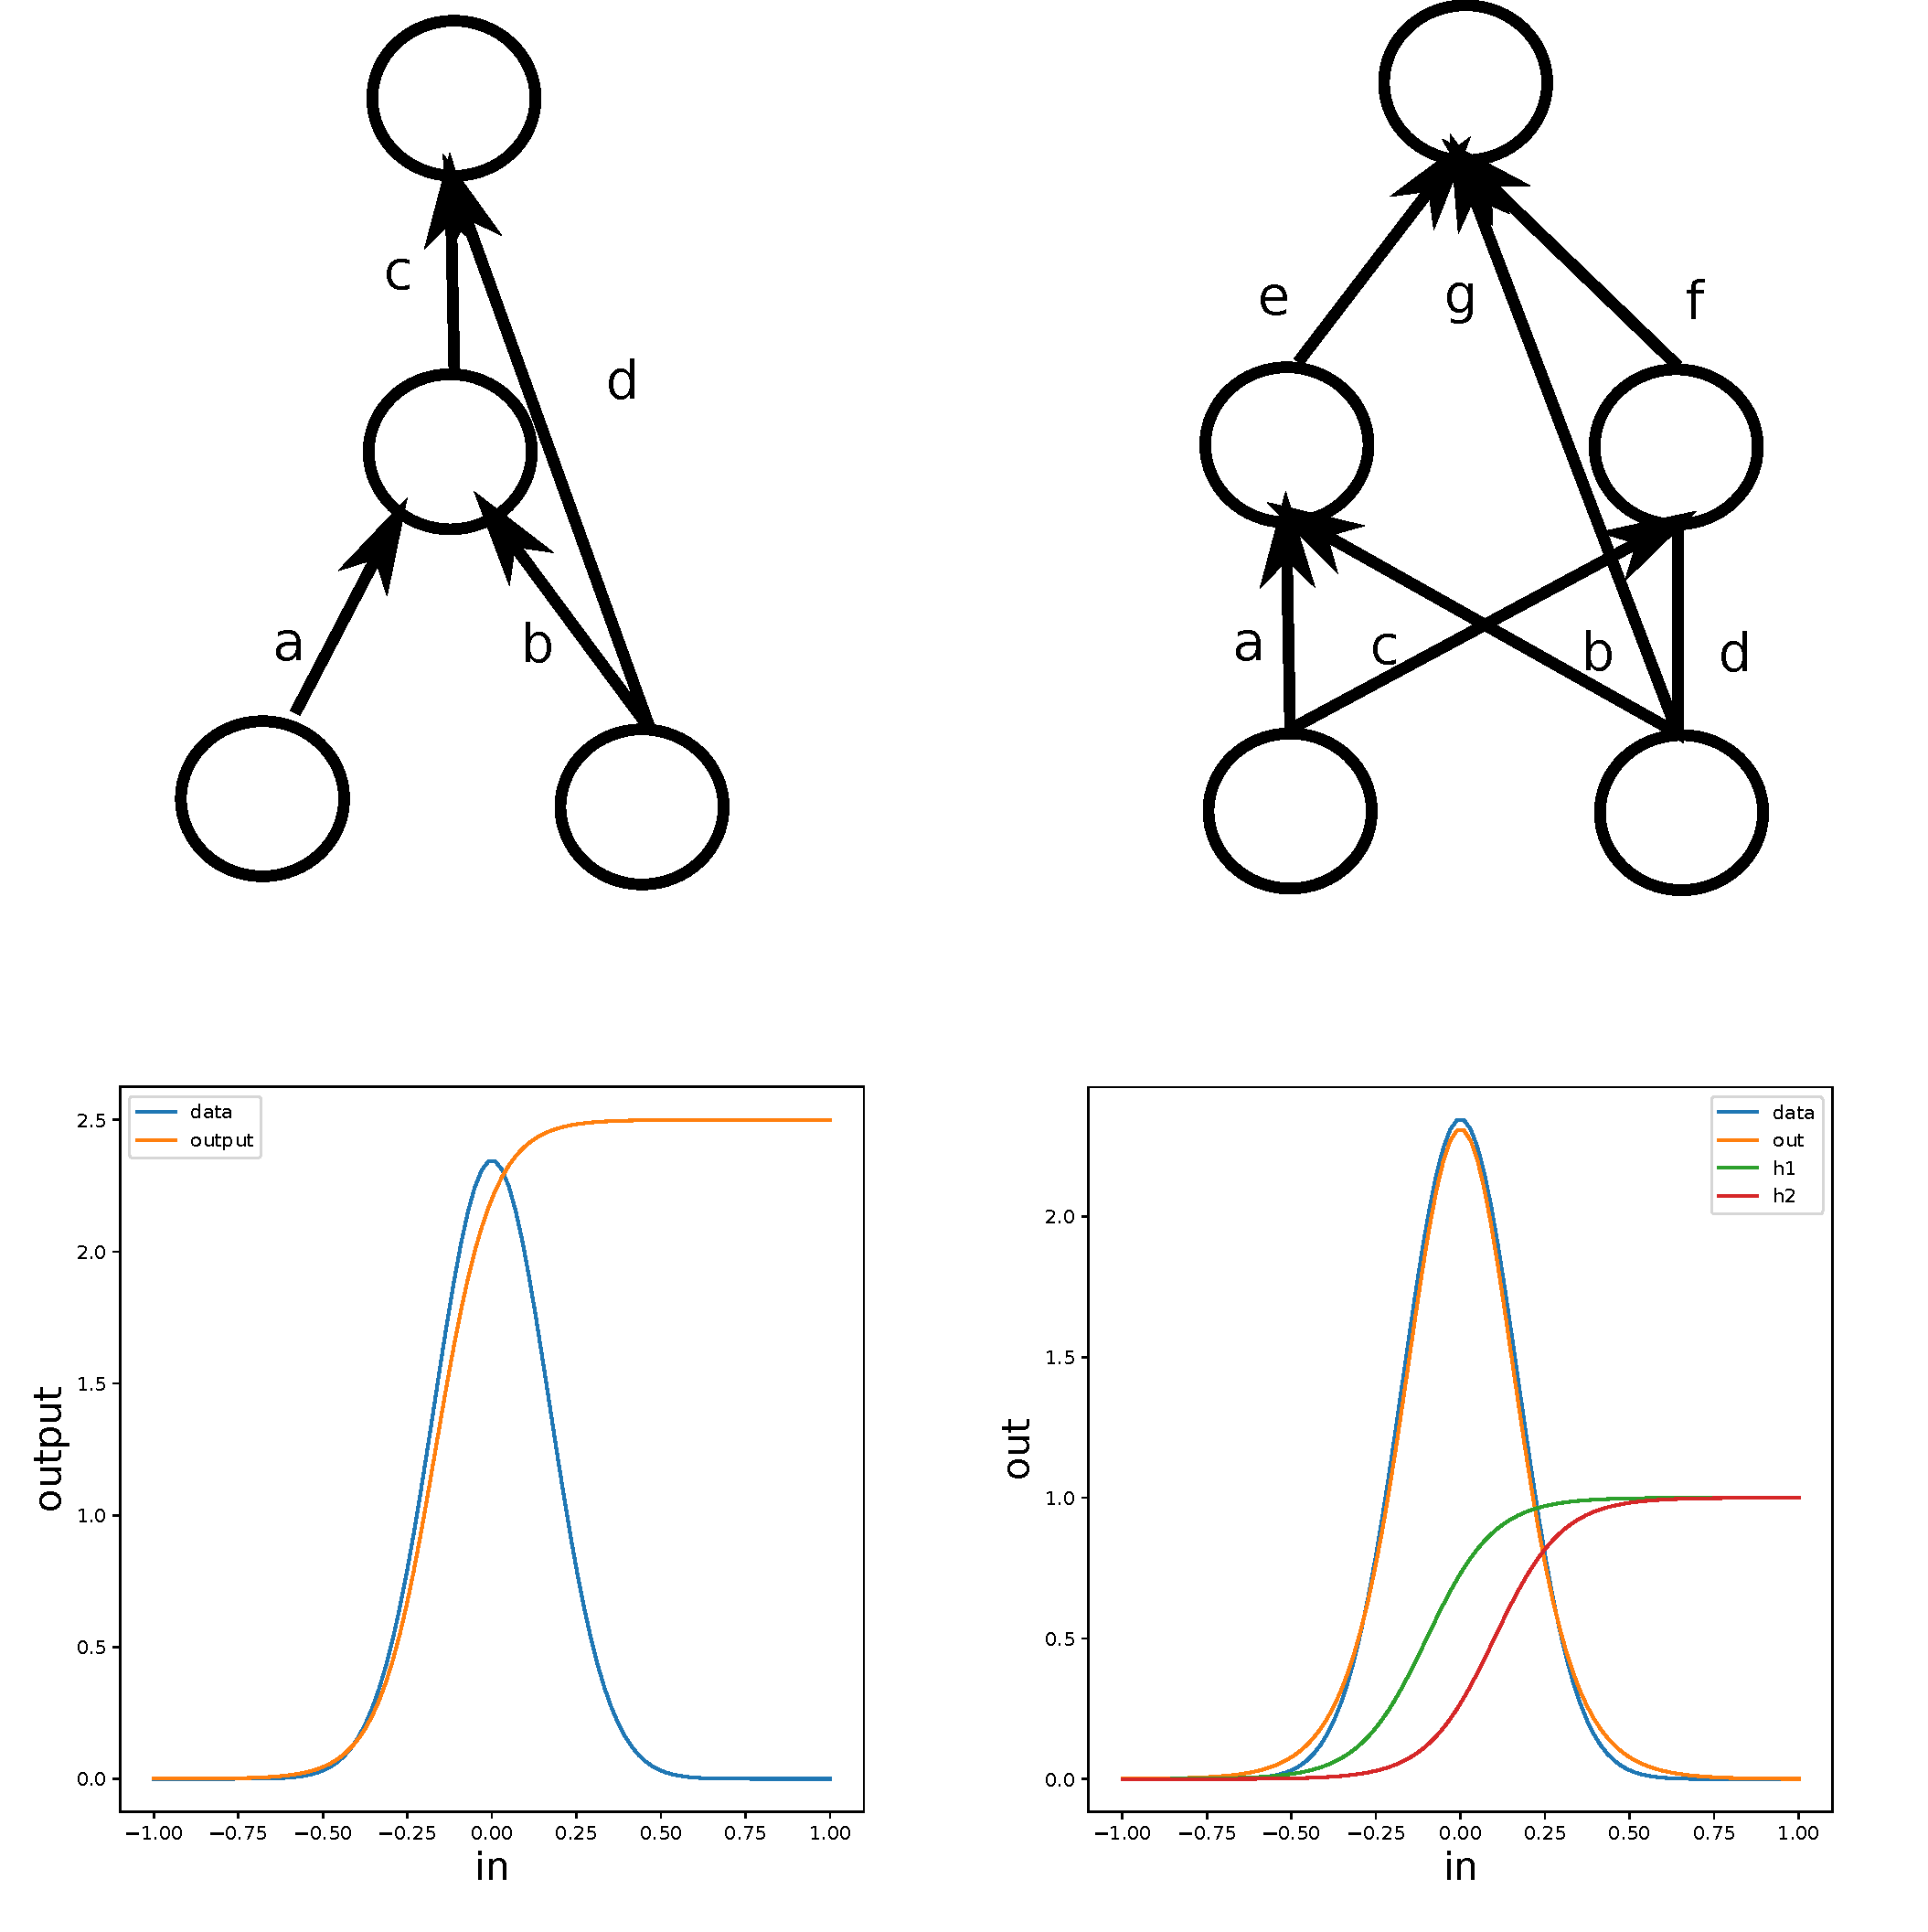
\includegraphics[width=0.7\textwidth]{hidden1.pdf}
      \end{center}
      \caption{Two of the simplest neural network architectures conceivable. The one with one node is only able to capture one trend in the data. At least two nodes
        are necessary to capture data with a peak. Observe that the two hidden nodes respond in a similar way, but their responses combined captures the data quite well.}
      \label{eq-arch}
    \end{figure}

    
    \section{Interpretation of the Backpropagation Algorithm}
    \label{sec-interpretation}
    Equation \ref{eq-update} has a clear network interpretation: information is entered in the input layer. The hidden layer is then evaluated, essentially
    by a matrix vector multiplication, and then the output layer, again by a matrix vector multiplication. This can easily be pictured as information
    flowing through the network.

    In a similar way, Eq. \ref{eq-backprop} can be interpreted as a measure of error that is transported back through the network. To see this, consider
    the quantity $\Delta^{\boldsymbol{w}}$ in Eq. \ref{eq-output}. It would be 0 if $d_k = o_k$, and is only non-zero when the desired output of the network and the actual
    output differ.

    Equation \ref{eq-backprop} can be interpreted as the error being entered in the output nodes, and propagated back to the hidden layer. To see this have a look at
    the fully connected network that we reproduce here, together with a reverse network.

    \begin{figure}[!ht]
      \begin{center}
        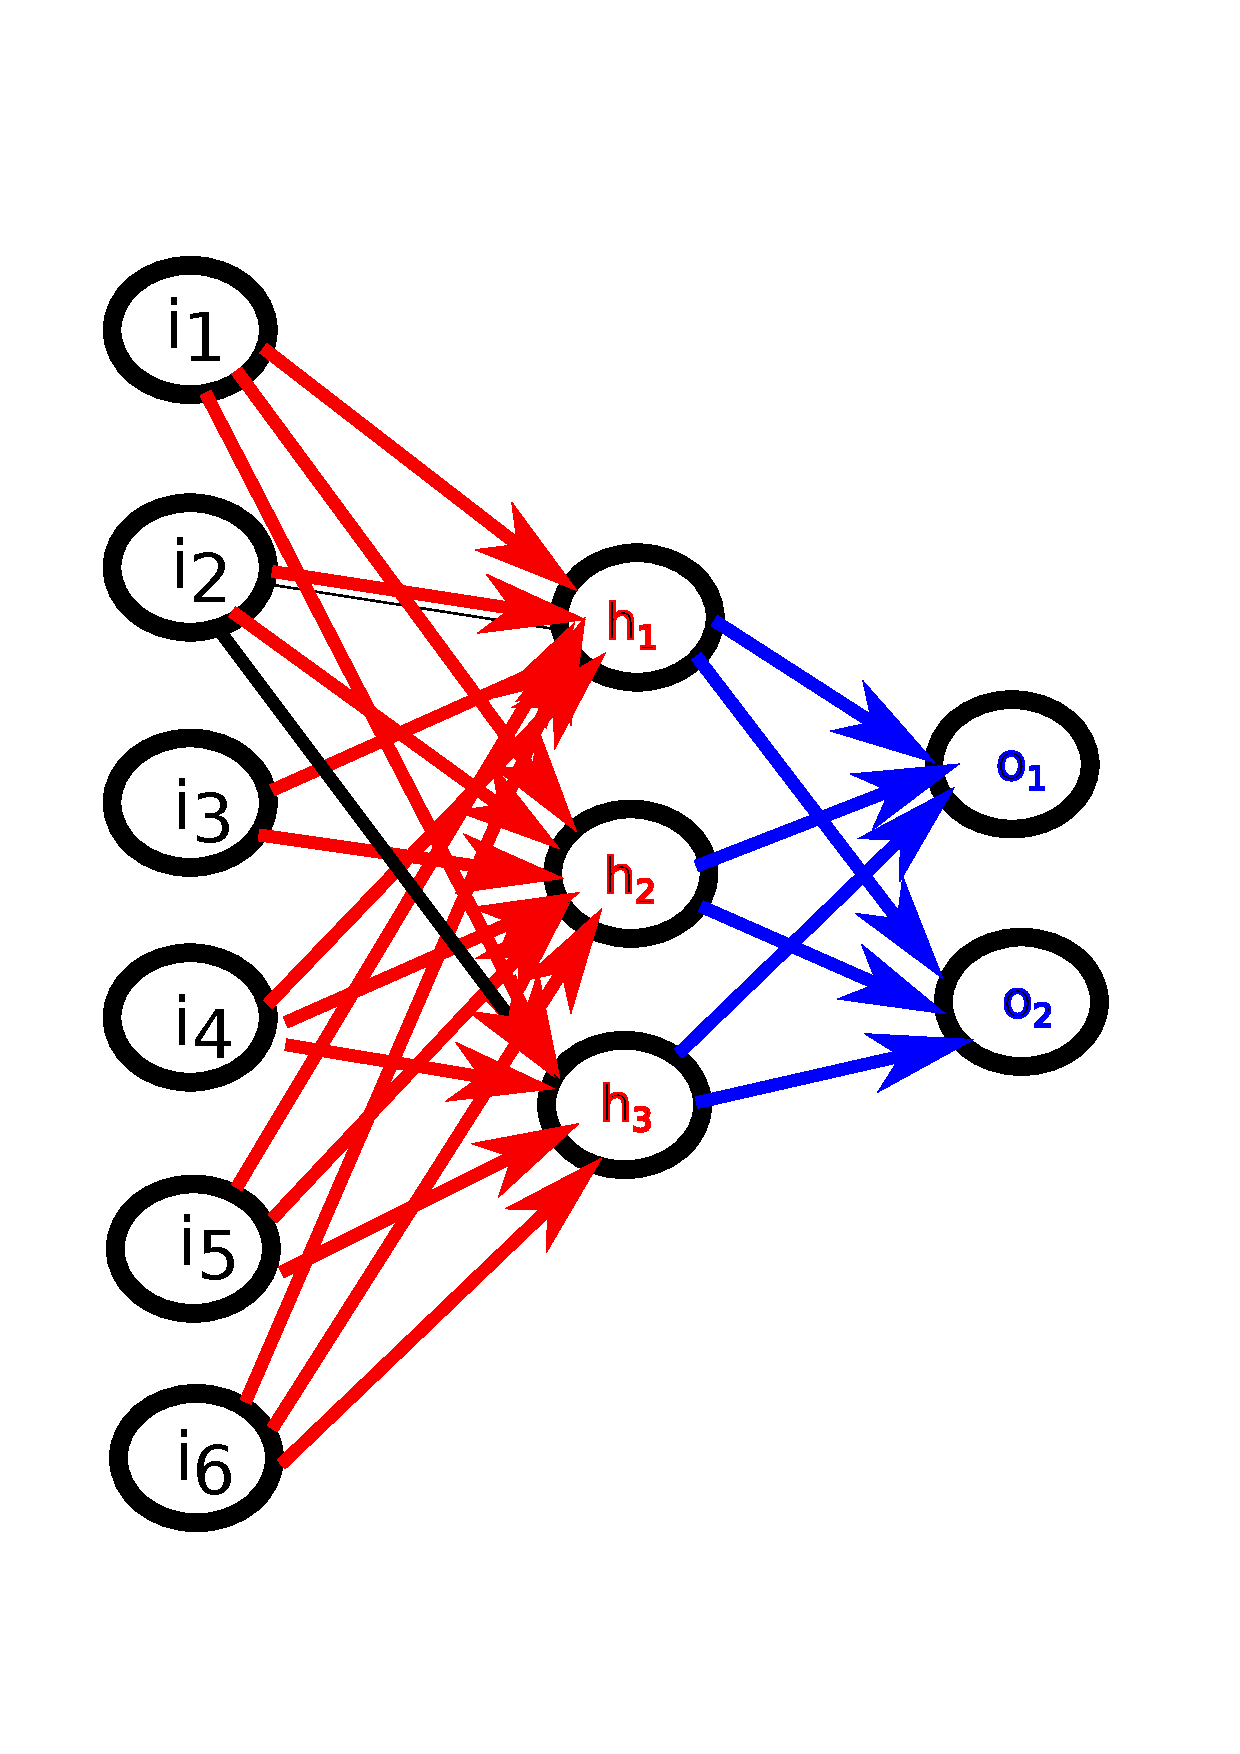
\includegraphics[width=0.7\textwidth]{full.pdf}
        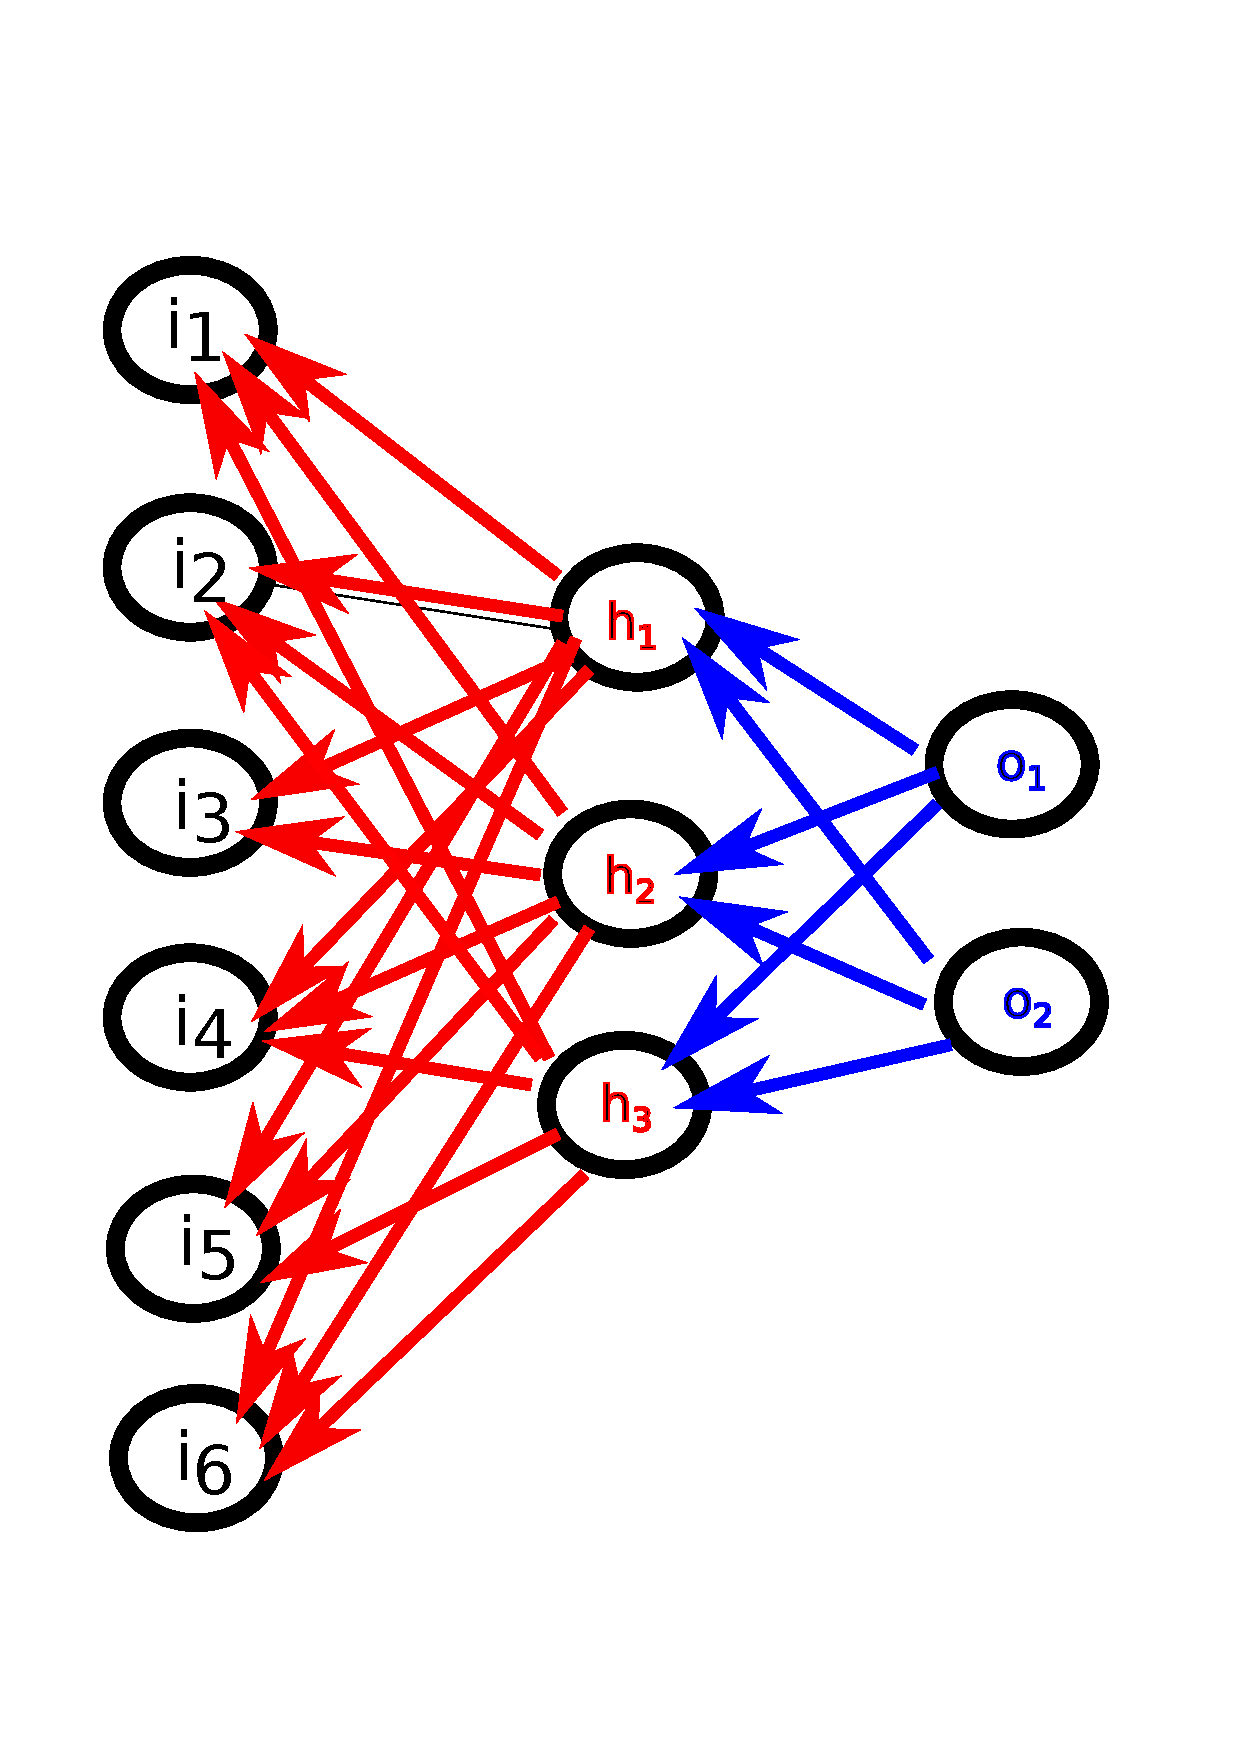
\includegraphics[width=0.7\textwidth]{fullreverse.pdf}
      \end{center}
      \caption{The update rule for the forward network is $o = f( \boldsymbol{W} g (\boldsymbol{V} \boldsymbol{i}))$. The update rule for the
        reverse network is $i = g(\boldsymbol{V}^T f(\boldsymbol{W}^T \boldsymbol{o}))$.}
    \end{figure}

    In a forward pass we first update the hidden layer by:
    $$
    h_i = \sum^6_{j=1}v_{ij}i_j,
    $$
    and then update the output layer:
    $$
    o_k = \sum^3_{l=1} w_{kl}h_l
    $$
    We use the convention here that in $v_{ij}$, the index $i$ labels the \emph{row} of the matrix, and $j$ the column.

    Now consider the reverse network, which has its input layer on the right. If we now where to update the hidden layer, we would
    calculate:
    $$
    h_i = \sum^2_{j=1} w_{ji}
    $$
    The summation here runs over the first index! Now consider Eq. \ref{eq-backprop}. It has exactly this form. At the output nodes we calculate
    $\Delta^{\boldsymbol{W}}$, which we feedback in the network. Then we do something at the nodes. Note that we only have to propagate $\Delta{\boldsymbol{W}}$
    back to the hidden layer. The gradient for the connection $v_{pq}$ is the product $i_p \Delta^{V}_q$.

    The name backpropagation is therefore warranted. Interestingly, the algorithm works similar for networks with more than one hidden layer: the error will
    be propagated back until the first hidden layer.

    As you can see, the backpropagation algorithm is relatively complex and needs to be adapted to the architecture of the network, the loss function and the
    squashing functions used in the network. The development of new neural networks always used to require  considerable amount of software development. Modern
    neural network frameworks such as \emph{TensorFlow}, \emph{Keras}, \emph{PyTorch} or \emph{Theano}, have a so-called \emph{autograd} facility. Networks
    can be created in terms of symbolic code, and learning algorithms can be automatically derived when loss function, architecture or other aspects of the network
    are changed. It is still important to understand the backpropagation algorithm, but it is no longer necessary to implement this yourself.
    In \emph{Activity: Autograd} you will experiment with the \emph{autograd} functionality of \emph{PyTorch} that can perform the calculation of gradients automatically.

    In \emph{Activity Multilayered Perceptron} you will be guided into building a neural network that can classify elements of the MNIST dataset using a multilayer perceptron.
  
  



  
